\documentclass[a4paper]{scrartcl}
\usepackage[utf8]{inputenc}
\usepackage{amssymb}
\usepackage{amsmath}
\usepackage{hyperref}
\usepackage{booktabs}
\usepackage{caption}
\usepackage{graphicx}
\usepackage{tikz}
\usepackage[toc,page]{appendix}
\graphicspath{{img/}}

\usepackage{listings}
\usepackage{color, colortbl}
\definecolor{codegreen}{rgb}{0,0.6,0}
\definecolor{codegray}{rgb}{0.5,0.5,0.5}
\definecolor{codeblack}{rgb}{0,0,0}
\definecolor{codepurple}{rgb}{0.58,0,0.82}
\definecolor{codeblue}{rgb}{0,0,0.6}
\definecolor{backcolour}{rgb}{0.95,0.95,0.95}
 
\lstdefinestyle{python}{
    backgroundcolor=\color{backcolour},   
    commentstyle=\color{codegreen},
    keywordstyle=\color{codeblue},
    numberstyle=\tiny\color{codegray},
    stringstyle=\color{codepurple},
    basicstyle=\footnotesize\ttfamily,
    breakatwhitespace=false,         
    breaklines=true,                 
    captionpos=t,
    keepspaces=true,                 
    language=Python,
    numbers=left,                    
    numbersep=5pt,                  
    showspaces=false,                
    showstringspaces=false,
    showtabs=false,                  
    tabsize=2
}

\lstdefinestyle{json}{
    backgroundcolor=\color{backcolour},   
    commentstyle=\color{codeblack},
    keywordstyle=\color{codeblack},
    numberstyle=\tiny\color{codeblack},
    stringstyle=\color{codeblack},
    basicstyle=\footnotesize\ttfamily,
    breakatwhitespace=false,         
    breaklines=true,                 
    captionpos=b,
    keepspaces=true,                 
    language=Python,
    numbers=none,                    
    showspaces=false,                
    showstringspaces=false,
    showtabs=false,                  
    tabsize=2
}
\usepackage{footnote}
\usepackage{refcount}

\usepackage{multicol}
\usepackage{multirow}
\usepackage{makecell}
\usepackage{array}
\newcolumntype{M}[1]{>{\centering\arraybackslash}m{#1}}
\def\zapcolorreset{\let\reset@color\relax\ignorespaces}
\def\colorrows#1{\noalign{\aftergroup\zapcolorreset#1}\ignorespaces}

%opening
\title{\LARGE BigchainDB: A Scalable Blockchain Database (DRAFT)}

\author{
  Trent McConaghy, 
  Rodolphe Marques,
  Andreas M\"{u}ller,\\
  Dimitri De Jonghe,
  Troy McConaghy,
  Greg McMullen,\\
  Ryan Henderson,
  Sylvain Bellemare,\\
  and
  Alberto Granzotto
}

\date{\normalsize June 8, 2016\\ascribe GmbH, Berlin, Germany}

\begin{document}

\maketitle

\begin{abstract}
This paper describes BigchainDB. BigchainDB fills a gap in the decentralization ecosystem: a decentralized
database, at scale. It points to performance of 1 million writes per second throughput, storing petabytes of data, and
sub-second latency. The BigchainDB design starts with a distributed database (DB), and through a set of
innovations adds blockchain characteristics: decentralized control, immutability, and creation \& movement
of digital assets. BigchainDB inherits characteristics of modern distributed databases: linear scaling in
throughput and capacity with the number of nodes, a full-featured NoSQL query language, efficient
querying, and permissioning. Being built on an existing distributed DB, it also inherits enterprise-hardened
code for most of its codebase. Scalable capacity means that legally binding contracts and certificates may
be stored directly on the blockchain database. The permissioning system enables configurations ranging
from private enterprise blockchain databases to open, public blockchain databases. BigchainDB is
complementary to decentralized processing platforms like Ethereum, and decentralized file systems like
InterPlanetary File System (IPFS). This paper describes technology perspectives that led to the BigchainDB
design: traditional blockchains, distributed databases, and a case study of the domain name system (DNS).
We introduce a concept called blockchain pipelining, which is key to scalability when adding blockchain-like
characteristics to the distributed DB. We present a thorough description of BigchainDB, an
analysis of latency, and preliminary experimental results. The paper concludes with a description of use cases.
\end{abstract}


\section{Introduction}\label{sec:intro}

\subsection{Towards a Decentralized Application Stack}

The introduction of Bitcoin \cite{nakamoto2009bitcoin} has triggered a new wave of decentralization in computing. 
Bitcoin illustrated a novel set of benefits: decentralized control, where ``no one'' owns or controls the network; immutability,
where written data is tamper-resistant (``forever''); and the ability to create \& transfer assets on the network, without reliance on a central entity.

The initial excitement surrounding Bitcoin stemmed from its use as a token of value, for example as an alternative to government-issued currencies.
As people learned more about the underlying blockchain technology, they extended the scope of the technology itself (e.g. smart contracts), as well as applications (e.g. intellectual property).

With this increase in scope, single monolithic ``blockchain'' technologies are being re-framed and refactored into building blocks at four levels of the stack:
\begin{enumerate}
 \item Applications
 \item Decentralized computing platforms (``blockchain platforms'')
 \item Decentralized processing (``smart contracts'') and decentralized storage (file systems, databases), and decentralized communication
 \item Cryptographic primitives, consensus protocols, and other algorithms
\end{enumerate}

\subsection{Blockchains and Databases}
We can frame a traditional blockchain as a database (DB), in the sense that it provides a storage mechanism.
If we measure the Bitcoin blockchain by traditional DB criteria, it’s terrible: throughput is just a few transactions per second (tps), latency before a single confirmed write is 10 minutes, and capacity is a few dozen GB.
Furthermore, adding nodes causes more problems: with a doubling of nodes, network traffic quadruples with no improvement in throughput, latency, or capacity.
It also has essentially no querying abilities: a NoQL\footnote{We are introducing the term NoQL to describe a database with essentially no query abilities. This term is not to be confused with the database company noql (\url{http://www.noql.com}).} database.

In contrast, a modern distributed DB can have throughput exceeding 1 million tps, capacity of Petabytes and beyond, latency of a fraction of a second, and throughput and capacity that increases as nodes get added.
Modern DBs also have rich abilities for insertion, queries, and access control in SQL or NoSQL flavors; in fact SQL is an international ANSI and ISO standard.

\subsection{The Need for Scale}
Decentralized technologies hold great promise to rewire modern financial systems, supply chains, creative industries, and even the Internet itself.
But these ambitious goals need scale: the storage technology needs throughput of up to millions of transactions per second (or higher), sub-second latency\footnote{It takes light 140 ms to make one trip around the world, or 70 ms halfway around. Some financial applications need 30-100 ms latency, though due to speed-of-light constraints those necessarily need to be more locally constrained. Section \ref{sec:latency} explores this in detail.}, and capacity of petabytes or more.
These needs exceed the performance of the Bitcoin blockchain by many orders of magnitude.

\subsection{BigchainDB : Blockchains Meet Big Data}
This paper introduces BigchainDB, which is for database-style decentralized storage: a blockchain database.
BigchainDB combines the key benefits of distributed DBs and traditional blockchains, with an emphasis on scale, as Table \ref{tab:bigchain_comparison} summarizes.

\begin{table}[h]
  \caption{BigchainDB compared to traditional blockchains, and traditional distributed DBs}
  \footnotesize
  \makebox[\textwidth][c]{
  \centering
  \setlength\extrarowheight{3pt}
  \begin{tabular}{ | m{\dimexpr 0.25\linewidth-2\tabcolsep} |
	  M{\dimexpr 0.25\linewidth-2\tabcolsep} |
	  M{\dimexpr 0.25\linewidth-2\tabcolsep} |
	  M{\dimexpr 0.25\linewidth-2\tabcolsep} |} \Xhline{4\arrayrulewidth}\rowcolor{black}
  				                  & \color{white} Traditional Blockchain & \color{white} Traditional Distributed DB & \color{white} BigchainDB \\\Xhline{4\arrayrulewidth}
  High Throughput; increases with nodes$\uparrow$ & - 		           & \checkmark                  & \checkmark          \\\hline
  Low Latency                                     & - 		           & \checkmark                  & \checkmark          \\\hline
  High Capacity; increases with nodes$\uparrow$   & - 		           & \checkmark                  & \checkmark          \\\hline
  Rich querying                                   & - 		           & \checkmark                  & \checkmark          \\\hline
  Rich permissioning                              & - 		           & \checkmark                  & \checkmark          \\\hline
  Decentralized control                           & \checkmark 		   & -                          & \checkmark          \\\hline
  Immutability                                    & \checkmark 		   & -                          & \checkmark          \\\hline
  Creation \& movement of digital assets          & \checkmark 		   & -                          & \checkmark          \\\hline
  Event chain structure				  & Merkle Tree            & - 				& Hash Chain          \\
  \Xhline{4\arrayrulewidth}
  \end{tabular}
  }
  \label{tab:bigchain_comparison}
\end{table}

We built BigchainDB on top of an enterprise-grade distributed DB, from which
BigchainDB inherits high throughput, high capacity, low latency, a full-featured efficient NoSQL query language, and permissioning.
Nodes can be added to increase throughput and capacity.

\begin{figure}[!ht]
  \centering
  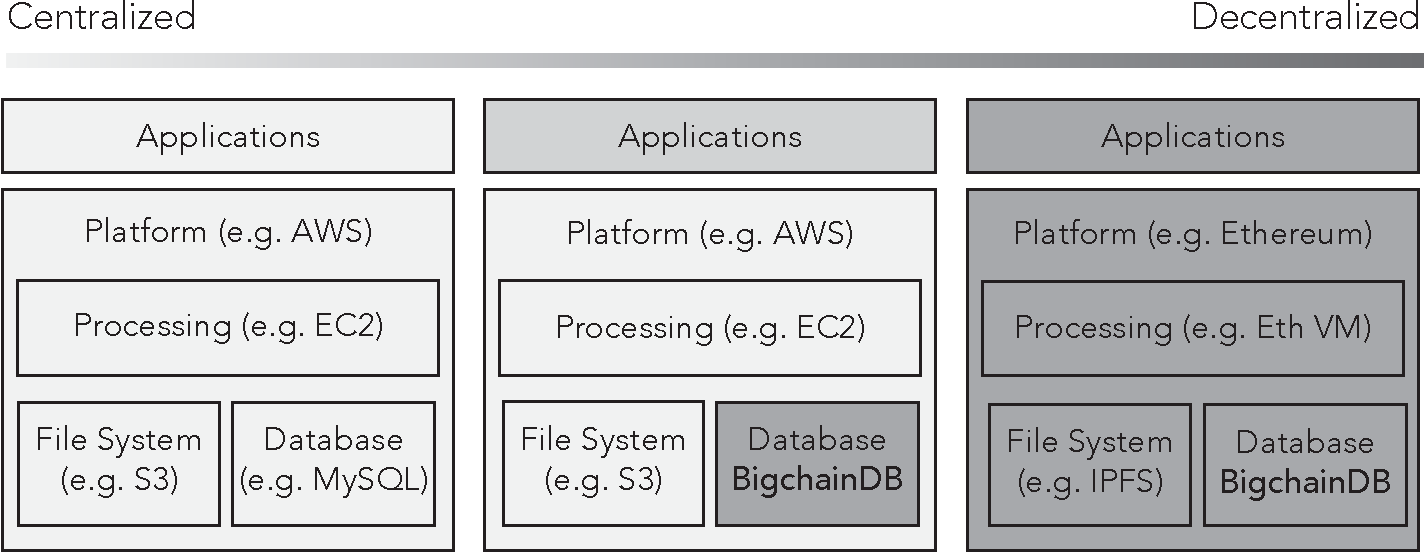
\includegraphics[width=\textwidth]{figure_1.pdf}
  \caption{From a base context of a centralized cloud computing ecosystem (left), BigchainDB can be added as another database to gain some decentralization benefits (middle).
  It also fits into a full-blown decentralization ecosystem (right).}
  \label{fig:bigchain_ecosystem}
\end{figure}

BigchainDB has the traditional blockchain benefits of decentralized control, immutability, and creation \& transfer of assets.
The decentralized control is via a federation of nodes with voting permissions, that is, a super-peer P2P network \cite{ozsu2011principles}.
The voting operates at a layer above the DB’s built in consensus.
Immutability / tamper-resistance is via an ordered sequence of blocks where each block holds an ordered sequence of transactions; and a block’s hash is over its transactions and related data, and the previous block’s hash; that is, a block chain.
Any entity with asset-issuance permissions can issue an asset; any entity with asset-transfer permissions and the asset’s private key may transfer the asset.
This means hackers or compromised system admins cannot arbitrarily change data, and there is no single-point-of-failure risk.

Scalable capacity means that legally binding contracts and certificates may be stored directly on the blockchain DB.
The permissioning system enables configurations ranging from private enterprise blockchain DBs to open, public blockchain DBs.
As we deploy BigchainDB, we are also deploying a public version.

\subsection{BigchainDB in the Decentralization Ecosystem}
Figure \ref{fig:bigchain_ecosystem} illustrates how BigchainDB can be used in a fully decentralized setting, or as a mild extension from a traditional centralized computing context.

BigchainDB is complementary to decentralized processing / smart contracts (e.g. Ethereum VM \cite{ethereum}\cite{buterin-ethereum} or Enigma \cite{enigma}\cite{zyskind2015enigma}), decentralized file systems (e.g. IPFS \cite{ipfs}), and communication building blocks (e.g. email).
It can be included in higher-level decentralized computing platforms (e.g. Eris/Tendermint \cite{eris}\cite{tendermint}).
It can be used side-by-side with identity protocols, financial asset protocols (e.g. Bitcoin \cite{nakamoto2009bitcoin}), intellectual property asset protocols (e.g. SPOOL \cite{dejonghe_spool}), and glue protocols (e.g. pegged sidechains \cite{back2010sidechains}, Interledger \cite{thomas2015interledger}).
Scalability improvements to smart contracts blockchains will help fully decentralized applications to better exploit the scalability properties of BigchainDB.

BigchainDB works with more centralized computing systems as well.
One use case is where decentralizing just storage brings the majority of benefit.
Another use case is where scalability needs are greater than the capabilities of existing decentralized processing technologies; in this case BigchainDB provides a bridge to an eventual fully-decentralized system.

\subsection{Contents}

This paper first gives background on related building blocks, with an eye to scale:
\begin{itemize}
 \item Section \ref{sec:background} - traditional blockchain scalability,
 \item Section \ref{sec:distributed} - distributed DBs, and
\end{itemize}


Then, this paper describes BigchainDB as follows:
\begin{itemize}
 \item Section \ref{sec:bigchaindb} - BigchainDB description,
 \item Section \ref{sec:implementation} - BigchainDB implementation, including capacity vs. nodes (Figure \ref{fig:bigchain_capacity_vs_nodes}),
 \item Section \ref{sec:latency} - BigchainDB latency analysis,
 \item Section \ref{sec:permissioning} - private vs. public BigchainDBs in a permissioning context,
 \item Section \ref{sec:benchmarks} - BigchainDB benchmarks, including throughput vs. nodes (Figure \ref{fig:bigchain_throughput_vs_nodes}),
 \item Section \ref{sec:deployment} - BigchainDB deployment, including use cases and timeline, and
 \item Section \ref{sec:conclusion} - conclusion.
\end{itemize}


The appendices contain:
\begin{itemize}
 \item Appendix \ref{appendix:glossary} - a glossary, e.g. clarifying “distributed” vs. “decentralized”,
 \item Appendix \ref{appendix:blockchain_scalability} - blockchain scalability proposals, and
 \item Appendix \ref{sec:dns} - the Domain Name System (DNS).
 \item Appendix \ref{appendix:benchmarks} – further BigchainDB benchmarks.
\end{itemize}
\section{Background: Traditional Blockchain Scalability}\label{sec:background}

This section discusses how traditional blockchains perform with respect to scalability, with an emphasis on Bitcoin.

\subsection{Technical Problem Description}
Technically speaking, a traditional blockchain is a distributed database (DB) that solves the “Strong Byzantine Generals” (SBG) problem \cite{koshy2014revolution}, the name given to a combination of the Byzantine Generals problem and the Sybil Attack problem.
In the Byzantine Generals problem \cite{lamport1982byzantine}, nodes need to agree on some value for a DB entry, under the constraint that the nodes may fail in arbitrary (malicious) ways.
The Sybil Attack problem \cite{douceur2002sybil} arises when one or more nodes figure out how to get unfairly disproportionate influence in the process of agreeing on a value for an entry.
It’s an “attack of the clones”—an army of seemingly independent voters actually working together to game the system.

\subsection{Bitcoin Scalability Issues}
Bitcoin has scalability issues in terms of throughput, latency, capacity, and network bandwidth.

\medskip
\noindent\textbf{Throughput.} The Bitcoin network processes just $1$ transaction per second (tps) on average, with a theoretical maximum of $7$ tps \cite{bitcoin2015scalability}.
It could handle higher throughput if each block was bigger, though right now making blocks bigger would lead to size issues (see Capacity and network bandwidth, below).
This throughput is unacceptably low when compared to the number of transactions processed by Visa ($2,000$ tps typical, $10,000$ tps peak) \cite{trillo2013visa}, Twitter ($5,000$ tps typical, $15,000$ tps peak), advertising networks ($500,000$ tps typical), trading networks, or email networks (global email volume is $183$ billion emails/day or $2,100,000$ tps \cite{sourabh2014email}).
An ideal global blockchain, or set of blockchains, would support all of these multiple high-throughput uses.

\medskip
\noindent\textbf{Latency.} Each block on the Bitcoin blockchain takes $10$ minutes to process.
For sufficient security, it is better to wait for about an hour, giving more nodes time to confirm the transaction.
By comparison, a transaction on the Visa network is approved in seconds at most.
Many financial applications need latency of $30$ to $100$~ms.

\medskip
\noindent\textbf{Capacity and network bandwidth.} The Bitcoin blockchain is about $70$~GB (at the time of writing); it grew by $24$~GB in $2015$ \cite{blockchaininfo2015blockchain_size}.
It already takes nearly a day to download the entire blockchain.
If throughput increased by a factor of $2,000$, to Visa levels, the additional transactions would result in database growth of $3.9$~GB/day or $1.42$~PB/year.
At $150,000$~tps, the blockchain would grow by $214$~PB/year (yes, petabytes).
If throughput were 1M tps, it would completely overwhelm the bandwidth of any node’s connection.

\subsection{Technology Choices Affecting Scalability}
The Bitcoin blockchain has taken some technology choices which hurt scaling:
\begin{enumerate}
 \item \textbf{Consensus Algorithm: POW.} Bitcoin’s mining reward actually incentivizes nodes to increase computational resource usage, without any additional improvements in throughput, latency, or capacity. A single confirmation from a node takes $10$ minutes on average, so six confirmations take about an hour. In Bitcoin this is by design; Litecoin and other altcoins reduce the latency, but compromise security.
 \item \textbf{Replication: Full.} That is, each node stores a copy of all the data; a “full node.” This copy is typically kept on a single hard drive (or in memory). Ironically, this causes centralization: as amount of data grows, only those with the resources to hold all the data will be able to participate.
\end{enumerate}

These characteristics prevent the Bitcoin blockchain from scaling up.

\subsection{Blockchain Scalability Efforts}
The Bitcoin / blockchain community has spent considerable effort on improving the performance of blockchains.
Appendix~\ref{appendix:blockchain_scalability} reviews various proposals in more detail.

Previous approaches shared something in common: they are all started with a block chain design then tried to increase its performance.
There’s another way: start with a ``big~data'' distributed database, then give it blockchain-like characteristics.
\section{Background: Distributed Databases \& Big Data}\label{sec:distributed}

\subsection{Introduction}
We ask: does the world have any precedents for \textit{distributed databases} at massive scale? The answer is yes.
All large Internet companies, and many small ones, run “big data” distributed databases (DBs), including Facebook, Google, Amazon and Netflix.
For example, at any given time Netflix might be serving up content making up $35\%$ of the bandwidth of the entire Internet \cite{spangler2014netflix}.

Distributed DBs regularly store petabytes ($1,000,000$ GB) or more worth of content. 
In contrast, the Bitcoin blockchain currently stores $50$ GB, the capacity of a modern thumb drive.
There are initiatives to prevent “blockchain bloat” caused by “dust” or “junk” transactions that “pollute” Bitcoin’s $50$ GB database \cite{wagner2014blockchain_bloat}.

In light of petabyte-capacity DBs, it is ironic that a $50$ GB database would be concerned by “bloat”.
But let’s look at it another way: perhaps distributed DB technology has lessons for blockchain DB design.

\medskip
\centerline{Let’s explore distributed DB scalability further.}

\begin{figure}[!ht]
  \centering
  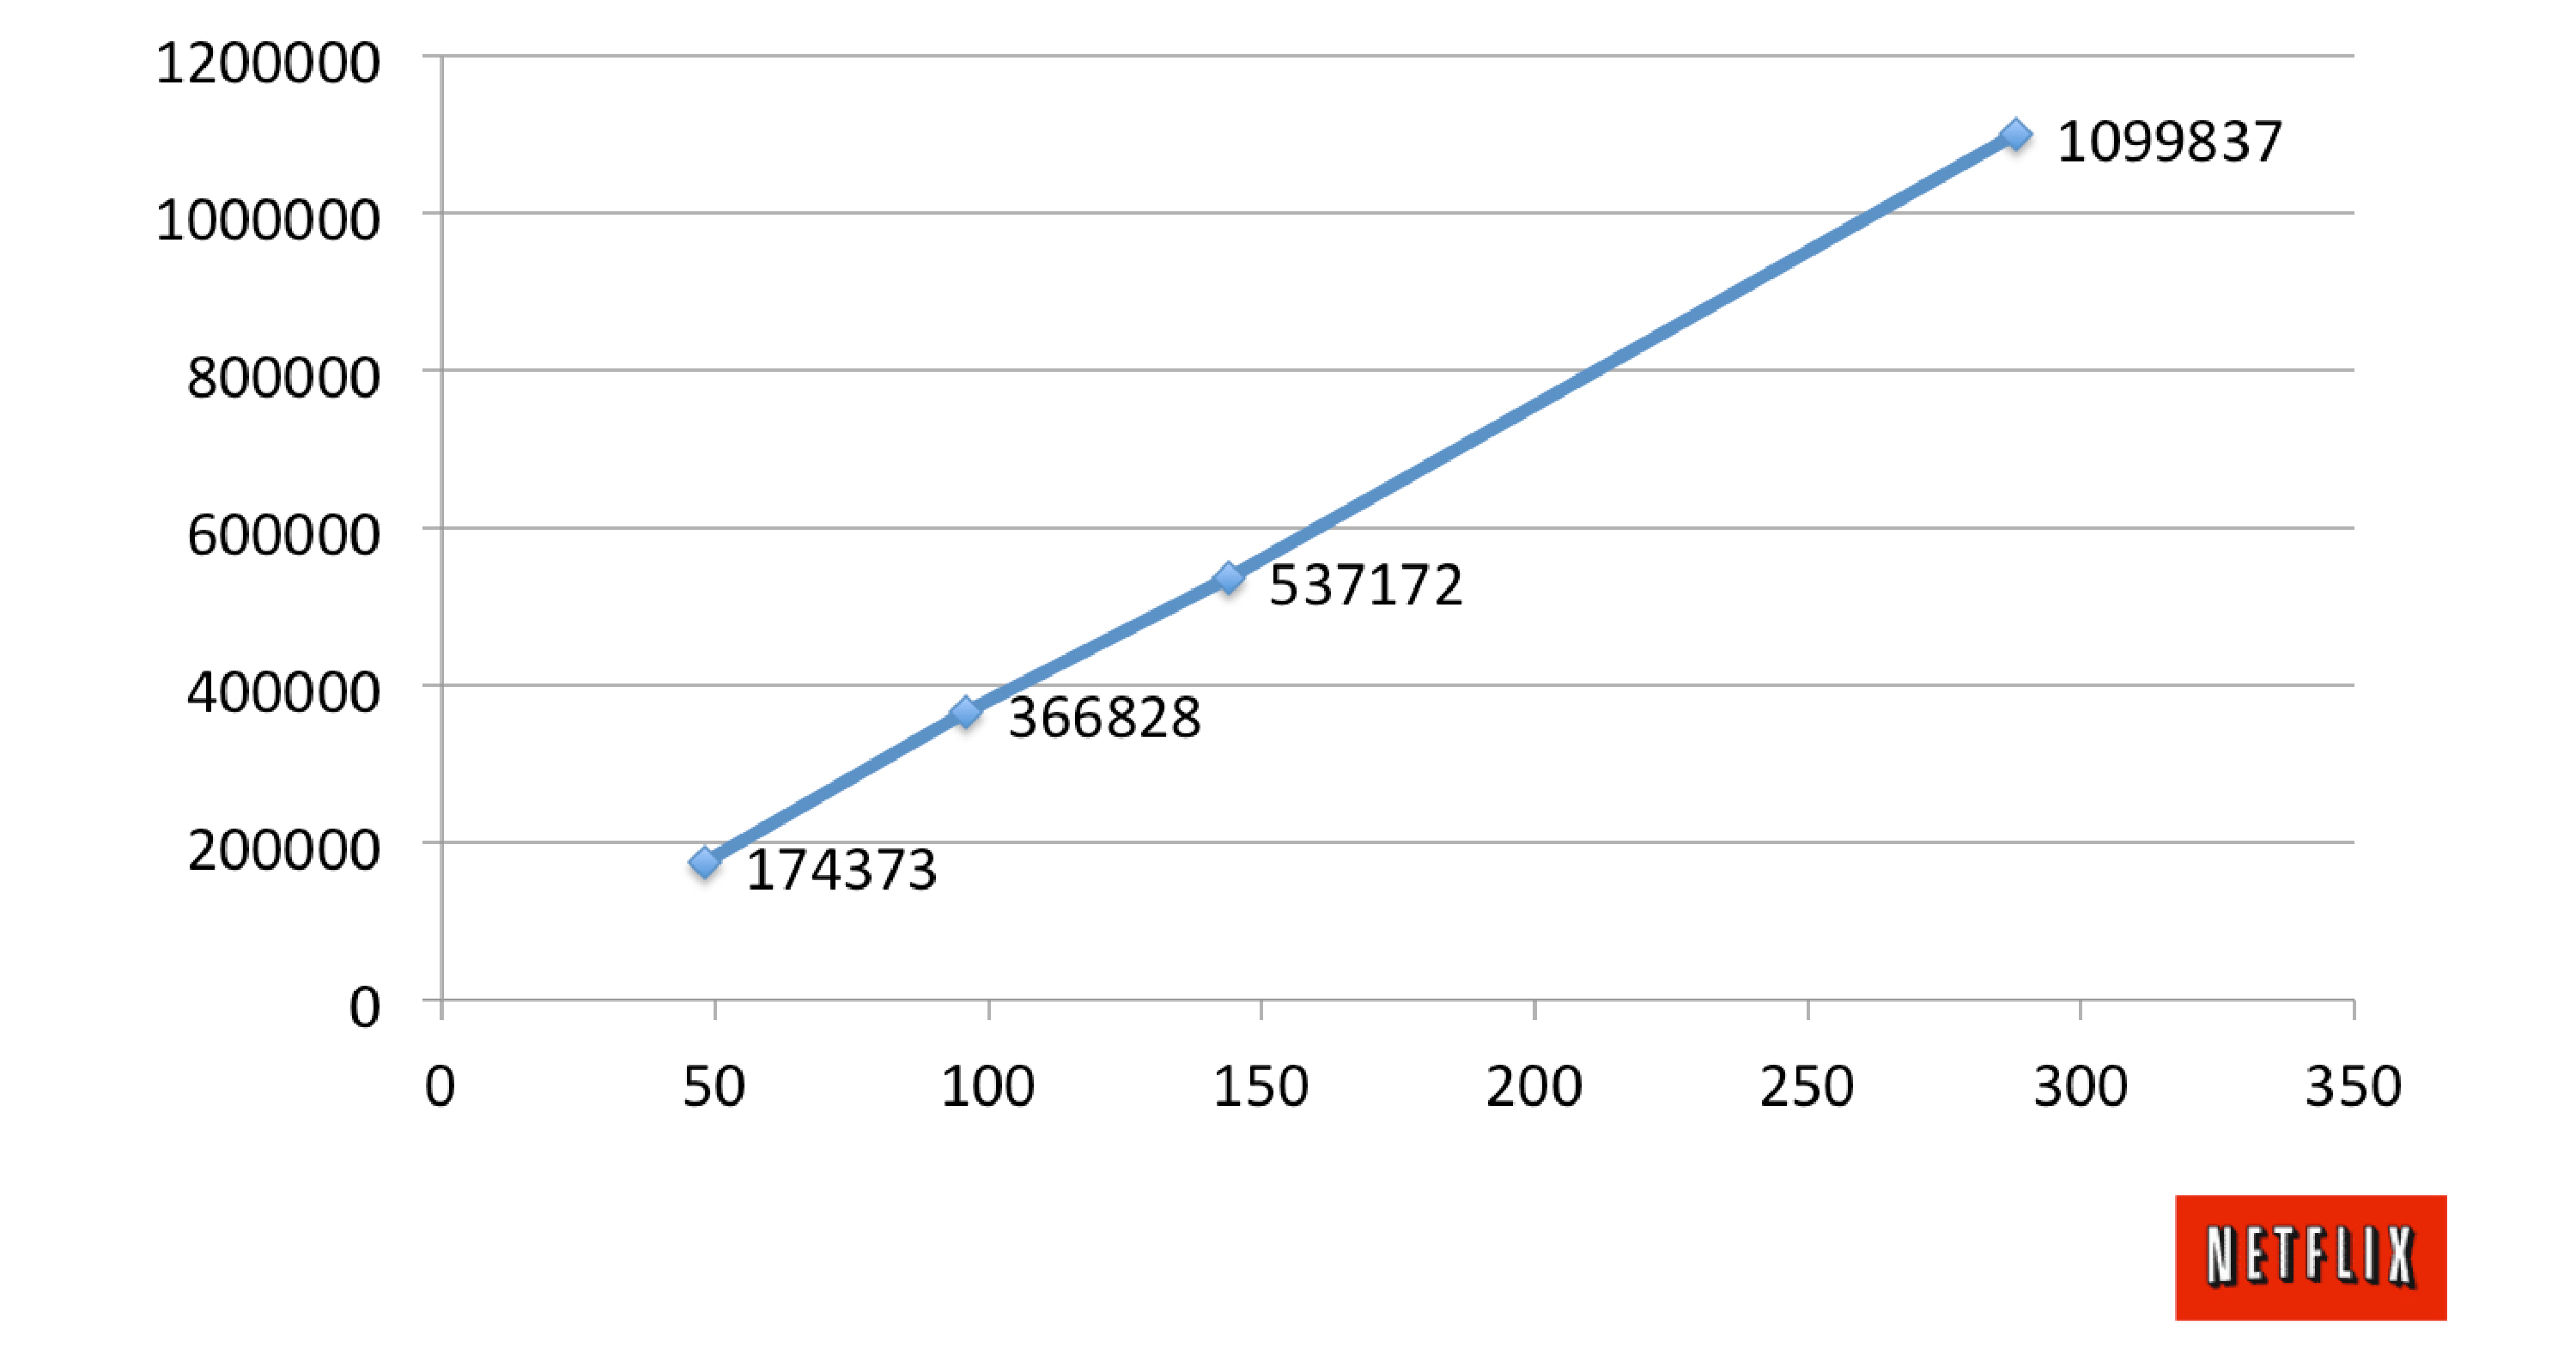
\includegraphics[width=\textwidth]{figure_2.pdf}
  \caption{Netflix experimental data on throughput of its Cassandra database (Client writes/s by node count - Replication Factor=$3$).
  The x-axis is number of nodes; the y-axis is transactions per second. From \cite{cockcroft2011benchmarking}.}
  \label{fig:cassandra_throughput}
\end{figure}

\medskip
Figure \ref{fig:cassandra_throughput} illustrates the throughput properties of Cassandra, a distributed DB technology used by Netflix.
At the bottom left of the plot, we see that $50$ distributed Cassandra nodes handle $174,000$ tps.
Increasing to $300$ nodes gives $1.1$ million transactions per second (tps) \cite{cockcroft2011benchmarking}.
A follow-up study three years later showed a throughput of $1$ million tps with just a few dozen nodes \cite{kalantzis_netflix}.
To emphasize: the throughput of this DB increased as the number of nodes increased. The scaling is linear: $10\times$ more nodes means $(10c)\times$ more throughput, where $0 < c \leq 1$.

Each node also stores data.
Critically, a node only stores a subset of all data, that is, it has partial replication.
In the Netflix example \cite{kalantzis_netflix}, each piece of data has three copies in the system, i.e. a replication factor of three.
Partial replication enables an increase in the number of nodes to increase storage capacity.
Most modern distributed DBs have a linear increase in capacity with the number of nodes, an excellent property.
Additionally, as the number of nodes increases, Cassandra’s latency and network usage does not worsen.
Cassandra can be distributed at scale not only throughout a region, but around the globe.
Contrast this to the Bitcoin blockchain, where capacity does not change as the number of nodes increases.

The scalability properties of distributed DBs like Cassandra make an excellent reference target.

\subsection{Consensus Algorithms in Distributed Databases}
\subsubsection{Introduction}
Cassandra achieves its scale because it avoids scalability-killing decisions like making a full copy of all the data at every node, the baggage of mining, coins, and the like.

What Cassandra does have is a consensus algorithm that uses $2f+1$ processors to tolerate $f$ benign processors\cite{lamport1998part}, which is used to get the distributed data to synchronize.

Synchronizing distributed data was in fact the original motivation for the BG problem.
The problem was first documented in $1980$ by Leslie Lamport and colleagues \cite{pease1980reaching}, and solved two years later, also by Lamport and colleagues.
The solution is the Paxos protocol \cite{lamport1982byzantine} with versions that can tolerate $f$ Byzantine faults using $3f+1$ processors \cite{lamport2011byzantizing, castro2001byzantine}\footnote{Benign faults are system crashes, lost messages, and the like. In systems with benign faults, all nodes are assumed to follow the same protocol.
Byzantine faults include benign faults, but also deviations from the protocol, including lying, collusion, selective non-participation, and other arbitrary behavior.}.

\subsubsection{Paxos Consensus Algorithm}\label{subsec:distributed:paxos}
This section describes the origins of Paxos.
In $1980$, Lamport challenged colleagues with the following question: \quote{Can you implement a distributed database that can tolerate the failure of any number of its processors (possibly all of them) without losing consistency, and that will resume normal behavior when more than half the processors are again working properly?} \cite{lamport_writings}

It was generally assumed at the time that a three-processor system could tolerate one faulty processor.
Lamport’s paper introduced the problem of handling “Byzantine” faults, in which a faulty processor sends inconsistent information to the other processors, which can defeat any traditional three-processor algorithm.
In general, $3f+1$ processors are needed to tolerate $f$ faults.
However, if digital signatures are used, $2f+1$ processors are enough.
This was the first precise statement of the consensus problem \cite{lamport1982byzantine}.

Lamport then set out to prove the problem was impossible to solve \cite{lamport_writings}.
Instead, in a happy accident, he discovered the Paxos algorithm \cite{lamport1998part}.

At the heart of Paxos is a three-phase consensus protocol.
Lamport wrote, “to my knowledge, Paxos contains the first three-phase commit algorithm that is a real algorithm, with a clearly stated correctness condition and a proof of correctness” \cite{lamport_writings}.
Paxos overcame the impossibility result of Fischer et al. \cite{fischer1985impossibility} by using clocks to ensure liveness.

\subsection{Extensions to Paxos Consensus}
The original Paxos could handle arbitrary benign (non-Byzantine) failures such as network delays, packet loss, system crashes and so on.

Several Byzantine fault tolerant systems were designed in the 1980s \cite{wiki_byzantine}, including Draper's FTMP \cite{paulitsch2005coverage}, Honeywell's MMFCS \cite{hopkins1987evolution}, and SRI's SIFT \cite{driscoll1983multi}.

However, those early systems were slow when it came to faults.
Lamport’s “Fast Paxos” \cite{lamport2006fast} and Castro’s “Practical Byzantine Fault Tolerance” (PBFT) \cite{castro2001byzantine} improved upon speed under malicious conditions.
Aardvark \cite{clement2009making} and RBFT \cite{aublin2013rbft} are examples of continued research in speed and reliability.

Paxos is notoriously difficult to understand, and risky to implement.
To address this, Raft \cite{ongaro2014raft} was designed specifically for ease of understanding, and consequent lower implementation risk.
It has a robust variant \cite{copeland2014tangaroa}.

The recent Stellar protocol allows each node to choose which other nodes to trust for validation \cite{mazieres2015stellar}.

\subsection{Usage / Ecosystem}
Mike Burrows of Google (co-inventor of Google’s Chubby, BigTable, and Dapper) has said ``There is only one consensus protocol, and that’s Paxos,'' \cite{robinson2009paxos} and ``all working protocols for asynchronous consensus we have so far encountered have Paxos at their core'' \cite{burrows2006chubby}.
Henry Robinson of Cloudera has said ``all other approaches are just broken versions of Paxo'' and ``it’s clear that a good consensus protocol is surprisingly hard to find.'' \cite{robinson2009paxos}\footnote{An especially interesting statement in light of efforts the Bitcoin community is spending on consensus algorithms.}.

Paxos and its lineage is used at Google, IBM, Microsoft, OpenReplica, VMWare, XtreemFS, Heroku, Ceph, Clustrix, Neo4j, and certainly many more \cite{wiki_paxos}.

\subsection{Replication factor \& blockchain “full nodes”}
A modern distributed DB is designed to appear like a single monolithic DB, but under the hood it distributes storage across a network holding many cheap storage devices.
Each data record is stored redundantly on multiple drives, so if a drive fails the data can still be easily recovered.
If only one disk fails at a time, there only needs to be one backup drive for that data.
The risk can be made arbitrarily small, based on assumptions of how many disks might fail at once.
Modern distributed DBs typically have 3 backups per data object, a replication factor of $3$ \cite{wiki_raid}.

In contrast, Bitcoin has about $6,500$ full nodes \cite{bitcoin2015fees}—a replication factor of $6,500$.
The chance of all nodes going down at once in any given hour (assuming complete independence) is $(1/8760)^{6500}$, or $10^{-25626}$.
The chance of all nodes going down would occur once every $3,000$ billion years. To say this is overkill is to put it mildly.

Of course, hardware failure is not the only reason for lost data.
Attacks against the nodes of the network have a much higher probability of destroying data.
A well-targeted attack to $2$ or $3$ mining pools could just remove $50\%$ of the computing power from the current Bitcoin network, making the network unusable until the next adjustment to POW complexity, which happens about every two weeks.

\subsection{Strengths and Weaknesses}
Let’s review the strengths and weaknesses of DBs that use Paxos-style distributed consensus algorithms.

\medskip
\noindent\textbf{Strengths.} As discussed above, Paxos is a proven consensus algorithm that tolerates benign faults and extensions for Byzantine tolerance have been reported.
It is used by “big data” distributed DBs with the well-documented ability to handle high throughput, low latency, high capacity, efficient network utilization, and any shape of data, including table-like SQL interfaces, object structures of NoSQL DBs, and graph DBs, and they handle replication in a sane fashion.
Derivatives like Raft make distributed consensus systems easier to design and deploy.

\medskip
\noindent\textbf{Weaknesses.} While their technical attributes and performance are impressive, traditional “big data” distributed DBs are not perfect: they are centralized.
They are deployed by a single authority with central control, rather than decentralized control as in blockchains.
This creates a number of failings.
Centralized DBs are:
\begin{itemize}
  \item \textbf{Susceptible to a single point of failure}, where a single node being hacked can be disastrous. This flaw is what lead to hacks at Target, Sony, the U.S. Office of Personnel Management (OPM),and many others \cite{bluestone2014sony_hack, davis2015hacking}.
  \item \textbf{Mutable.} A hacker could change a 5-year-old record without anyone noticing (assuming no additional safeguards in place). For example, this would have prevented police from doctoring evidence in the India exam scandal \cite{sethy2015india_scam}. Such tampering is not possible in blockchains because past transactions cannot be changed or deleted, as each new block contains a “hash” digest of all previous blocks.
  \item \textbf{Not usable by participants with divergent interests} in situations where they do not want to cede control to a single administrator. For example, the risk of losing control of the management of information is one reason that copyright rightsholders in the music industry do not share a single DB.
  \item \textbf{Not designed to stop Sybil attacks}, where one errant node can swamp all the votes in the system.
  \item \textbf{Traditionally without support for the creation and transfer of digital assets} where only the owner of the digital asset, not the administrator of the DB, can transfer the asset.
  \item \textbf{Not typically open to the public} to even read, let alone write. Public openness is important for public utilities. A notable exception is WikiData \cite{wikidata}.
\end{itemize}

\subsection{Fault Tolerance in the BigchainDB System}

Simultaneously preserving the scalability and trustless decentralization of both large-scale databases and decentralized blockchains is the main objective of the BigchainDB system. The following were considered when designing BigchainDB's security measures:

\begin{itemize}
  \item \textbf{Benign faults}: In the BigchainDB setup, nodes communicate through a database which uses a fault-tolerant consensus protocol such as Raft or Paxos. Hence we can assume that if there are $2f + 1$ nodes, $f$ benign-faulty nodes can be tolerated (at any point in time) and each node sees the same order of writes to the database.
  \item \textbf{Byzantine faults}: In order to operate in a trustless network, BigchainDB incorporates measures against malicious or unpredictable behavior of nodes in the system. These include mechanisms for voting upon transaction and block validation. Efforts to achieve full Byzantine tolerance are on the roadmap and will be tested with regular security audits.
  \item \textbf{Sybil Attack}: Deploying BigchainDB in a federation with a high barrier of entry based on trust and reputation discourages the participants from performing an attack of the clones. The DNS system, for example, is living proof of an Internet-scale distributed federation. Appendix \ref{sec:dns} describes how the DNS has successfully run a decentralized Internet-scale database for decades.
\end{itemize}
\section{BigchainDB Description}\label{sec:bigchaindb}

\subsection{Principles}
Rather than trying to scale up blockchain technology, BigchainDB starts with a “big data” distributed database, and adds blockchain characteristics.
It avoids the technology choices that plague Bitcoin, such as full replication.

We built BigchainDB on top of an enterprise-grade distributed DB, from which BigchainDB inherits high throughput, high capacity, a full-featured NoSQL query language, efficient querying, and permissioning. Nodes can be added to increase throughput and capacity.

Since the big data DB has its own built-in consensus algorithm to tolerate benign faults, we exploit that solution directly.
We “get out of the way” of the algorithm to let it decide which transactions to write, and what the block order is.
We disallow private, peer-to-peer communication between the nodes except via the DB’s built-in communication, for great savings in complexity and for reduced security risk\footnote{Though we must vigilantly exercise restraint in design, as intuition is to just get the nodes talking directly!}.
This means that malicious nodes cannot transmit one message to part of the network and different message to other part of the network. Everytime a node ``speaks,'' all the others can listen.

\subsection{High-Level Description}
We focused on adding the following blockchain features to the DB:
\begin{enumerate}
 \item \textbf{Decentralized control}, where “no one” owns or controls a network;
 \item \textbf{Immutability}, where written data is tamper-resistant (“forever”); and
 \item \textbf{The ability to create \& transfer assets} on the network, without reliance on a central entity.
\end{enumerate}

Decentralized control is achieved via a DNS-like federation of nodes with voting permissions.
Other nodes can connect to read and propose transactions; this makes it a super-peer P2P network \cite{ozsu2011principles}.
The voting operates at a layer above the DB’s built-in consensus.
Quorum is a majority of votes.
For speed, each block is written before a quorum of nodes validates and votes on it.
Chainification actually happens at voting time.
Every block has an id equal to the hash of its transactions, timestamp, voters list and public key of its creator-node. It also has a cryptographic signature and a list of votes.
A block doesn't include the hash (id) of the previous block when it first gets written.
Instead, votes get appended to the block over time, and each vote has a ``previous block'' attribute equal to the hash (id) of the block coming before it.
Immutability / tamper-resistance is achieved via several mechanisms: shard replication, reversion of disallowed updates or deletes, regular database backups, and cryptographic signing of all transactions, blocks \& votes.
Any entity with asset-issuance permissions can issue an asset; an asset can only be acquired by new owners if they fulfill its cryptographic conditions.
This means hackers or compromised system admins cannot arbitrarily change data, and there is no single-point-of-failure risk.

\subsection{Architecture}
Figure \ref{fig:bigchaindb_architecture} illustrates the architecture of the BigchainDB system.
The BigchainDB system presents its API to clients as if it is a single blockchain database.
Under the hood, there are actually two distributed databases\footnote{This can be implemented as two databases, or as two tables in the same database. While there is no practical difference, for the sake of clarity we describe it as two separate databases.}, $\mathbf{S}$ (transaction set or “backlog”) and $\mathbf{C}$ (block chain), connected by the BigchainDB Consensus Algorithm (BCA).
The BCA runs on each signing node.
Non-signing clients may connect to BigchainDB; depending on permissions they may be able to read, issue assets, transfer assets, and more; section~\ref{sec:permissioning} explores this more.

\begin{figure}[!ht]
  \centering
  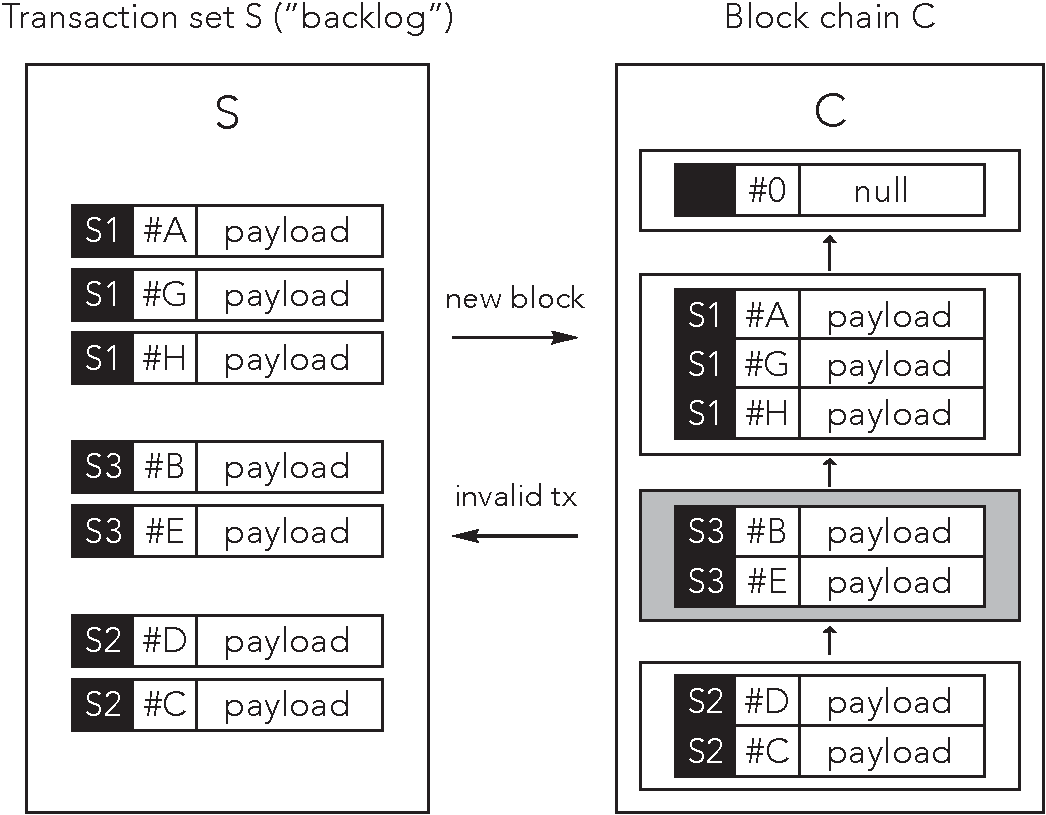
\includegraphics[width=0.7\textwidth]{figure_3.pdf}
  \caption{Architecture of BigchainDB system.
  There are two big data distributed databases: a Transaction Set $\mathbf{S}$ (left) to take in and assign incoming transactions, and a Blockchain $\mathbf{C}$ (right) holding ordered transactions that are “etched into stone”.
  The signing nodes running the BigchainDB Consensus Algorithm update $\mathbf{S}$, $\mathbf{C}$, and the transactions (txs) between them.}
  \label{fig:bigchaindb_architecture}
\end{figure}

Each of the distributed DBs, $\mathbf{S}$ and $\mathbf{C}$, is an off-the-shelf big data DB.
We do not interfere with the internal workings of each DB; in this way, we get to leverage the scalability properties of the DBs, in addition to features like revision control and benefits like battle-tested code.
Each DB is running its own internal Paxos-like consensus algorithm for consistency among the drives.

The first DB holds the “backlog” transactions---an unordered set of transactions~$\mathbf{S}$.
When a transaction comes in, it gets validated by the receiving node and if it's valid (according to that node), then it gets stored in $\mathbf{S}$. (Identical transactions arriving later will be rejected.) The receiving node also randomly assigns the transaction to one of the other nodes.

There are $N$ signing nodes. $\mathbf{S}_k = \{\mathbf{t}_{k,1}, \mathbf{t}_{k,2}, \dots\}$ is the set of transactions assigned to node $\mathbf{k}$.

Node $\mathbf{k}$ running the BigchainDB Consensus Algorithm (BCA) processes transactions from $\mathbf{S}$ as follows: It moves transactions from the unordered set $\mathbf{S}_k$ into an ordered list, creates a block for the transactions, and puts the block into the second database $\mathbf{C}$.
$\mathbf{C}$ is an ordered list of blocks where each block has reference to a parent block and its data, that is, a blockchain.

A signing node can vote on whether it considers a block \textsf{\textit{valid}} or \textsf{\textit{invalid}}. To decide, the signing node checks the validity of every transaction in the block, and if it finds an invalid transaction, then the signing node votes that the block is \textsf{\textit{invalid}}.
If the signing node finds no invalid transactions, then it votes that the block is \textsf{\textit{valid}}.

Each block starts out as \textsf{\textit{undecided}}, with no votes from signing nodes.
Once there is majority of positive (\textsf{\textit{valid}}) votes for a block, or a majority of negative (\textsf{\textit{invalid}}) votes, the block goes from \textsf{\textit{undecided}} to \textsf{\textit{decided\_valid}} or \textsf{\textit{decided\_invalid}}, respectively, and voting on the block stops.
Once it is decided, it can be treated as “etched into stone.” This process is similar to the idea of multiple confirmations in Bitcoin blockchain.

A block $\mathbf{B}$ in the blockchain has an ID, timestamp, the actual transactions, and vote information. Section \ref{subsec:bigchaindb:models} describes block, transaction, and voting models precisely.

\subsection{Behavioral Description}
This section examines the flow of transactions from a client to a given server node.
Each server node has its own view of the transaction backlog $\mathbf{S}$, and the chain $\mathbf{C}$.

\begin{figure}[!ht]
  \centering
  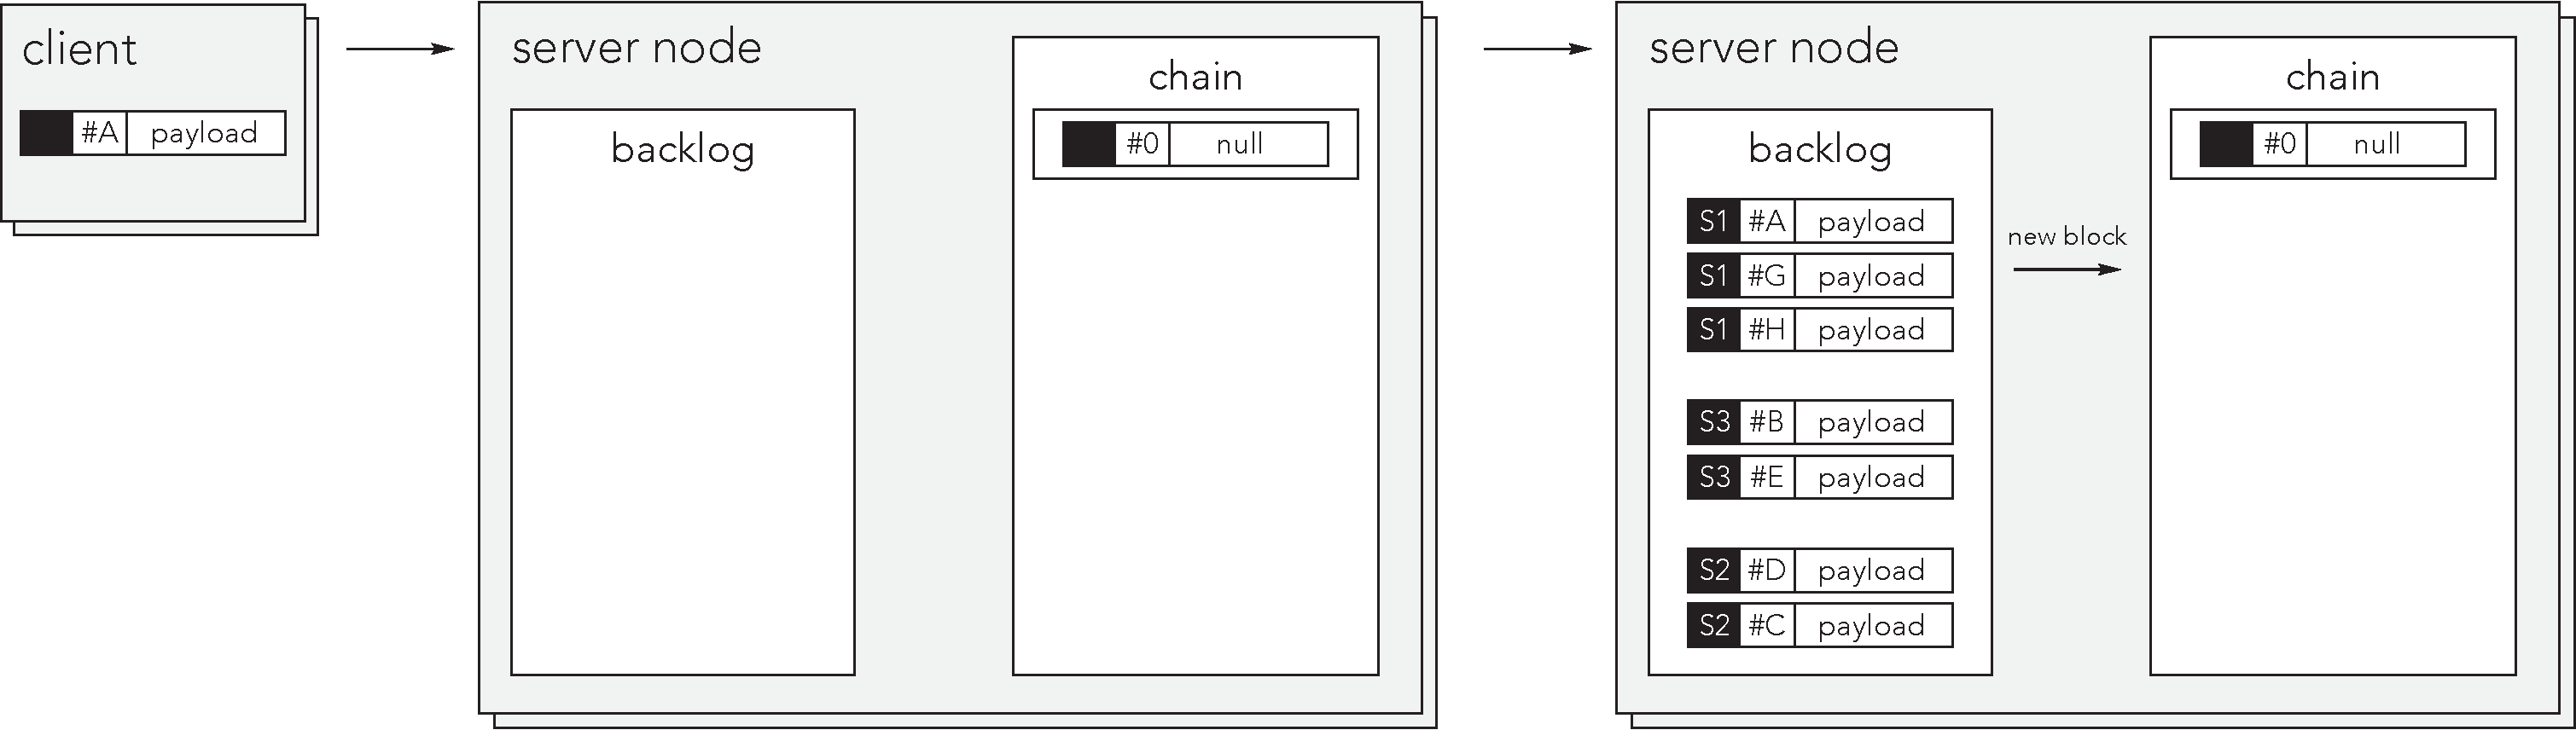
\includegraphics[width=\textwidth]{figure_4.pdf}
  \caption{\textit{Left:} The backlog $\mathbf{S}$ starts empty and the chain $\mathbf{C}$ starts with only a genesis block.
  \textit{Right:} Clients have inserted transactions into backlog $\mathbf{S}$ and assigned to nodes 1, 3, and 2.}
  \label{fig:bigchaindb_architecture_step1}
\end{figure}

Figure \ref{fig:bigchaindb_architecture_step1} and subsequent figures illustrate the high-level architecture where each card is a physical machine.
The client machines are on the left\footnote{In some images, we truncate the illustration of the client, for brevity.}.
Clients are connected to the BigchainDB server node(s) (voting node), shown on the right. Any client may send transactions to any BigchainDB server node.

In Figure \ref{fig:bigchaindb_architecture_step1} left, one client has a transaction with ID \textsf{$\#$A}, and a payload.
BigchainDB’s backlog $\mathbf{S}$ is empty; and the chain $\mathbf{C}$ is empty except for a genesis block with a null transaction.
Other clients also have transactions that they transmit to server nodes.

When a client submits a transaction, the receiving node assigns it to one of the federation nodes, possibly itself, and stores it in the backlog~$\mathbf{S}$.
Figure~\ref{fig:bigchaindb_architecture_step1} right illustrates an example state.
We see that node~1 is assigned three transactions, having IDs of \textsf{$\#$A}, \textsf{$\#$G}, and \textsf{$\#$H}.
Node~3 is assigned transactions with IDs~\textsf{$\#$B} and \textsf{$\#$E}.
Node~2 is assigned transactions~\textsf{$\#$D} and \textsf{$\#$C}. Nothing has been stored on the chain~$\mathbf{C}$ yet (besides the genesis block).

\begin{figure}[!ht]
  \centering
  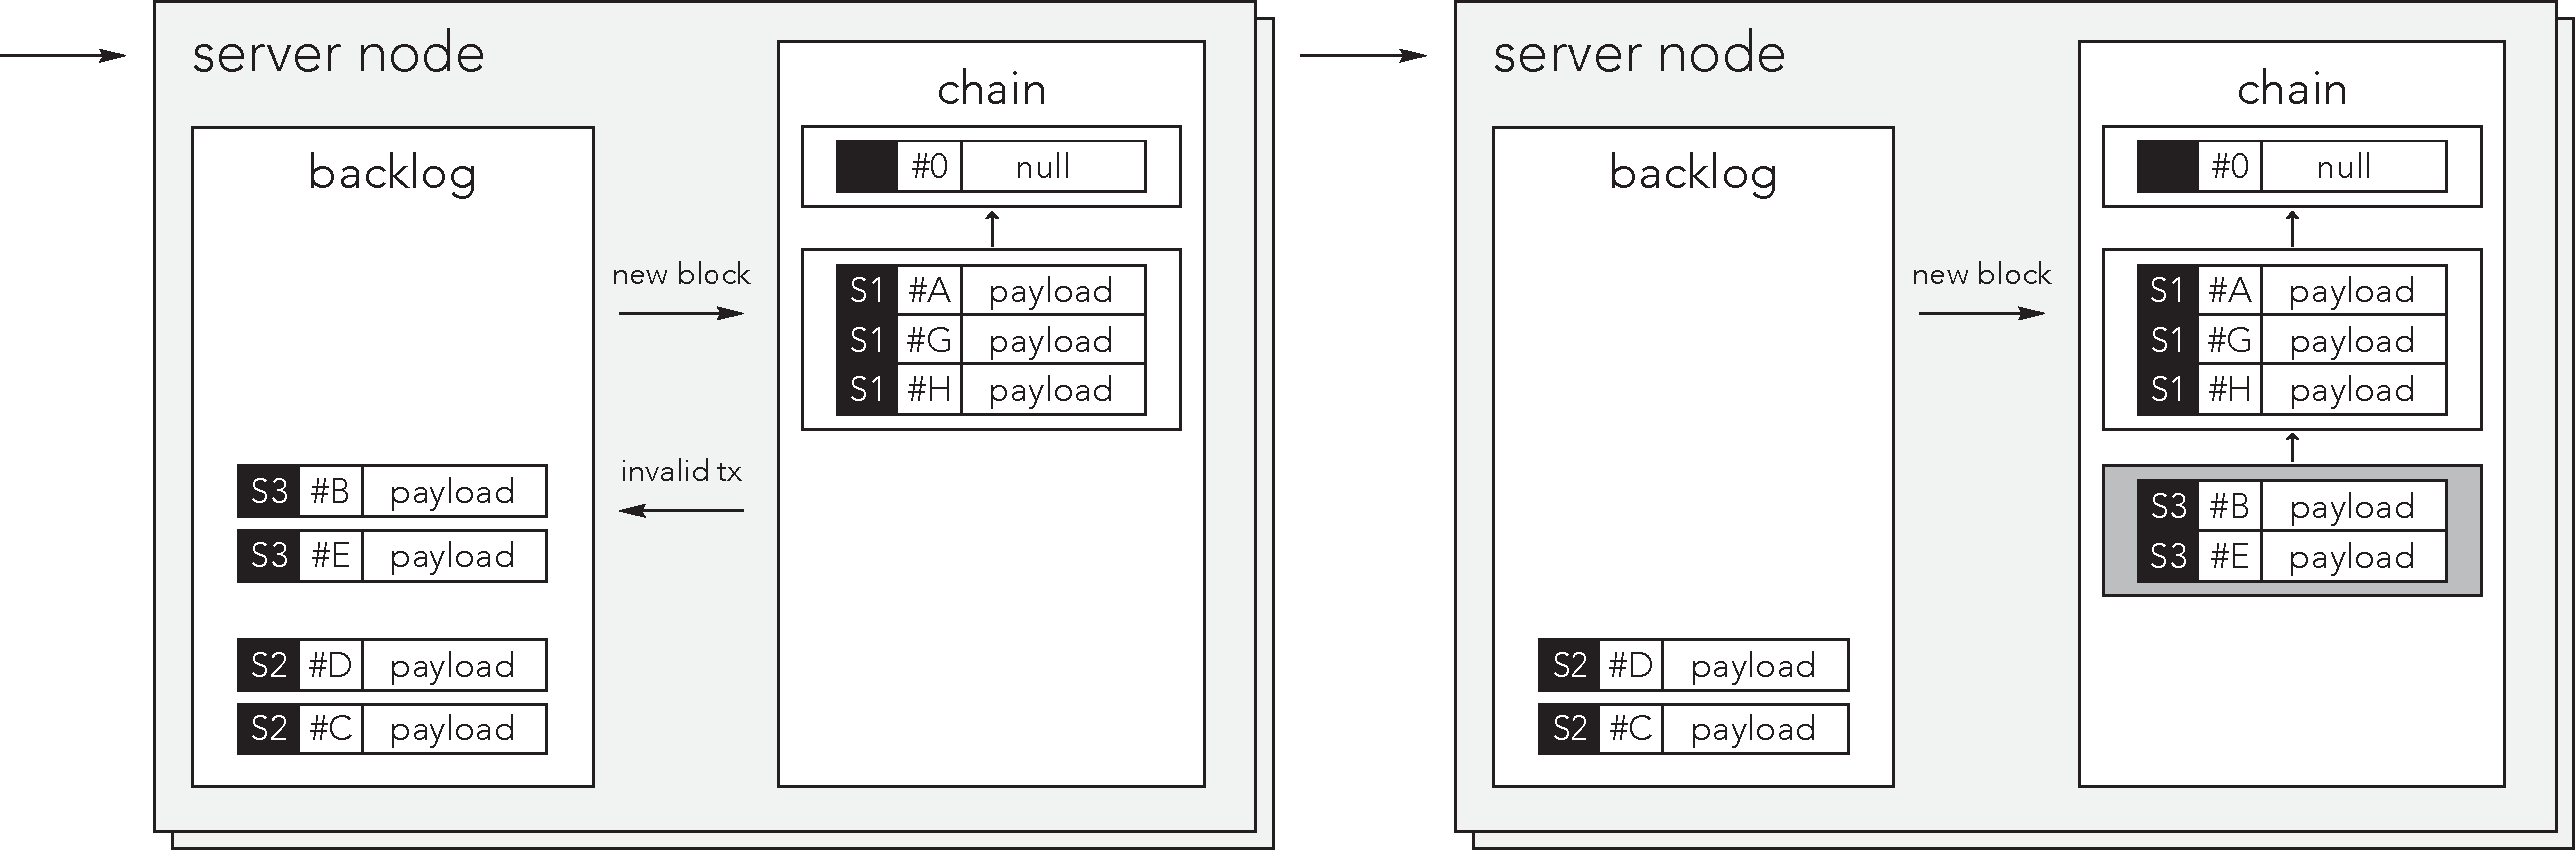
\includegraphics[width=\textwidth]{figure_5.pdf}
  \caption{\textit{Left:} Node 1 has moved its assigned transactions from backlog $\mathbf{S}$ to chain $\mathbf{C}$.
  \textit{Right:} Node 3 has processed its assigned transactions too.}
  \label{fig:bigchaindb_architecture_step2}
\end{figure}

Figure \ref{fig:bigchaindb_architecture_step2} left shows a state where Node 1 has processed all the transactions assigned to it.
It has taken the transactions \textsf{$\#$A}, \textsf{$\#$G}, and \textsf{$\#$H} from the backlog $\mathbf{S}$, created a block to hold them, then written the block onto the chain $\mathbf{C}$.
The block points to $\mathbf{C}$’s previous block.

Figure \ref{fig:bigchaindb_architecture_step2} right shows where Node 3 has processed all of its assigned transactions too, and therefore written them as a block in chain $\mathbf{C}$.

When a block is first written to $\mathbf{C}$, it starts off as \textsf{\textsf{\textit{undecided}}}.
Each server node may vote positively (for) or negatively (against) a block.
A block should only be voted positively if all previous blocks are not \textsf{\textit{undecided}}, and all transactions in the block itself are valid.
As soon as there is a majority of positive votes for a block, or a majority of negative votes, the block goes from \textsf{\textit{undecided}} to \textsf{\textit{decided\_valid}} or \textsf{\textit{decided\_invalid}}, respectively.

In this example, the block created by Node 1 gets voted on, and becomes \textsf{\textit{decided\_valid}}.
Then, the block from node 3 gets voted on, and becomes \textsf{\textit{decided\_invalid}}.
In Figure \ref{fig:bigchaindb_architecture_step2} right, we depict the distinction as a clear background for \textsf{\textit{decided\_valid}}, versus a shaded background for \textsf{\textit{decided\_invalid}}.)

\begin{figure}[!ht]
  \centering
  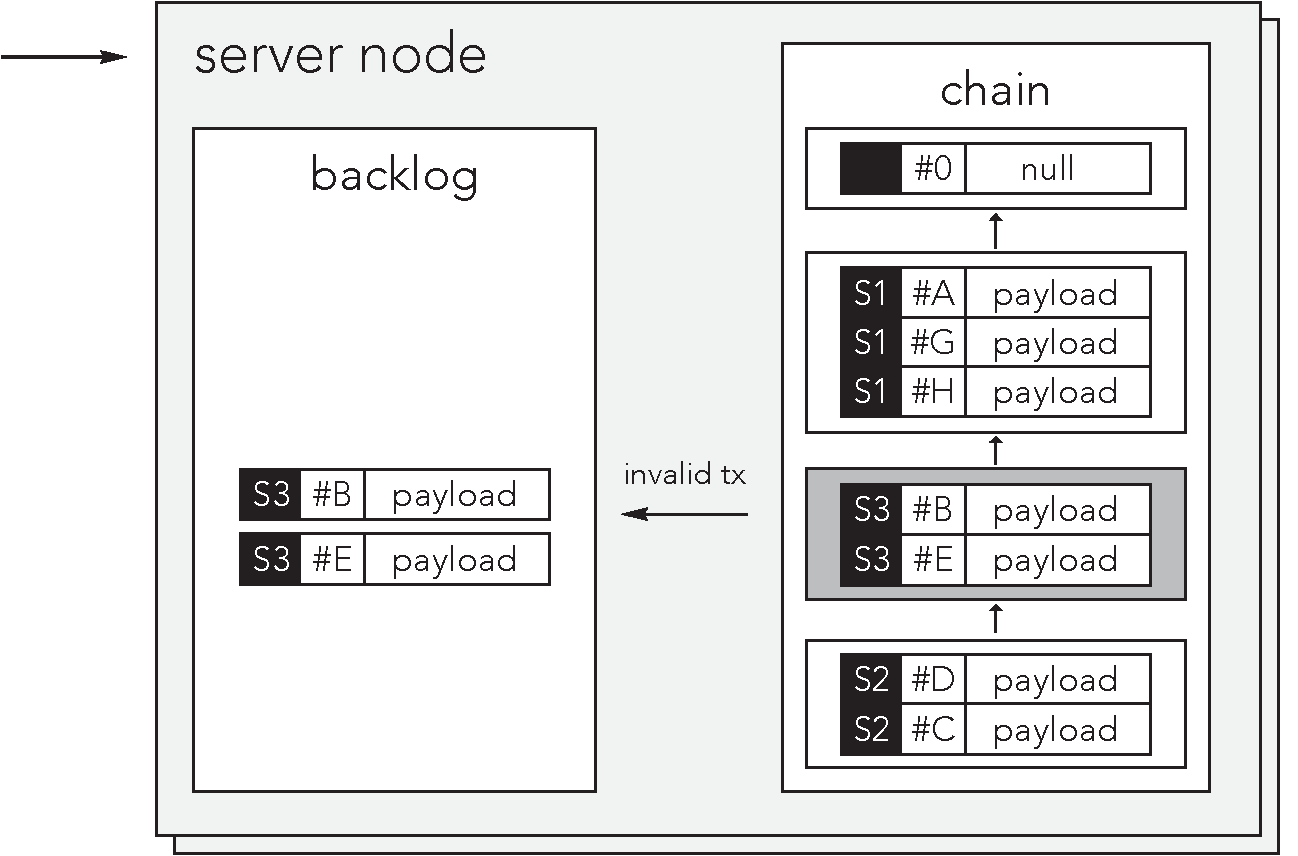
\includegraphics[width=0.5\textwidth]{figure_6.pdf}
  \caption{Transactions from an invalid block (on right, shaded) get re-inserted into backlog $\mathbf{S}$ for re-consideration.}
  \label{fig:bigchaindb_architecture_step3}
\end{figure}

While the overall block was considered invalid, some of the transactions in the invalid block may have actually been valid, and so BigchainDB gives them another chance.
Figure \ref{fig:bigchaindb_architecture_step3} illustrates how: transactions \textsf{$\#$B} and \textsf{$\#$E} get re-inserted into backlog $\mathbf{S}$ for new consideration.
Figure \ref{fig:bigchaindb_architecture_step3} also shows how BigchainDB approaches storage of invalid blocks.
There’s a block in the chain $\mathbf{C}$ that is invalid.
However, BigchainDB doesn’t remove the block; there’s no need, as the block is already marked invalid, disk space is not a problem, and it’s faster and simpler to keep all blocks there.
Similarly, voting doesn’t stop after a block becomes decided, because it’s faster for each node to simply vote than the extra step to check whether voting is necessary.

\begin{figure}[!ht]
  \centering
  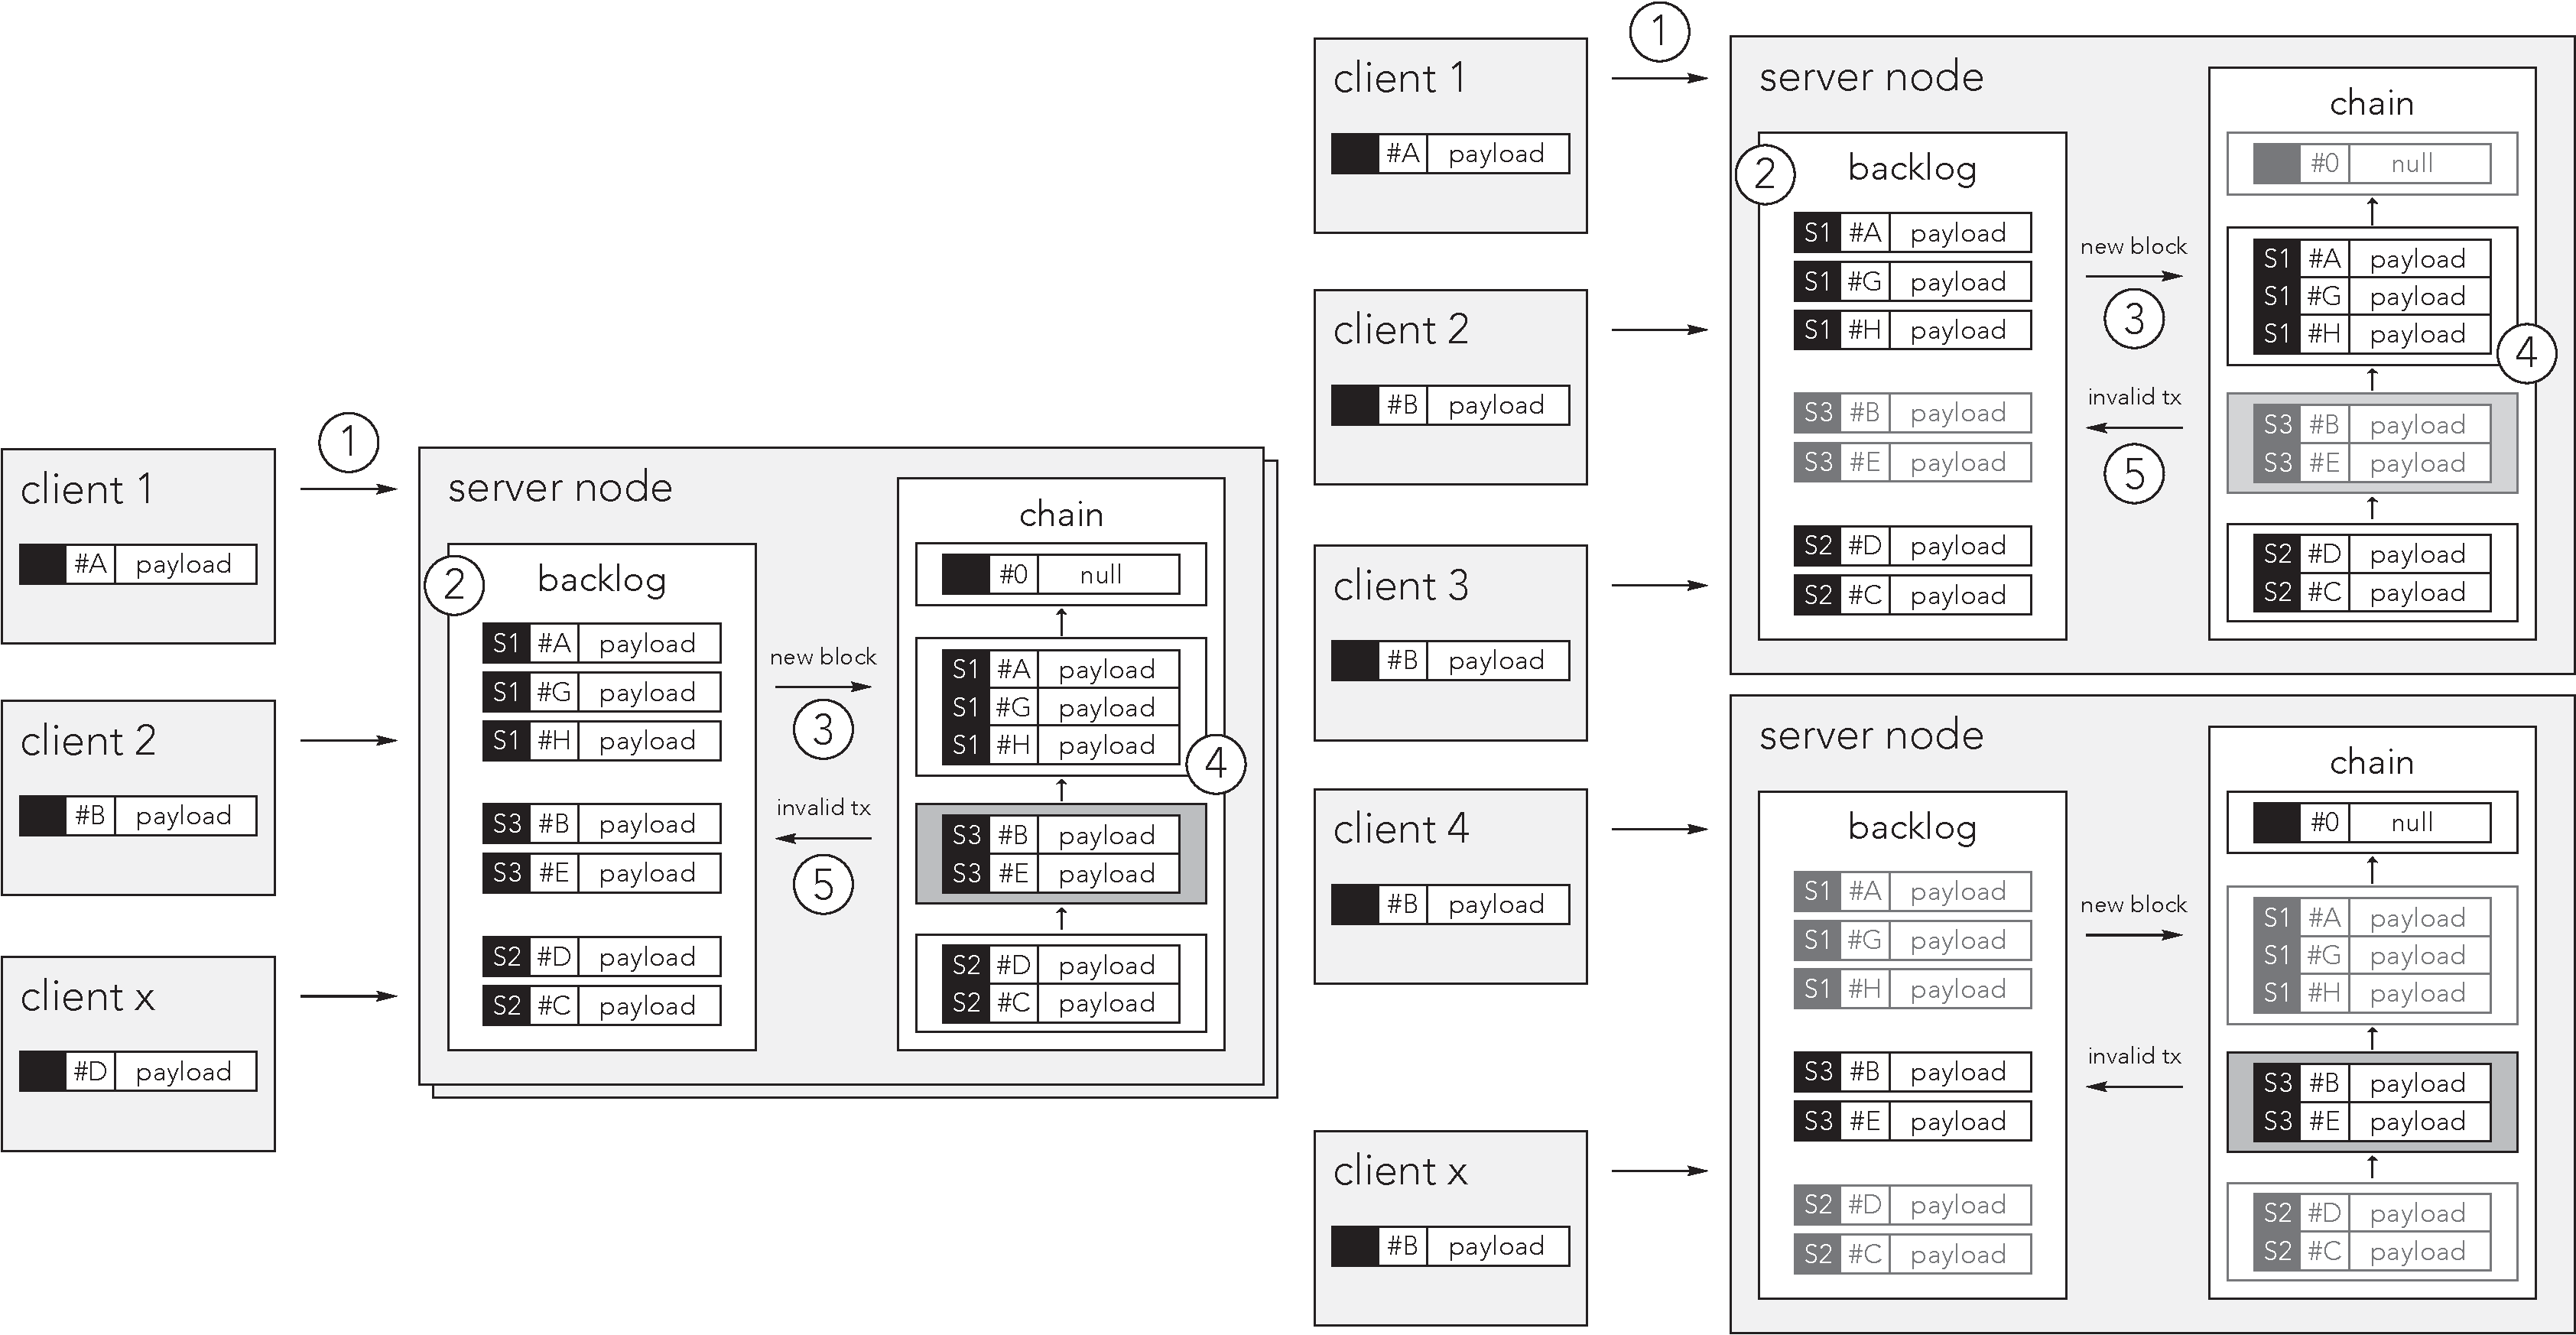
\includegraphics[width=\textwidth]{figure_7.pdf}
  \caption{\textit{Left:} More than one client may talk to a given node.
  \textit{Right:} there are multiple nodes. Typically, a client connects to just one node (an arbitrarily picked one).}
  \label{fig:bigchaindb_architecture_sharding}
\end{figure}

Figure \ref{fig:bigchaindb_architecture_sharding} emphasizes how multiple machines are configured.
Figure \ref{fig:bigchaindb_architecture_sharding} left shows that more than one client may talk to a given node.
Figure \ref{fig:bigchaindb_architecture_sharding} right shows that there is more than one node, though each node has a view into the backlog $\mathbf{S}$ and the chain $\mathbf{C}$.


\subsection{Data Models}\label{subsec:bigchaindb:models}
\subsubsection{Transaction Model}
Transactions are the most basic kind of record stored by BigchainDB. There are two kinds: creation transactions and transfer transactions. A creation transaction initiates the records of an asset\footnote{While we use the word ``asset,'' BigchainDB can be used to record information about things more general than assets.} in BigchainDB, including some description of what it is, a list of its initial owners, and the conditions that must be fulfilled by anyone wishing to transfer it. A transfer transaction transfers ownership of the asset to new owners, and assigns new spending conditions.

A transaction is represented by a JSON document with the following structure:

\begin{lstlisting}[style=json]
{
    "id": "<hash of transaction, excluding signatures>",
    "version": "<version number of the transaction model>",
    "transaction": {
        "fulfillments": ["<list of fulfillments>"],
        "conditions": ["<list of conditions>"],
        "operation": "<string>",
        "timestamp": "<timestamp from client>",
        "data": {
            "hash": "<hash of payload>",
            "payload": "<any JSON document>"
        }
    }
}
\end{lstlisting}

where:

\begin{itemize}
 \item $\mathtt{id}$: The hash of everything inside the serialized $\mathtt{transaction}$ body (see below), with one wrinkle: for each fulfillment in $\mathtt{fulfillments}$, $\mathtt{fulfillment}$ is set to $\mathtt{null}$. The $\mathtt{id}$ is also the database primary key.
 \item $\mathtt{version}$: Version number of the transaction model, so that software can support different transaction models.
 \item $\mathtt{fulfillments}$: List of fulfillments. Each fulfillment contains a pointer to an unspent asset and a crypto-fulfillment that satisfies a spending condition set on the unspent asset. A fulfillment is usually a signature proving the ownership of the asset.
 \item $\mathtt{conditions}$: List of conditions. Each condition is a crypto-condition that needs to be fulfilled by by a transfer transaction in order to transfer ownership to new owners.
 \item $\mathtt{operation}$:  String representation of the operation being performed (currently either ``CREATE'' or ``TRANSFER''). It determines how the transaction should be validated.
 \item $\mathtt{timestamp}$: Time of creation of the transaction in UTC. It's provided by the client.
 \item $\mathtt{hash}$: The hash of the serialized $\mathtt{payload}$.
 \item $\mathtt{payload}$: Can be any JSON document. It may be empty in the case of a transfer transaction.
\end{itemize}

Full explanations of transactions, conditions and fulfillments are beyond the scope of this paper; see the BigchainDB Documentation \cite{bigchaindb_doc} and the Interledger Protocol \cite{thomas2015interledger} for additional details.


\subsubsection{Block Model}
A block is represented by a JSON document with the following structure:

\begin{lstlisting}[style=json]
{
    "id": "<hash of block>",
    "block": {
        "timestamp": "<block-creation timestamp>",
        "transactions": ["<list of transactions>"],
        "node_pubkey": "<public key of the node creating the block>",
        "voters": ["<list of federation nodes public keys>"]
    },
    "signature": "<signature of block>",
    "votes": ["<list of votes>"]
}
\end{lstlisting}

\begin{itemize}
  \item $\mathtt{id}$: The hash of the serialized $\mathtt{block}$. This is also a database primary key; that's how we ensure that all blocks are unique.
  \item $\mathtt{block}$:
    \begin{itemize}
      \item $\mathtt{timestamp}$: Timestamp when the block was created. It's provided by the node that created the block.
      \item $\mathtt{transactions}$: A list of the transactions included in the block.
      \item $\mathtt{node\_pubkey}$: The public key of the node that created the block.
      \item $\mathtt{voters}$: A list of public keys of federation nodes. Since the size of the 
      federation may change over time, this will tell us how many nodes existed
      in the federation when the block was created, so that at a later point in
      time we can check that the block received the correct number of votes.
    \end{itemize}
  \item $\mathtt{signature}$: Signature of the block by the node that created the block. (To create the signature, the node serializes the block contents and signs that with its private key.)
  \item $\mathtt{votes}$: Initially an empty list. New votes are appended as they come in from the nodes.
\end{itemize}


\subsubsection{Vote Model}
Each node must generate a vote for each block, to be appended to that block's $\mathtt{votes}$ list. A vote has the following structure:

\begin{lstlisting}[style=json]
{
    "node_pubkey": "<the public key of the voting node>",
    "vote": {
        "voting_for_block": "<id of the block the node is voting for>",
        "previous_block": "<id of the block previous to this one>",
        "is_block_valid": "<true|false>",
        "invalid_reason": "<None|DOUBLE_SPEND|TRANSACTIONS_HASH_MISMATCH|NODES_PUBKEYS_MISMATCH",
        "timestamp": "<timestamp of the voting action>"
    },
    "signature": "<signature of vote>"
}
\end{lstlisting}


\subsection{Block Validity and Blockchain Pipelining}

\begin{figure}[!ht]
  \centering
  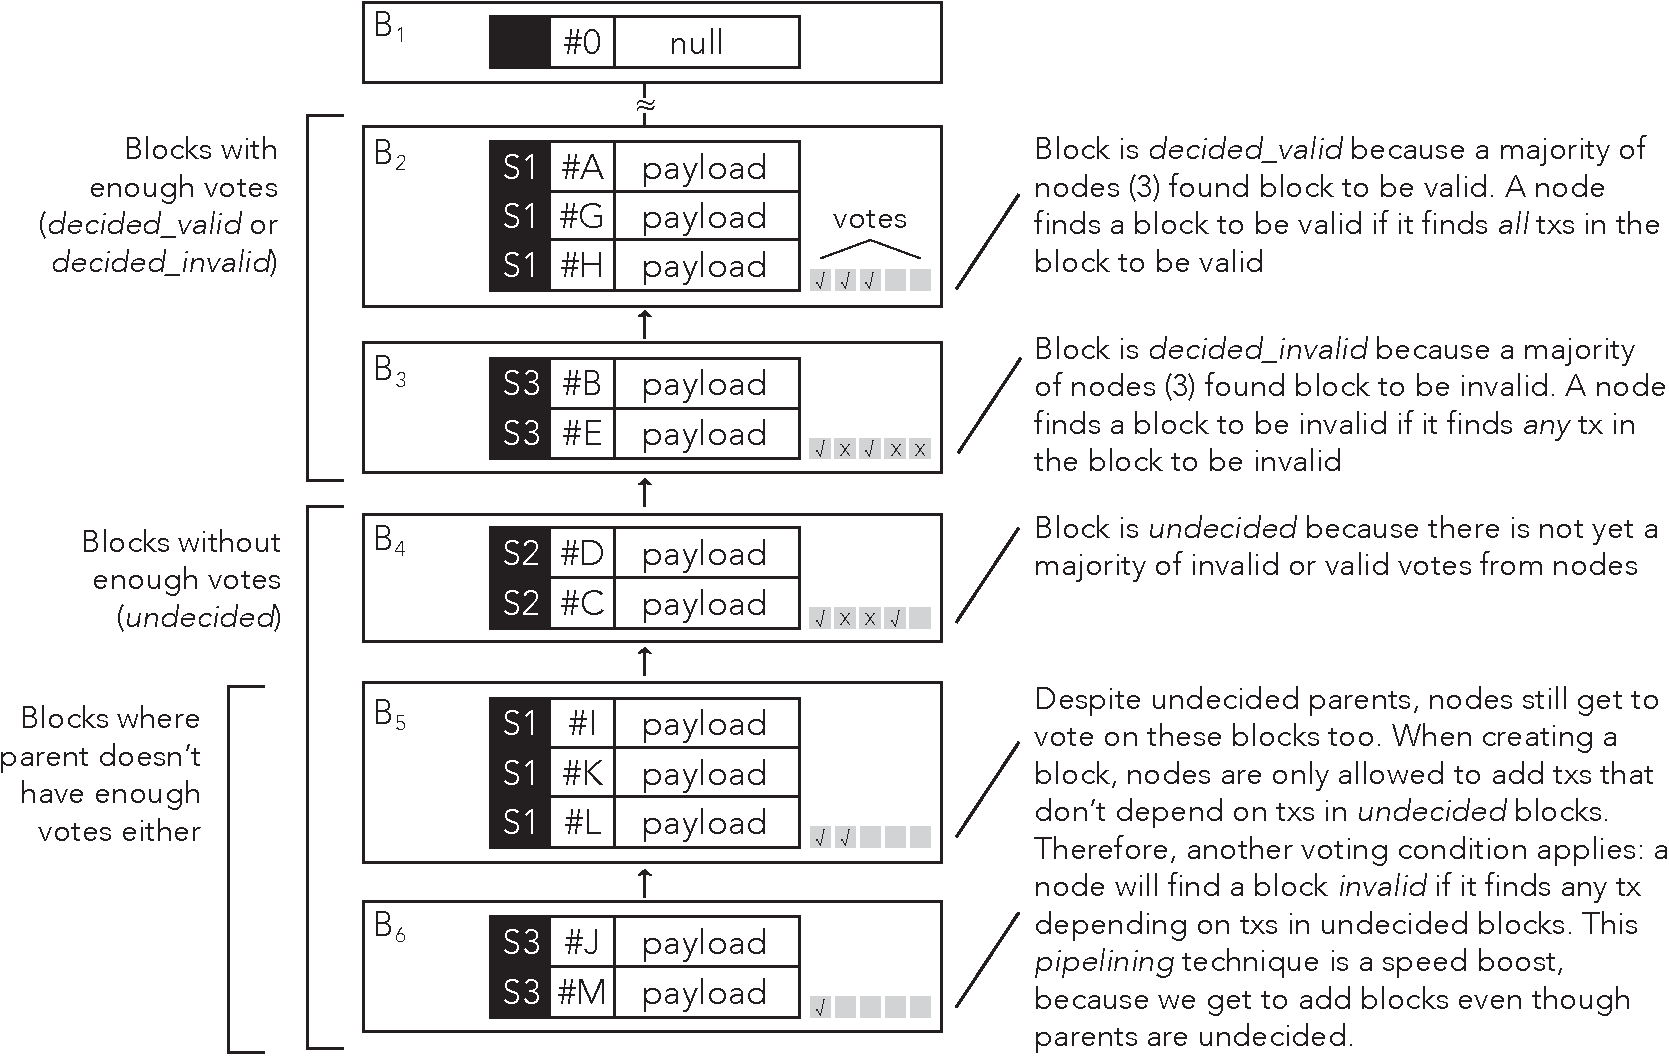
\includegraphics[width=\textwidth]{figure_8.pdf}
  \caption{Pipelining in the BigchainDB blockchain $\mathbf{C}$.
  Votes accumulate on each block.
  Blocks can continue to accumulate on the blockchain, even though their parents, grandparents, etc. may be undecided.
  The key is that when adding a new block, we can include transactions that do not depend on transactions in undecided blocks.}
  \label{fig:bigchaindb_chain_pipelining}
\end{figure}

Figure \ref{fig:bigchaindb_chain_pipelining} shows an example of a blockchain $\mathbf{C}$.
Block $\mathbf{B}_1$ is the genesis block with a null transaction.

Blocks are written to $\mathbf{C}$ in an order decided by the underlying DB.
This means that when a signing node inserts a block into $\mathbf{C}$, it cannot provide a vote at the same time (because a vote includes a reference to the previous block, but the previous block isn't known yet).
Only after the write is fully-committed does the block order become clear. 

Nodes vote on blocks after order becomes clear.
When a block is created, it starts off \textsf{\textit{undecided}}.
As soon as there is majority of positive votes for a block, or a majority of negative votes, the block goes from \textsf{\textit{undecided}} to \textsf{\textit{decided\_valid}} or \textsf{\textit{decided\_invalid}}, respectively.

Note that, unlike a typical block chain, the BigchainDB block model doesn't have a reference to the previous block.
Instead, it has a list of votes, and each vote has a reference to the previous block (i.e.~the block that the voting node considered the previous block, based on its view of the changefeed). We say that ``chainification happens at \textit{voting} time.''

Normally, all votes will reference the same previous block, but it's possible that different votes may claim that different blocks are the previous block. This can happen, for example, if a node goes down. When it comes back up, there's no reliable way to recover the order of the new blocks it missed while down. What should it put as the id/hash of the previous block? We will experiment with various options (e.g.~an id/hash value of ``null'' or the same id/hash as the majority of other votes).

If a node goes down, it won't accumulate a long list of new blocks that it must vote on when it comes back up. That's because the list of expected voters (nodes) for a block is set when that block is created. If a node is down when a block is created, then it won't be put on the list of expected voters for that block.

Block $\mathbf{B}_2$ has received three votes of five possible.
In this example, all three votes are positive.
Since the majority of nodes voted that the block is \textsf{\textit{valid}}, the block is considered \textsf{\textit{decided\_valid}}.

Block $\mathbf{B}_3$ has received five votes of five possible.
There was a positive vote, then negative, then positive, then two more negative votes.
Since the majority of nodes voted that the block is \textsf{\textit{invalid}}, the block is considered \textsf{\textit{decided\_invalid}}.
This block can stay in the chain because all the votes show that it is invalid.
It will be ignored when validating future transactions.
By keeping the block in place, we can quickly progress the chain to child blocks.

Block $\mathbf{B}_4$ is \textsf{\textit{undecided}} because it does not yet have a majority of invalid or valid votes from nodes.
Voting on $\mathbf{B}_4$ continues.

It is crucial that despite $\mathbf{B}_4$ being \textsf{\textit{undecided}}, it still has a child block $\mathbf{B}_5$.
This is possible because the DB’s built-in consensus algorithm determines the order of the blocks, and we have logically separated writing blocks from voting.
“Forking” is not a risk as it is not even in the vocabulary of the DB, let alone supported in code.
The reason is that every node is working on the same blockchain (instead of every node working on their own replica of the blockchain which may be different from the other nodes) and every node communicates through the database which is basically an open broadcast channel (instead of communicating individually with each node).
Because of this, any node can try to add a block, but only one becomes the child to $\mathbf{B}_4$; the rest follow according to the built-in consensus algorithm.
It is a single railroad track where the location of the next plank is based on previous planks.
We do not have to stop at adding a single plank after an undecided block—we can keep aggressively laying track, such as block $\mathbf{B}_6$ in the figure.

When there are undecided parent blocks, we need to do one more thing to prevent double-spending: any transaction put into a new block must not depend on transactions in an undecided block.
For example, inputs of a new transaction must not be in inputs of any undecided blocks.
This is enforced in two ways: when creating new blocks on undecided blocks, such double-spend transactions are not allowed, and when voting, any block containing such transactions is voted invalid.

We call this “blockchain pipelining” because this behavior is reminiscent of pipelining in microprocessors.
There, the microprocessor starts executing several possible instructions at once.
Once the microprocessor has worked out the proper order for the instructions, it collates the results as output and ignores useless results.
As with microprocessor pipelining, blockchain pipelining gives significant speed benefits.

\subsection{BigchainDB Consensus Algorithm (BCA)}

The BigChainDB Consensus Algorithm (BCA) is a state machine that runs on each “signing” node (server).
This section outlines the BCA using Python-like pseudocode.\footnote{The actual code will be open source, so if you’re curious about implementation details, you can read that.}

\subsubsection{Main Loop}

Before starting the $\mathtt{mainLoop()}$ on each signing node, the databases $\mathbf{S}$ and $\mathbf{C}$ must be created and initialized.
One of the initialization steps is to write a genesis block to $\mathbf{C}$.

Listing \ref{lst:bca} has high-level pseudocode for the BCA.
It shows the $\mathtt{mainLoop()}$ running on signing node $\mathbf{k}$.
Every signing node runs the same $\mathtt{mainLoop()}$.

Line $\mathtt{4}$ emphasizes that there is equal access by all the nodes to the databases $\mathbf{S}$ and $\mathbf{C}$. 
The BCA operates by moving data from transaction set $\mathbf{S}$ to blockchain $\mathbf{C}$, and occasionally in the other direction as well.

\begin{minipage}{\linewidth}
  \begin{lstlisting}[caption={BigchainDB Consensus Algorithm. This algorithm runs on every signing node.}, label={lst:bca}, style=python]
  def mainLoop(): # Pseudocode for signing node k 
    # Assume S and C exist and are initialized,
    # and C contains a genesis block. 
    global S, C # tx set and blockchain globally visible
    while True: 
      S = assignTransactions(S, k) 
      Sk, C = addBlock(Sk, C, k) 
      C = voteOnBlocks(C, k)
  \end{lstlisting}
\end{minipage}

Line $\mathtt{5}$ is the start of the main loop. All remaining pseudocode is part of this loop, which runs continuously until the node is shut down.

Line $\mathtt{6}$ accepts transactions into $\mathbf{S}$ and assigns them to nodes, line $\mathtt{7}$ moves unordered transactions from $\mathbf{S}$ into ordered, grouped-by-block transactions in $\mathbf{C}$, and line $\mathtt{8}$ is where the node votes on undecided blocks.

\begin{minipage}{\linewidth}
  \begin{lstlisting}[caption={Parallel version of BigchainDB Consensus Algorithm.}, label={lst:bca_parallel}, style=python]
  def mainLoopParallel():
    start => 1 assignTransactionLoop() processes 
    start => 1 addBlockLoop() processes 
    start => 1 voteLoop() processes
    
  def assignTransactionLoop():
    while True:
      S = assignTransactions(S, k)
  
  def addBlockLoop():
    while True:
      Sk, C = addBlock(Sk, C, k)
  
  def voteLoop():
    while True:
      C = voteOnBlocks(C, k)
  \end{lstlisting}
\end{minipage}

The pseudocode of Listing \ref{lst:bca} is written as if there is a single process, but each major step can actually be a separate, independent process.
In fact, there may be multiple processes doing each step; this helps performance tremendously.
Listing \ref{lst:bca_parallel} shows the pseudocode.

\subsubsection{Assigning Transactions}

\medskip
\noindent Listing \ref{lst:bca_tx_routines} algorithms are for assigning transactions, as follows:

Listing \ref{lst:bca_tx_routines} $\mathtt{assignTransactions()}$ is the main routine that groups the two major steps: accepting and assigning incoming transactions (line $\mathtt{2}$), and reassigning old transactions (line $\mathtt{3}$).

Listing \ref{lst:bca_tx_routines} $\mathtt{assignNewTransactions()}$ shows how a node accepts an incoming transaction from a client and assigns it to another node.
The receiving node first checks if the transaction is valid. If it's invalid, an error message is sent back to the client. If it's valid (according to the receiving node), it gets randomly assigned to one of the other nodes.
We assign transactions to a node rather than allowing nodes to grab transactions, because assignment greatly reduces double-spend detections in the block chain building side, and therefore helps throughput.
We considered assigning nodes deterministically, for example based on the hash of the transaction.
However, that would be problematic if a malicious node repeatedly inserted a bad transaction into $\mathbf{C}$, then when it got kicked back to $\mathbf{S}$, the malicious node got the same transaction again.
Instead, we assign the node randomly with equal probability to each node, except the current node $\mathbf{k}$ in order to avoid a duplicate vote.

In the algorithm, line~$\mathtt{7}$ accepts transactions and loops through them; line $\mathtt{8}$ checks the validity of the transaction; line $\mathtt{9}$ chooses which node to assign the transaction to, with uniform probability; line $\mathtt{11}$ records the assign time (see the next algorithm for why); and line $\mathtt{12}$ actually assigns the transaction to the chosen node.

\begin{minipage}{\linewidth}
  \begin{lstlisting}[caption={Routines for accepting and assigning transactions.}, label={lst:bca_tx_routines}, style=python, mathescape=true]
  def assignTransactions(S, k):
    S = assignNewTransactions(S, k) 
    S = reassignOldTransactions(S, k) 
    return S 
    
  def assignNewTransactions(S, k): 
    for each new tx, t from outside: 
      if t is valid:  # defined later
        i $\sim$ U({0, 1, $\dots$, k-1, k+1, $\dots$, N-1})
        # i is chosen randomly from all nodes but this one (k) 
        t.assign_time = time() 
        Si = Si $\cup$ t
      else:
        # inform the sending-client why t is not valid 
    return S 
    
  def reassignOldTransactions(S, k): 
    for Sj in {S1, S2, $\dots$}: 
      for each tx, t, in Sj: 
        if (time() - t.assign_time) > old_age_thr:
          i $\sim$ U({0, 1, $\dots$, k-1, k+1, $\dots$, N-1})
          t.assign_time = time()
          Si = Si $\cup$ t
          Sj = Sj - t
    return S
  \end{lstlisting}
\end{minipage}

Listing \ref{lst:bca_tx_routines} $\mathtt{reassignOldTransactions()}$ re-assigns transactions that are too old.
Transactions can get old if a node goes down, is running slowly, is acting maliciously, or is not performing its duties more generally.
This routine ensures transactions assigned to a node don't get stuck in limbo, by re-assigning old-enough transactions to different nodes.
It loops through all assigned transactions (lines $\mathtt{18}$-$\mathtt{19}$), and if a transaction is old enough (line $\mathtt{20}$) a new node is randomly chosen for it (line $\mathtt{21}$), a new assign time is set (line $\mathtt{22}$), and the transaction is re-assigned from the old node (node \textbf{j}) to the new node (node \textbf{i}).
For this routine to work, it also needs the unassigned-transactions to have an assign time, which is done in $\mathtt{assignNewTransactions()}$ (line $\mathtt{11}$)).


\subsubsection{Adding and Voting on Blocks}

\medskip
Listing \ref{lst:bca_block_add} $\mathtt{addBlock()}$ creates and adds a (non-genesis) block to $\mathbf{C}$, and ends with a set of transactions to postpone

\begin{minipage}{\linewidth}
  \begin{lstlisting}[caption={Routine for adding normal blocks.}, label={lst:bca_block_add}, style=python, mathescape=true]
  def addBlock(Sk, C, k):
    $\mathtt{T}_{\mathtt{postpone}}$ = {}
    $\mathtt{B}_{\mathtt{new}}$ = $\varnothing$
    $\mathtt{B}_{\mathtt{tail}}$ = most recent block in C
    $\mathtt{T}_{\mathtt{new}}$ = []
    for t in Sk:
      if dependsOnUndecidedBlock(t, $\mathtt{B}_{\mathtt{tail}}$):
        $\mathtt{T}_{\mathtt{postpone}}$ = $\mathtt{T}_{\mathtt{postpone}}$ $\cup$ t
      elif transactionValid(t, $\mathtt{B}_{\mathtt{tail}}$):
        $\mathtt{T}_{\mathtt{new}}$.append(t)
    id = sha3 hash of {$\mathtt{T}_{\mathtt{new}}$, other data wrt Sec. 5.5}
    votes = []
    $\mathtt{B}_{\mathtt{new}}$ = Block(id, $\mathtt{T}_{\mathtt{new}}$, votes, other data wrt Sec. 5.5)
    add $\mathtt{B}_{\mathtt{new}}$ to C # Consensus algorithm will determine order
    Sk = $\varnothing$
    Sk = Sk $\cup$ $\mathtt{T}_{\mathtt{postpone}}$
    return Sk, C
  \end{lstlisting}
\end{minipage}

Lines $\mathtt{2-3}$ initialize the routine’s main variables – the block to add $\mathbf{B}_{\mathtt{new}}$, and the transactions to postpone adding until later $\mathbf{T}_{\mathtt{postpone}}$.

Lines $\mathtt{4-17}$ creates a block and adds it to $\mathbf{C}$, in an order determined by $\mathbf{C}$’s consensus algorithm.
Line $\mathtt{4}$ updates its pointer $\mathbf{B}_{\mathtt{tail}}$ to the most recent block in $\mathbf{C}$.
It is important to grab $\mathbf{B}_{\mathtt{tail}}$ here rather than computing it on-the-fly, in case new blocks are added while the rest of the routine is running.
Line $\mathtt{5}$ initializes the ordered list of transactions to be added to the block, and lines $\mathtt{7-10}$ add them one at a time.
If a transaction $\mathbf{t}$ depends on an \textsf{\textit{undecided}} block (risking double-spend) it will be postponed to another block by being added to $\mathbf{T}_{\mathtt{postpone}}$ (lines $\mathtt{7-8}$).
Otherwise, if it is considered valid, then it is added to $\mathbf{T}_{\mathtt{new}}$ (lines $\mathtt{9-10}$).
Otherwise, it will be discarded. Lines $\mathtt{11-14}$ create the block and add it to $\mathbf{C}$.

Listing \ref{lst:bca_block_add} lines $\mathtt{15-16}$ occur once the block has been successfully added. With new transactions now in $\mathbf{C}$, those transactions can be removed from $\mathbf{S}$, as line $\mathtt{15}$ does by clearing $\mathbf{S}_k$.
Line $\mathtt{16}$ reconciles by adding back any postponed transactions, for example any transactions that risked being double-spends due to being added after an \textsf{\textit{undecided}} block.

\begin{minipage}{\linewidth}
  \begin{lstlisting}[caption={Routine for voting on blocks.}, label={lst:bca_block_vote}, style=python, mathescape=true]
  def voteOnBlocks(C, k): 
    B = oldest block in C that node k hasnt voted on
    while B: 
      vote = transactionsValid(B)
      B.V[k] = vote
      if B is decided and invalid: copy txs from B back into S 
      B = (child block of B) or $\varnothing$
    return C
  \end{lstlisting}
\end{minipage}

\noindent Listing \ref{lst:bca_block_vote}: Routine for voting on blocks $\mathtt{voteOnBlocks()}$ is the routine for node $\mathbf{k}$ to vote on blocks that it hasn’t yet voted on.

Note that a node actually votes on blocks that may have already been decided, because it’s faster to vote than to first query whether the block is decided.
Lines $\mathtt{3-8}$ iterate from the oldest block that node $\mathbf{k}$ hasn’t voted on (found in line $\mathtt{2}$) to the newest block (when temporary variable goes to $\varnothing$ in line $\mathtt{7}$).
For each block, line $\mathtt{4}$ computes a Boolean of whether all transactions in the block $\mathbf{B}$ are valid, and line $\mathtt{5}$ stores that in $\mathbf{B}$’s votes variable $\mathbf{B.V}$, signed by node $\mathbf{k}$.
Line $\mathtt{6}$ gives potentially valid transactions another chance.

\subsubsection{Transaction Validity}

\begin{minipage}{\linewidth}
  \begin{lstlisting}[caption={Routines for transaction validity.}, label={lst:bca_tx_valid}, style=python, mathescape=true]
  def transactionsValid(T, Bi):
    # are all txs valid?
    for t in T:
      if not transactionValid(t, Bi):
        return False
    return True
  
  def transactionValid(t, Bi):
    # Is tx valid in all blocks up to and including Bi? 
    # (Ignore Bi+1, Bi+2, $\dots$) 
    if t is ill-formed, commits double-spend, etc. 
      return False
    if dependsOnUndecidedBlock(t, Bi)
      return False
    return True
    
  def dependsOnUndecidedBlock(t, Bi):
    # returns True if any of the inputs of t are in a block 
    # that is not voted enough (enough x's or $\surd$'s) 
    # in [B0, B1, $\dots$ , Bi]. Ignores [Bi+1, Bi+2, $\dots$]
  \end{lstlisting}
\end{minipage}

\medskip
\noindent Listing \ref{lst:bca_tx_valid} outlines the routines for determining the validity of transactions.

\medskip
\noindent $\mathtt{transactionsValid()}$ is the top-level routine to simply loop through all the transactions supplied in the transaction list $\mathbf{T}$ (lines $\mathtt{3-6}$), and if any transaction is found to be invalid (line $\mathtt{4}$) the routine returns False.

\medskip
\noindent $\mathtt{transactionValid()}$ measures whether a transaction is valid, based on traditional blockchain validity measures (ill-formed, double-spend, etc.) in lines $\mathtt{11-12}$ and also based on whether it depends on an undecided block (lines $\mathtt{13-14}$).

\medskip
\noindent $\mathtt{dependsOnUndecidedBlock()}$ clarifies what it means to depend on an undecided block.

\subsection{Consensus Algorithm Checklist}
As we were designing the BCA, we addressed some concerns described below.

\medskip
\noindent\textbf{Block construction order.}
When a node finalizes the creation of a block, that block must not allow any more transactions to be added to it. This is to ensure that blocks created after the block can check that their transactions don't double-spend assets spent by previous blocks' transactions. This wouldn't be possible if a block could get more transactions added to it after block finalization.

\medskip
\noindent\textbf{Hashing votes.} 
Is there transaction malleability because votes are not hashed?
This may look like a problem, because a block’s hash can be propagated to its child block before all its votes are in.
A preliminary answer would be to have a second chain of hashes that actually includes the votes.
But the solution can be simpler than that: a hash without votes is fine because the votes are digitally signed by the signing nodes, and therefore not malleable.

\medskip
\noindent\textbf{Dropping transactions.} 
If a node goes down, what happens to the transactions assigned to it? Do those transactions get dropped?
In our initial design, the answer was mostly no, because all transactions are stored in $\mathbf{S}$ until they have been committed to a block.
However, if a node went down or, more generally misbehaved, transactions assigned to that node might not be handled.
To address this, we added a way to re-assign transactions if the previous node assignment got stale: algorithm $\mathtt{reassignOldTransactions()}$ in Listing \ref{lst:bca_tx_routines}.

\medskip
\noindent\textbf{Denial of service.} 
Are there any transactions that can be repeatedly called by aggressor clients or a malicious server node, which tie up the network?
To our knowledge, this is not an issue any more than with a traditional web service.

\medskip
\noindent\textbf{Client transaction order.} 
We must ensure that transactions sent from the same client in a particular order are processed in that order---or at least with a bias to that order.
When a client sends two transactions to the same node, that receiving node could change their order before writing them to the backlog. That wrong ordering would probably be preserved by the RethinkDB changelog, so all other nodes would see the same wrong ordering. At the time of writing, we were considering several possible solutions, including using multi-node consensus on client-provided timestamps.

\medskip
\noindent\textbf{Database built-in communication vulnerability.} 
The nodes communicate using the big data DB’s own built-in consensus algorithm like Paxos to tolerate benign failures. 
Is this a vulnerability? The answer is that many nodes would have to be affected for it to have any major consequences.

\medskip
\noindent\textbf{Double spends.} 
Are there any ways to double-spend? 
This is a useful question to keep asking at all stages of development. 
In this regard BigchainDB does exactly the same as the Bitcoin network. All past transactions are checked to make sure that input was not already spent. This can be fast for BigchainDB because it can use an optimized query of the underlying DB.

\medskip
\noindent\textbf{Malicious behavior.} 
Questions: How does BigchainDB detect that a node has bad (Byzantine) behavior? 
Does it discourage bad behavior? How? 
Answers: Overall, it’s a simpler problem because of the federation model. 
Bad behavior can be detected when a node’s vote on a block is different than the majority. 
There are many possible ways to discourage bad behavior, from manual punishment decided by the federation, to needing to post a security deposit (bond) and automatically losing it upon bad behavior. 

\medskip
\noindent\textbf{Admin becoming god.} 
Does the system administrator have any powers that allow them to play “god”, and thus constitute a single point of failure? 
We were careful to limit the power of the system administrator to even less than a voting node. 
So to our knowledge, the system administrator cannot play god because all write transactions (including updating software) need to be voted on by the federation. 

\medskip
\noindent\textbf{Offline nodes.} 
Q: What happens if a voting node goes offline? If many go offline? 
A: One or a few offline nodes is fine, as a quorum (the number of nodes needed to decide a block) is still online. 
If there are many offline nodes, then a block could get stuck in an undecided state. (Transactions depending on transactions in the undecided block would also get stuck in the backlog.)
Our solution is to wait until enough nodes come back online to vote on and decide the block. It is a reasonable solution, because all consensus algorithms require some minumum proportion of nodes to be online to work.
An alternative solution would be to limit the amount of time that a block can be undecided before being marked \textsf{\textit{decided\_invalid}}, so that all its transactions can be copied back to the backlog for reconsideration.

\medskip
\noindent\textbf{Chaining blocks rather than transactions.} 
Q: Why do we chain together blocks, rather than chaining together transactions? 
A: There are several reasons.
First, it's easier to write $1000$ blocks per second (each containing up to $1000$ transactions) than it is to write $1$~million transactions per second (to the blockchain database).
Second, each voting node only has to append a vote (data structure) to each block, rather than to each transaction, saving a lot of storage space. (If a voting node votes yes for a block, then we can conclude that it found all the contained transactions to be valid.) Lastly, when constructing a vote, the signing node must compute a cryptographic signature. That takes time. We save time by doing that only once per block (rather than per transaction).


\subsection{Transaction Validity, Incentivization, and Native Assets}
There are many things to check when determining if a transaction is valid. Signatures must be valid. Certain fields must be present (and no others). Various values must have the correct syntax.
If the transaction is to create or register a new asset, then the same asset must not already exist.
If the transaction is to transfer an asset, then the asset must exist, the transfer transaction must be requested by the current owner (who must sign it with their private key), not by a previous owner and not by a non-owner. ``You can only spend what you have.''

Every voting node checks the validity of every transaction (so it can decide how to vote on the transaction's block). 
Recall that BigchainDB consensus is federation-based.
A node gets to vote on a transaction based on whether it has been given a voting node role.
Contrast this to a POW model, where the probability of a node voting is proportional to its hash power, which assuming all miners have state-of-the-art hardware is equivalent to electricity spent; or to POS where probability of a node voting is proportional to how much money it has.

Traditionally, blockchains have held two types of assets. 
“Native assets,” like Bitcoins or Litecoins, are built into the core protocol. 
The consensus uses these assets to measure transaction validity and to reward voting by native-asset transaction fees and mining rewards. 
Second are non-native “overlay assets” in overlay protocols sitting above the core protocol (e.g.~SPOOL~\cite{dejonghe_spool}).
However, this traditional approach to native assets and reward has weaknesses:

\begin{itemize}
 \item \textbf{Overlay Asset Double-Spend.} Traditional blockchains’ consensus models do not account for overlay assets. There is nothing at the core protocol level to prevent a double-spend of an overlay asset\footnote{Ethereum is unlike traditional blockchains in this regard. According to Christian Lundkvist, ``If a non-native asset has well-reviewed and tested rules (such as the Standard Token Contract) then the core protocol makes sure that the contract is executing correctly, which does enforce things like protection against double spending of tokens/non-native assets. Furthermore, in upcoming hard forks Ether will be implemented as a token on par with other tokens, i.e.~using smart contract logic.''}.
 \item \textbf{Native Asset Friction to Network Participation.} Traditional blockchain voting nodes need to get paid in the native asset, so any new participants in the network must acquire the native asset, typically on an exchange, before being able to conduct a transaction. Acquiring the native asset is especially difficult on newer blockchains with native assets that are not yet available on many exchanges. This is a high barrier to entry when compared to traditional web services, where any new participant can conduct a transaction by paying in a standard currency like U.S. dollars with a standard payment method like a credit card.
\end{itemize}

BigchainDB overcomes these issues as follows (and as shown in Table \ref{tab:bigchain_comparison_assets}):
\begin{itemize}
 \item \textbf{Native consensus voting on every asset.} Every transaction keeps track of which asset it is operating on, chaining back to the transaction that issued the asset. Every asset is “native” in the sense that it’s used to measure transaction validity. This overcomes the issue of “asset overlay double-spend.”
 \item \textbf{Low friction to network participation.} Like a traditional web service, the network operator sets the terms on how to join the network and conduct transactions—but in this case the network operator is the collective will of the voting nodes. The voting nodes also determine how users pay for transactions.
\end{itemize}

\begin{table}[h]
  \caption{Native Assets Validity \& Incentivization}
  \footnotesize
  \makebox[\textwidth][c]{
  \centering
  \setlength\extrarowheight{3pt}
  \begin{tabular}{ | m{\dimexpr 0.3\linewidth-2\tabcolsep} |
	  M{\dimexpr 0.175\linewidth-2\tabcolsep} |
	  M{\dimexpr 0.175\linewidth-2\tabcolsep} |
	  M{\dimexpr 0.175\linewidth-2\tabcolsep} |
	  M{\dimexpr 0.175\linewidth-2\tabcolsep} |} \Xhline{4\arrayrulewidth}\rowcolor{black}
  		                    & \multicolumn{2}{|c|}{\color{white} Traditional Blockchain} & \multicolumn{2}{|c|}{\color{white} BigchainDB} \\\Xhline{4\arrayrulewidth}\rowcolor{backcolour}
  		                    & Native Asset & Overlay Assets & Native Asset & Overlay Assets \\\Xhline{2\arrayrulewidth}
  Asset Types 			    & Y (one)	   & Y (multiple)   & Y (multiple) & N          \\\hline
  Validated by Blockchain Consensus & Y 	   & N              & Y            & N/A        \\\hline
  Incentivization Via               & \multicolumn{2}{|M{\dimexpr 0.35\linewidth-2\tabcolsep}|}{Native Asset \makebox{(e.g. Mining Reward)}} & \multicolumn{2}{M{\dimexpr 0.35\linewidth-2\tabcolsep}|}{External Fees \makebox{(e.g. Transactions, Storage)}} \\\hline
  Payment for Transactions          & \multicolumn{2}{|M{\dimexpr 0.35\linewidth-2\tabcolsep}|}{Obtain Native Assets \makebox{(e.g. Via an Exchange)}} & \multicolumn{2}{M{\dimexpr 0.35\linewidth-2\tabcolsep}|}{Fiat Currency \makebox{(e.g. Traditional channels)}} \\\hline
  \Xhline{4\arrayrulewidth}
  \end{tabular}
  }
  \label{tab:bigchain_comparison_assets}
\end{table}

\subsection{Incentivization \& Security}
In POW and POS blockchains, the network, incentive model, and security of the network are inextricably linked. Security is intrinsic to the system.
But as discussed in section \ref{sec:background} and appendix \ref{appendix:blockchain_scalability}, both POW and POS have scalability challenges.
Though it’s a double-edged sword: when incentives are intrinsic to the system too, there is motivation to game the system.
An example is the emergence of mining pools to benefit the most from Bitcoin’s built-in incentive (mining rewards).

In a federation like BigchainDB, the security of each node and aggregate security over the entire network are extrinsic.
This means the rules for confidentiality, availability, and integrity are outside the core network design \cite{gault2015cia_secret}.
For instance, if all nodes have weak rules for security, the network will be breached.
By contrast, if a minimum fraction of the network nodes have reasonable security standards, the network as a whole can withstand attacks.
Extrinsic incentives can have benefits: in a private deployment, the network participants are motivated simply by the benefits of being part of the network (e.g. lower costs, lower fraud, new functionality).
Extrinsic incentives can work in a public deployment too, for similar reasons: the voting nodes may have their own reasons for an open, public database to survive, for example a mandate as a nonprofit, and this makes the interests aligned (see also section \ref{subsec:permissioning_public}).
\section{BigchainDB Implementation Details}\label{sec:implementation}

\subsection{Choice of Distributed DB}
The BigchainDB design is flexible enough to have been built on top of a wide variety of existing distributed DBs.
Of course, we had to choose a first one to build on.
To select which, we first did benchmarking, then added additional criteria.

There are $>100$ DBs to choose from, listed for example at \cite{nosql} and \cite{toad2015toad}.
This was our shortlist: Cassandra \cite{cassandra}, HBase \cite{hbase}, Redis \cite{redis}, Riak \cite{riak}, MongoDB \cite{mongodb}, RethinkDB \cite{rethinkdb}, and ElasticSearch \cite{elasticsearch}.
Each of these DBs uses Paxos or a Paxos descendant such as Raft \cite{ongaro2014raft}.

First, we did preliminary performance investigation of the DBs in our shortlist: Each had $15-105$ writes/s per thread, $290-1000$ serial reads/s per thread, and $80-400$ reads/s per thread.

While there was some variation in performance among the DBs, the key thing to notice is that performance is per thread: performance improves as the number of threads increases.
This is different than traditional blockchain technologies, where performance stays flat or worsens.

Given that all DBs tested had good scalability properties, we realized that other criteria were even more important. In particular:
\begin{enumerate}
 \item \textbf{Consistency.} Distributed DBs must make a trade-off between performance and consistency (in the CAP theorem \cite{wiki_cap} sense, not ACID sense \cite{wiki_acid}). For a blockchain, consistency means trustworthy ordering of transactions, so we prefer DBs with strong consistency guarantees.
 \item{\textbf{Automatic Change Notifications.} One way for a node to find out if a change has happened in a DB is to ask it on a regular basis (i.e. polling), but that’s not as efficient as having the DB automatically notify the node of changes.
  We wanted a DB with automatic change notifications as a standard feature.
  
  \medskip
  Automatic change notifications bring another benefit: they improve tamper-resistance (beyond what a chain of hashes offers).
  If a hacker somehow manages to delete or update a record in the data store, the hashes change (like any blockchain).
  In addition, a datastore with automatic change notifications would notify all the nodes, which can then immediately revert the change and restore the hash integrity.}
\end{enumerate}

Of the options considered, we found that RethinkDB met our needs best.
It has strong consistency guarantees \cite{rethinkdb_consistency} and it offers automatic change notifications (“changefeeds”) as a standard feature \cite{rethinkdb_changefeeds}.
Therefore, we built the first version of BigchainDB on top of RethinkDB.

RethinkDB is a JSON (NoSQL) database with a flexible query language \cite{rethinkdb_faq}.
It is optimized for scalable realtime feeds, which is useful for collaborative apps, streaming analytics, multiplayer games, realtime marketplaces, and connected devices / IoT\footnote{IoT = Internet of Things}.
It is built in C++, is open source, and has a vibrant development community \cite{rethinkdb_github}.
If one wants full ACID support or strong schema enforcement, then a SQL database is a better choice; if one prefers availability over consistency then Riak \cite{riak} is a better choice \cite{rethinkdb_faq}.

In the future, we envision a variety of distributed databases being “blockchain-ified” according to the approach of this paper.
Every relational database, document store and graph store on the planet might someday have a blockchain version.

\subsection{BigchainDB Datastore Architecture}
Figure \ref{fig:bigchaindb_datastore_architecture} shows the architecture of the BigchainDB datastore, with three nodes as example. 
We run each node as an AWS\footnote{AWS = Amazon Web Services} t2.medium node (or otherwise). 
We use the RethinkDB storage backend, with a sharded cluster, and master/master-replication.

\noindent There are three key interactions with a node:
\begin{itemize}
 \item $\mathtt{big\_API}$ controls access to the datastore. It is through the $\mathtt{big\_API}$ where there is access for admin, applications, and any other clients. 
 \item $\mathtt{big\_trigger}$ verifies changes in the backlog, i.e. the UPDATE / DELETE calls. 
 \item $\mathtt{big\_processor}$ creates blocks of verified data from the backlog, and writes blocks to the bigchain.
\end{itemize}

\begin{figure}[!ht]
  \centering
  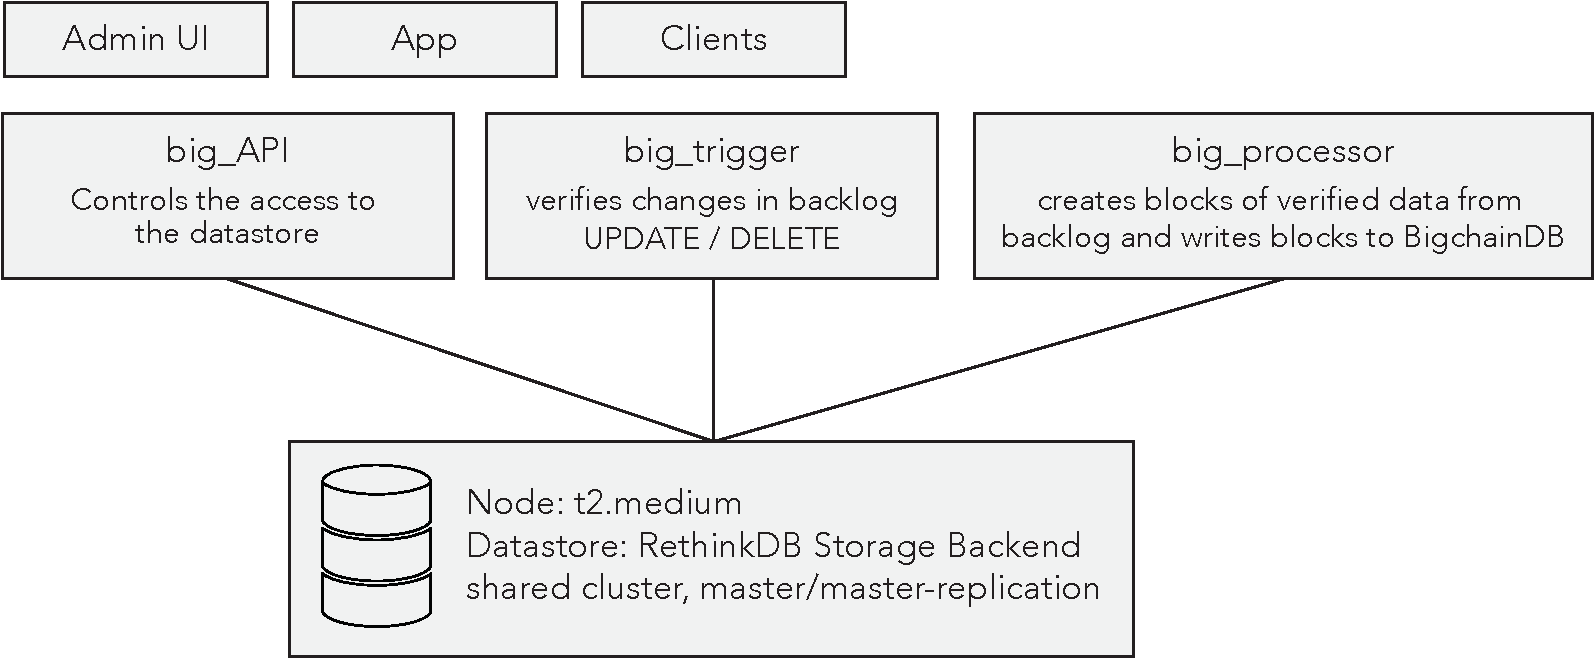
\includegraphics[width=\textwidth]{figure_9.pdf}
  \caption{BigchainDB datastore architecture.}
  \label{fig:bigchaindb_datastore_architecture}
\end{figure}

\subsection{BigchainDB Capacity}
Each t2.medium provides $48$ TB of storage, so the total capacity of $N$ nodes is $N$ times $48$ TB; with $32$ nodes, the total capacity is $1536$ TB, i.e. more than a Petabyte.
For quick reference, Figure \ref{fig:bigchain_capacity_vs_nodes} shows how total capacity depends on the number of nodes. 

\begin{figure}[!ht]
  \centering
  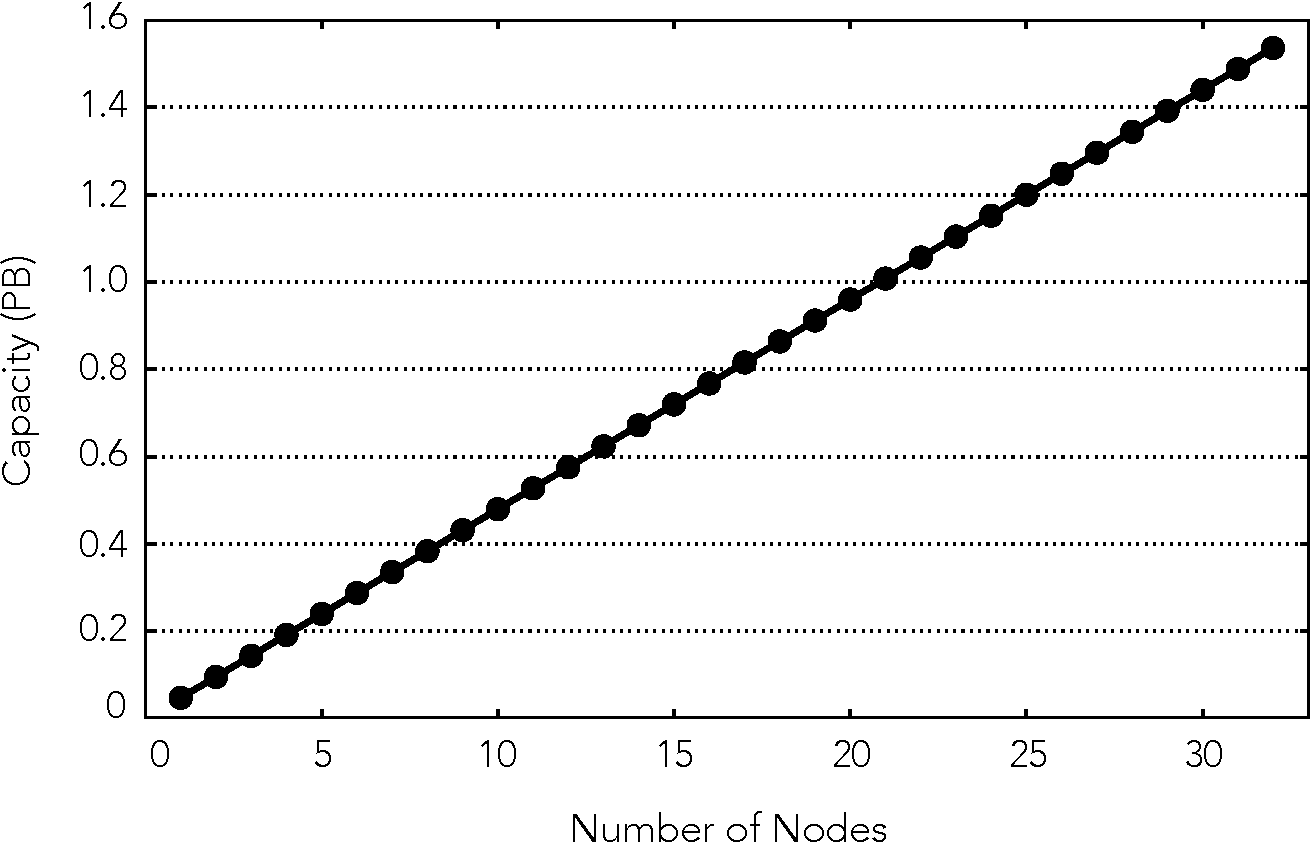
\includegraphics[width=0.8\textwidth]{figure_10.pdf}
  \caption{BigchainDB Capacity versus Number of Nodes. Each node adds another $48$ TB to the total storage capacity.}
  \label{fig:bigchain_capacity_vs_nodes}
\end{figure}

\subsection{Cryptography}

This section describes choices of cryptographic algorithms. 

\subsubsection{Hashes}

We hash using the SHA3-256 algorithm. We store the hex encoded hash in the BigchainDB. Here is a python implementation example, using pysha3\footnote{\url{https://bitbucket.org/tiran/pykeccak}}.

\begin{minipage}{\linewidth}
  \begin{lstlisting}[style=python]
  import hashlib 
  # monkey patch hashlib with sha3 functions 
  import sha3 
  data = "message" 
  tx_hash = hashlib.sha3_256(data).hexdigest()\end{lstlisting}
\end{minipage}

\subsubsection{Keys}
For signing and verifying signatures we are using the Elliptic Curve Digital Signature Algorithm (ECDSA) with $256$bit keys and the secp256k1 curve parameters, the same as used by Bitcoin and Ethereum.

The public-key or verification key are converted to string and hex encoded before storing them to BigchainDB.

\medskip
\noindent Here is a python implementation example, using \mbox{python-ecdsa}\footnote{\url{https://github.com/warner/python-ecdsa}}:

\begin{minipage}{\linewidth}
  \begin{lstlisting}[style=python]
  import binascii
  from ecdsa import SigningKey 
  # generate signing key in hex encoded form 
  sk = SigningKey.generate() 
  sk_hex = binascii.hexlify(sk.to_string()) 
  # get signing key from hex 
  sk = SigningKey.from_string(binascii.unhexlify(sk_hex))\end{lstlisting}
\end{minipage}


\subsection{Serialization}
We need to clearly define how to serialize a JSON object (RFC7159) to calculate the hash. 
The serialization should produce the same byte output independently of the architecture running the software.
If there are differences in the serialization hash validations will fail although the transaction is correct.

\medskip
\noindent Here is an example:

\begin{minipage}{\linewidth}
  \begin{lstlisting}[style=python]
  >>> a = r.expr({'a': 1}).to_json().run(b.connection)
  u'{"a":1}'
  >>> b = json.dumps({'a': 1}) 
  '{"a": 1}' 
  >>> a == b 
  False\end{lstlisting}
\end{minipage}

\medskip
\noindent We should provide the serialization and deserialization so that the following is always true.
\medskip
\noindent For example: 

\begin{minipage}{\linewidth}
  \begin{lstlisting}[style=python]
  >>> deserialize(serialize(data)) == data 
  True\end{lstlisting}
\end{minipage}


\subsubsection{Standard serialization for BigchainDB}
We are currently using the python JSON module, because it complies with the RFC.
We can specify the encoding, separators used and enforce it to order by the keys to make sure that we obtain maximum interoperability. 

\begin{minipage}{\linewidth}
  \begin{lstlisting}[style=python]
  import json 
  json.dumps(data, skipkeys=False, ensure_ascii=False, encoding="utf-8", separators=(',', ':'), sort_keys=True)\end{lstlisting}
\end{minipage}

\noindent The parameters mean: 
\begin{itemize}
 \item $\mathtt{skipkeys}$: With skipkeys $\mathtt{False}$ if the provided keys are not a string the serialization will fail. This way we enforce all keys to be strings
 \item $\mathtt{ensure\_ascii}$: The RFC recommends utf-8 for maximum interoperability. By setting $\mathtt{ensure\_ascii}$ to $\mathtt{False}$ we allow unicode characters and force the encoding to $\mathtt{utf-8}$. 
 \item $\mathtt{separators}$: We need to define a standard separator to use in the serialization. We did not do this different implementations could use different separators for serialization resulting in a still valid transaction but with a different hash e. g. an extra whitespace introduced in the serialization would still create a valid json object but the hash would be different
\end{itemize}

\subsubsection{Example}
Every time we need to perform some operation on the data like calculating the hash or signing/verifying the transaction, we need to use the previous criteria to serialize the data and then use the byte representation of the serialized data (if we treat the data as bytes we eliminate possible encoding errors e.g. unicode characters):

\begin{minipage}{\linewidth}
  \begin{lstlisting}[style=python]
  # calculate the hash of a transaction 
  # the transaction is a dictionary 
  tx_serialized = bytes(serialize(tx)) 
  tx_hash = hashlib.sha3_256(tx_serialized).hexdigest() 
  # signing a transaction 
  tx_serialized = bytes(serialize(tx)) 
  signature = sk.sign(tx_serialized) 
  # verify signature 
  tx_serialized = bytes(serialize(tx)) 
  vk.verify(signature, tx_serialized)\end{lstlisting}
\end{minipage}

\section{BigchainDB Transaction Latency}\label{sec:latency}

A key question is how long it takes for a transaction to get “etched in stone” (i.e. into a block that is \textsf{\textit{decided\_valid}}). 
To begin answering that question, we can trace the life of a transaction $\mathbf{t}$, from the time a client sends it to the time the client gets a confirmation that $\mathbf{t}$ is in a \textsf{\textit{decided\_valid}} block. 
Figure \ref{fig:bigchaindb_tx_life_1} and Figure \ref{fig:bigchaindb_tx_life_2} illustrate the life of a transaction.

\begin{figure}[!ht]
  \centering
  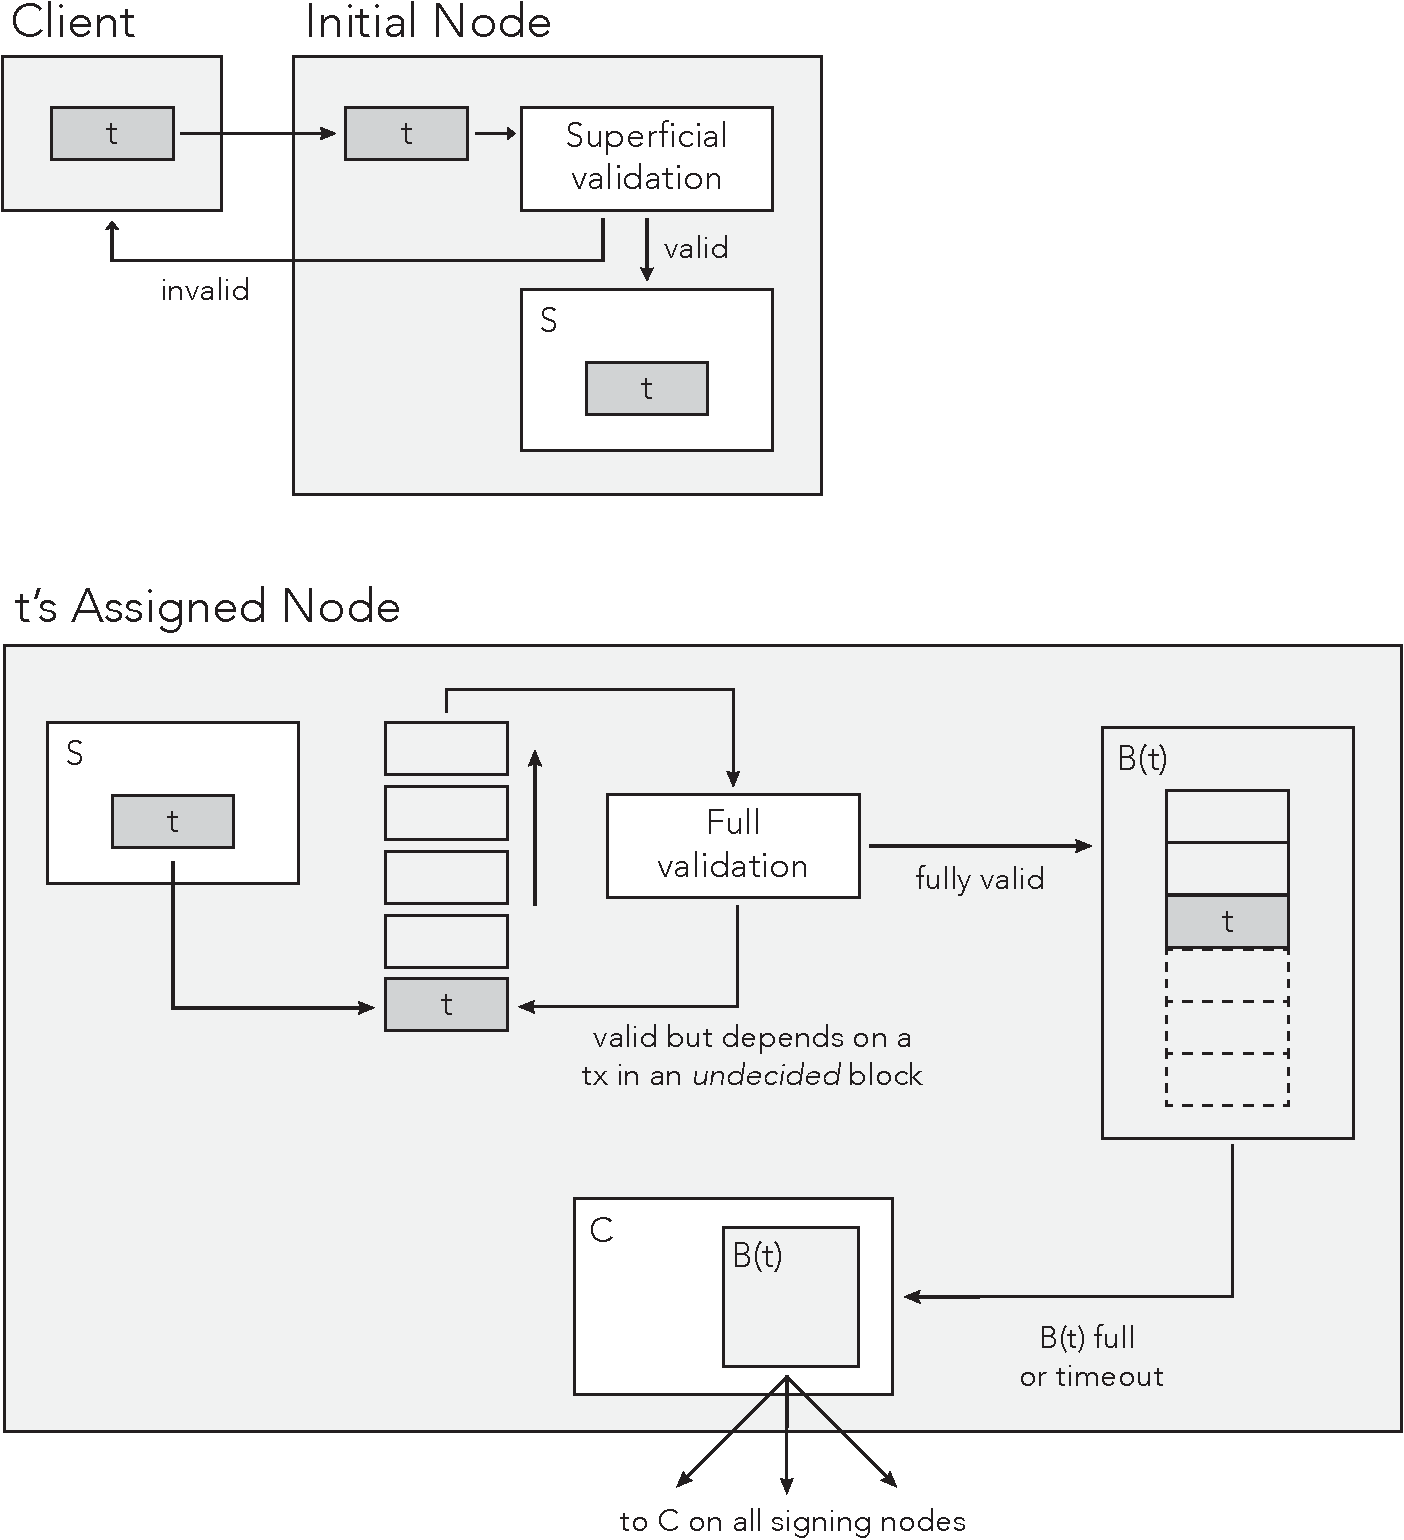
\includegraphics[width=0.8\textwidth]{figure_11.pdf}
  \caption{Life of a Transaction, Part 1/2}
  \label{fig:bigchaindb_tx_life_1}
\end{figure}

\begin{figure}[!ht]
  \centering
  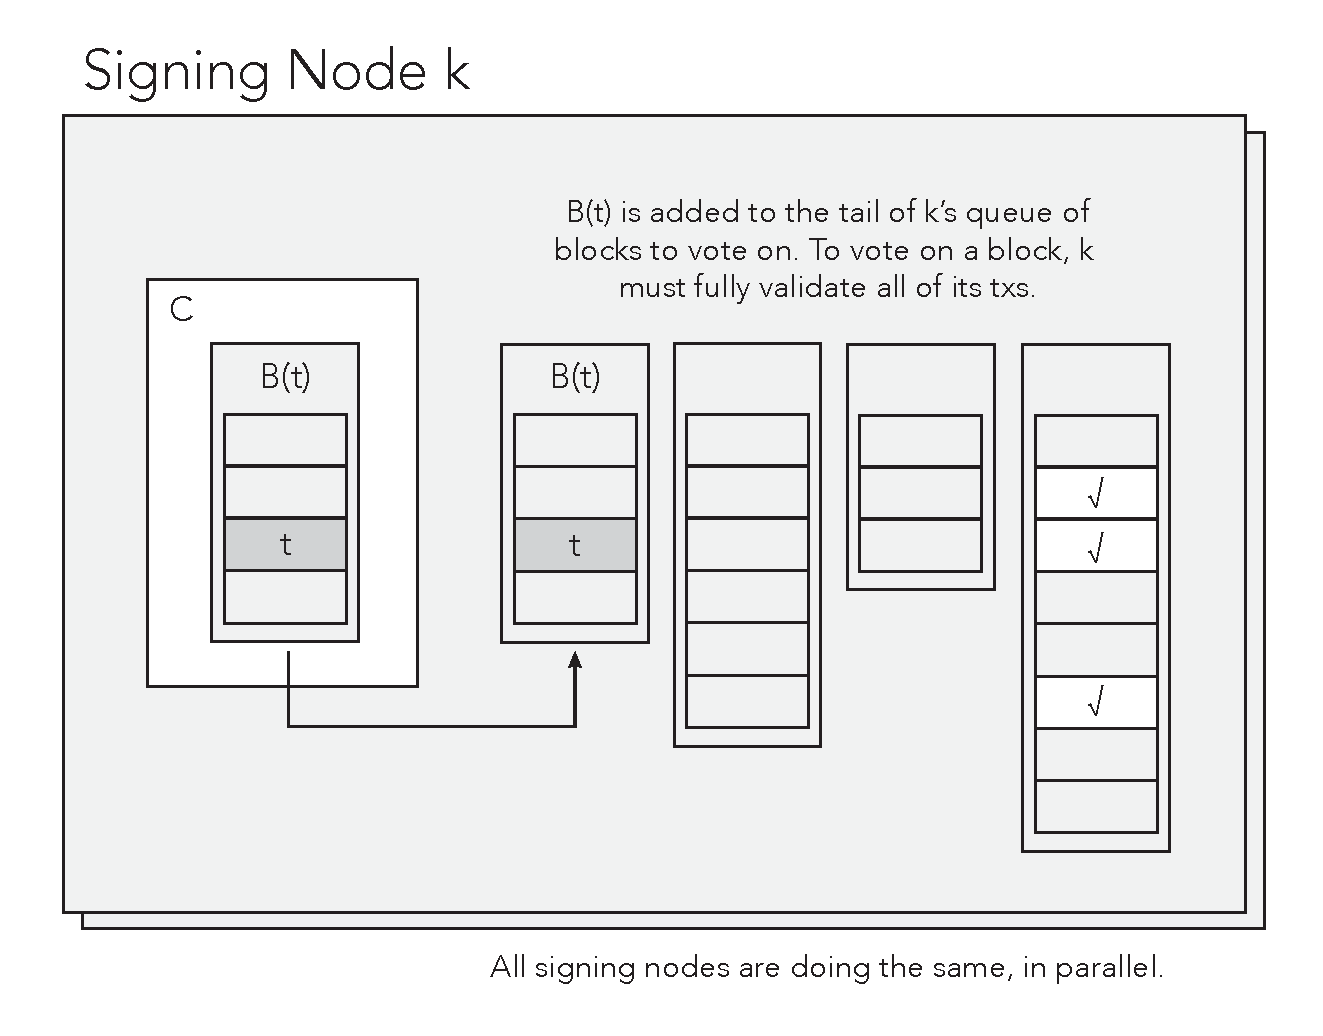
\includegraphics[width=0.6\textwidth]{figure_12_fixed.pdf}
  \caption{Life of a Transaction, Part 2/2}
  \label{fig:bigchaindb_tx_life_2}
\end{figure}

The time interval required for each step will vary. 
It can depend on how busy a node is, how busy the cluster is, network latency, and other factors. 
Nevertheless, we can still identify each step in the life of a transaction, to determine the main sources of latency.

Generally speaking, the client will send their transaction $\mathbf{t}$ over the Internet to a BigchainDB node. 
The transmission time $t_{\mathtt{in}}$ depends on how far the client is from the BigchainDB node, but it will typically range from tens to hundreds of milliseconds (ms). 
Once $\mathbf{t}$ is in a \textsf{\textit{decided\_valid}} block, a BigchainDB node can send a success notification to the client. 
The transmission time $t_{\mathtt{out}}$ will be approximately the same as $t_{\mathtt{in}}$. 
Figure \ref{fig:bigchaindb_tx_latency} illustrates $t_{\mathtt{in}}$ and $t_{\mathtt{out}}$.

We can write the total latency as:
\begin{equation}
  t_\mathtt{total} = t_{\mathtt{in}} + t_{\mathtt{internal}} + t_{\mathtt{out}}
\end{equation}

where $t_{\mathtt{internal}}$ is internal latency: the latency contributed by the Bigchain DB cluster itself. 
$t_{\mathtt{in}}$ and $t_{\mathtt{out}}$ depend on the client, but $t_{\mathtt{internal}}$ will be independent of the client (as a first approximation). 
The remainder of this section is focused on developing an estimate for $t_{\mathtt{internal}}$.

\begin{figure}[!ht]
  \centering
  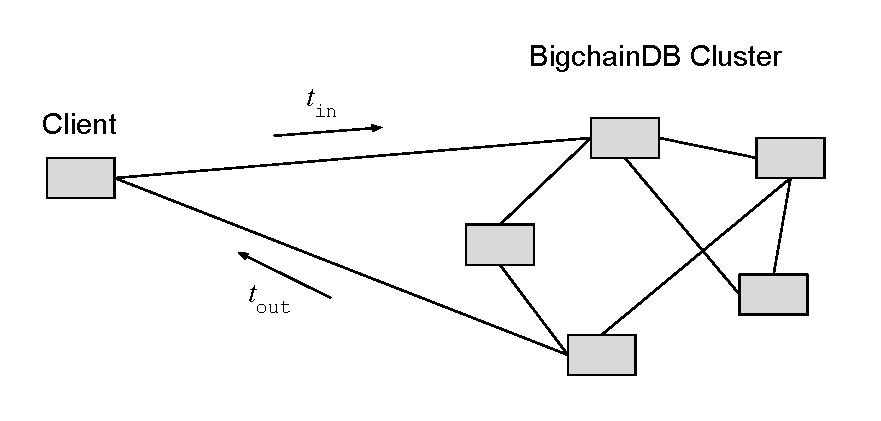
\includegraphics[width=0.7\textwidth]{figure_13.pdf}
  \caption{Transmission latencies between the client and the BigchainDB cluster.}
  \label{fig:bigchaindb_tx_latency}
\end{figure}

Let’s start with some notation.
There are many sources of latency within the BigchainDB cluster, but a key one is the time it takes information to travel from one node to another node. 
Let’s call the typical one-hop node-to-node latency $t_{\mathtt{hop}}$. The duration of $t_{\mathtt{hop}}$ depends a lot on how the nodes are distributed. 
If the nodes are all in one data center, then $t_{\mathtt{hop}}$ might be less than 1~ms. If the nodes are distributed globally, then $t_{\mathtt{hop}}$ might be $150$~ms.

Another key source of latency is query latency $t_{\mathtt{q}}$. 
If a node queries the underlying (distributed) database, it might happen that the node itself already has all the information it needs to determine the result. 
That is probably unusual, so we neglect that possibility. More typically, the required information is on one or more other nodes. 
Getting that information requires at least two internal network hops: one to send the query out, and one to get information back. 
For that case, we can write:
\begin{equation}\label{eq:time_query}
t_\mathtt{q} \ge (2 \cdot t_\mathtt{hop}) + t_\mathtt{qp}
\end{equation}
where $t_\mathtt{qp}$ is the query processing time. 

If all nodes in the cluster are in one data center, then $t_\mathtt{hop}$ and $t_\mathtt{qp}$ might be similar in duration, so we may not be able to neglect $t_\mathtt{qp}$ relative to $t_\mathtt{hop}$.

Let’s return to figuring out a back-of-the-envelope estimate for $t_\mathtt{internal}$.
In general, it could be quite large, because a transaction might bounce back and forth between the backlog $\mathbf{S}$ and the bigchain $\mathbf{C}$ before it finally ends up in a \textsf{\textit{decided\_verified}} block.
What we \textit{can} do is determine an approximate \textit{minimum} $t_\mathtt{internal}$ (i.e. a lower bound).

When $\mathbf{t}$ arrives at a BigchainDB node, the node does a superficial validation of $\mathbf{t}$ (i.e. not checking if it depends on a transaction in an undecided block). 
That requires at least one query (e.g. to check if $\mathbf{t}$ does a double-spend), so the time required is at least $t_\mathtt{q}$. 
(If $\mathbf{t}$ is invalid, then the client can be notified and that’s the end of the story for $\mathbf{t}$.)

If $\mathbf{t}$ is valid, then the BigchainDB node assigns $\mathbf{t}$ to a randomly-choosen node. 
It then writes $\mathbf{t}$ to the backlog ($\mathbf{S}$). 
The underlying distributed database will notify all the other nodes about the change to $\mathbf{S}$ (i.e. that there is a new transaction), along with the contents of $\mathbf{t}$. 
It takes at least $t_\mathtt{hop}$ time for $\mathbf{t}$ to propagate over the internal BigchainDB network.

$\mathbf{t}$ then enters the tail of a queue on the assigned node, where it waits for the assigned node to check it for validity (including whether $\mathbf{t}$ depends on a transaction in an \textsf{\textit{undecided}} block). 
In general, there may be several transactions ahead of $\mathbf{t}$ in that queue. 
The assigned node must check each of those transactions first; each check requires at least one query, so at least $t_\mathtt{q}$ time is needed to check each transaction ahead of $\mathbf{t}$. 
In the best case, there are no transactions ahead of $\mathbf{t}$ in the assigned node’s queue, so the waiting time is zero.

Once $\mathbf{t}$ gets its turn at being considered, the assigned node must check to see if $\mathbf{t}$ is valid (including whether $\mathbf{t}$ depends on a transaction in an \textsf{\textit{undecided}} block). 
That takes at least $t_\mathtt{q}$ time. 
If $\mathbf{t}$ \textit{does} depend on a transaction in an \textsf{\textit{undecided}} block, then it must go back to waiting for consideration for inclusion in a block (i.e. back to the tail of the assigned node’s queue).

Suppose $\mathbf{t}$ is okayed for inclusion in a block. 
Let’s call that block $\mathbf{B}(\mathbf{t})$. 
$\mathbf{t}$ must wait for $\mathbf{B}(\mathbf{t})$ to accumulate $1000$ transactions (or whatever value the BigchainDB operator sets), or for a timeout to occur (e.g. five seconds since the last transaction was added to the block). 
The timeout is to ensure that a block doesn’t wait forever for new transactions. 
When there are lots of new transactions coming in, the time $\mathbf{t}$ spends waiting for $\mathbf{B}(\mathbf{t})$ to fill up will typically be negligible compared to $t_\mathtt{hop}$, so we can ignore it.

The assigned node then writes $\mathbf{B}(\mathbf{t})$ to $\mathbf{C}$. It takes time for $\mathbf{B}(\mathbf{t})$ to propagate to all other nodes in the cluster: at least $t_\mathtt{hop}$.

Each signing node will be notified about the new block $\mathbf{B}(\mathbf{t})$, including its contents. Signing node $\mathbf{k}$ will add the newly-arrived block to the tail of its queue of blocks to vote on. 
$\mathbf{k}$’s local copy of $\mathbf{B}(\mathbf{t})$ will wait for $\mathbf{k}$ to vote on all other blocks ahead of $\mathbf{B}(\mathbf{t})$ in $\mathbf{k}$’s queue. 
In the best case, there are no nodes ahead of $\mathbf{B}(\mathbf{t})$ in $\mathbf{k}$’s queue, so the waiting time is zero.

How long does it take for a node to vote on one block? 
If there are $1000$ transactions in the block, then the node may have to check the validity of all $1000$ transactions. 
(It doesn’t always have to check all the transactions: if it finds an invalid one, it can stop before checking any more.) 
Once the validity checks are done, the node must compose a vote (data structure) and calculate its digital signature, but the time to do that is negligible compared to the time needed to check validity.

The node doesn’t have to check the validity of each transaction one at a time. 
It can check many transactions in parallel at the same time, depending on how many processes are available to do validity-checking. 
In principle, there may be sufficient processors available to check all transactions for validity in parallel at once. 
Therefore, in the best case, the time to vote on one block will be approximately the same as the time to check one transaction for validity: $t_\mathtt{q}$.

Once $\mathbf{B}(\mathbf{t})$ gets to the head of $\mathbf{k}$’s queue, $\mathbf{B}(\mathbf{t})$ might already be decided, but $\mathbf{k}$ votes on it regardless (i.e. $\mathbf{k}$ doesn’t spend time checking if $\mathbf{B}(\mathbf{t})$ is already decided). 
As explained above, voting on $\mathbf{B}(\mathbf{t})$ takes at least $t_\mathtt{q}$ time.

Once $\mathbf{B}(\mathbf{t})$ has gotten votes from a majority of the signing nodes, it becomes either \textsf{\textit{decided\_valid}} or \textsf{\textit{decided\_invalid}}. 
(The list of nodes which can vote on $\mathbf{B}(\mathbf{t})$ is set when $\mathbf{B}(\mathbf{t})$ is created, and doesn’t change if nodes are added or removed from the cluster.) 
The deciding vote takes time $t_\mathtt{hop}$ to propagate to all the other nodes in the cluster.

If $\mathbf{B}(\mathbf{t})$ is \textsf{\textit{decided\_invalid}} then the transactions inside $\mathbf{B}(\mathbf{t})$ (including $\mathbf{t}$) get sent back to $\mathbf{S}$ for reconsideration in a future block.

If $\mathbf{B}(\mathbf{t})$ is \textsf{\textit{decided\_valid}}, then $\mathbf{t}$ is “etched in stone” and a success notification message can be sent to the client.

We can now estimate a minumum $t_\mathtt{internal}$ by adding up all the times outlined in the precedinging paragraphs:

\begin{equation}
 t_\mathtt{internal} \ge 3 \cdot t_\mathtt{q} + 3 \cdot t_\mathtt{hop}
\end{equation}

Then, using Eq.~\eqref{eq:time_query}:

\begin{equation}
 t_\mathtt{internal} \ge 9 \cdot t_\mathtt{hop} + 3 \cdot t_\mathtt{qp} 
\end{equation}

If the cluster nodes are widely-distributed, then $t_\mathtt{hop}$ is much larger than $t_\mathtt{qp}$ and:

\begin{equation}
 t_\mathtt{internal} \ge 9 \cdot t_\mathtt{hop}
\end{equation}

As a rule of thumb for widely-distributed clusters, \textit{the minimum internal latency is about an order of magnitude larger than the one-hop node-to-node latency}. 
(Remember that $t_\mathtt{internal}$ ignores client-to-BigchainDB network latency.)

There are a few general cases, depending on how the BigchainDB nodes are distributed. Table \ref{tab:latency_comparison} summarizes.

\begin{savenotes}
\begin{table}[ht!]
  \caption{Latency based on geographic distribution of the cluster}
  \footnotesize
  \makebox[\textwidth][c]{
  \setlength\extrarowheight{3pt}
  \begin{tabular}{ | m{\dimexpr 0.3\linewidth-2\tabcolsep} |
	  M{\dimexpr 0.35\linewidth-2\tabcolsep} |
	  M{\dimexpr 0.35\linewidth-2\tabcolsep} |} \Xhline{4\arrayrulewidth}\rowcolor{black}
    \color{white}How nodes are distributed    &  \color{white} One-hop node-to-node latency in the cluster ($t_\mathtt{hop}$) & \color{white} Minimum internal transaction latency in the cluster (minimum~$t_\mathtt{internal}$) \\\Xhline{4\arrayrulewidth}
    In one data center           & $\approx 0.25$ ms & $\approx 2.25\ \mathrm{ms} + 3 \cdot t_\mathtt{qp}$ \\\hline
    In one region (e.g. America) & $\approx 70$ ms   & $\approx 630$ ms \\\hline
    Spread globally              & $\approx 150$ ms  & $\approx 1350$ ms \\
  \Xhline{4\arrayrulewidth}
  \end{tabular}
  }
  \label{tab:latency_comparison}
\end{table}
\end{savenotes}

There are a couple of caveats to keep in mind when reading Table~\ref{tab:latency_comparison}: 1)~The minimum internal latency estimates in Table \ref{tab:latency_comparison} are order-of-magnitude approximations. They should only be interpreted as \emph{guidelines} for what to expect. 2)~In a data center, the query latency $t_{\mathtt{qp}}$ may be similar in magnitude to $t_\mathtt{hop}$, so to get a better estimate of the minimum internal latency, one needs an estimate of $t_{\mathtt{qp}}$.

\section{Private vs. Public BigchainDB, and Authentication}\label{sec:permissioning}

\subsection{Introduction}
The way that BigchainDB is designed, permissioning sits at a layer above the core of the design. 
However, we have already seen many questions about “private vs. public” versions of BigchainDB, privacy, and authentication. 
In our view, a rich permissioning framework is the technology foundation. 
This section explores permissions, roles, private BigchainDBs, and privacy. 
It then has an extended section on a public BigchainDB, which we believe is tremendously important. 
It finally discusses authentication and the role of certificate-granting authorities.

\subsection{Permissions, Identities, and Roles}
Permissions are rules about what a user can do with a piece of data. 
Permissions are used in all kinds of computing environments, from shared file systems like Dropbox and Google Drive, to local file systems in Windows, iOS, and Linux, to distributed DBs. 
We should expect blockchain DBs to have rich permissioning systems.

Permissioning ideas from these other systems can inform our design. 
In Unix, each file or directory has three identity roles (owning user, owning group, others) and three types of permissions for each role (read, write, execute), for a total of nine permission values. 
For example, the permission values ``\texttt{rwxr--r---}'' means that the owning user can read, write, and execute (\texttt{rwx}); the owning group can read but not write or execute (\texttt{r--}), and others have no permissions (\texttt{---}).

A BigchainDB database instance is characterized by which identities have which permissions. 
Table \ref{tab:permissioning_enterprise} and Table \ref{tab:permissioning_public} gives examples of permissions on a private and public BigchainDB, respectively. 
This is loosely comparable to a corporation’s internal intranet and the public Internet. 
We will elaborate on these shortly.

\begin{savenotes}
\begin{table}[ht!]
  \caption{Example Permissioning / Roles in an Enterprise BigchainDB Instance}
  \footnotesize
  \makebox[\textwidth][c]{
  \centering
  \setlength\extrarowheight{3pt}
  \begin{tabular}{ | m{\dimexpr 0.2\linewidth-2\tabcolsep} |
	  M{\dimexpr 0.12\linewidth-2\tabcolsep} |
	  M{\dimexpr 0.1\linewidth-2\tabcolsep} |
	  M{\dimexpr 0.1\linewidth-2\tabcolsep} |
	  M{\dimexpr 0.1\linewidth-2\tabcolsep} |
	  M{\dimexpr 0.1\linewidth-2\tabcolsep} |
	  M{\dimexpr 0.1\linewidth-2\tabcolsep} |
	  M{\dimexpr 0.16\linewidth-2\tabcolsep} |
	  M{\dimexpr 0.1\linewidth-2\tabcolsep} |
	  M{\dimexpr 0.12\linewidth-2\tabcolsep} | } \Xhline{4\arrayrulewidth}\rowcolor{black}\color{white}
  Action    & \color{white} Requires vote & \color{white} Voting Node & \color{white} Sys Admin & \color{white} Issuer & \color{white} Trader & \color{white}Broker & \color{white} Authenticator & \color{white} Auditor & \color{white} Core vs Overlay \\\Xhline{4\arrayrulewidth}
  Vote on Admin \& Asset Actions & & Y & & & & & & & \textbf{Core} \\\Xhline{2\arrayrulewidth}\rowcolor{backcolour}
  \multicolumn{10}{|c|}{Admin actions}\\\Xhline{2\arrayrulewidth}
  Update Role or Permissions & Y & Y & Y & & & & & & \textbf{Core} \\\hline
  Add/Remove Voting Node & Y & Y & Y\footnote{\label{note:permissioning_sysadmin}Action is permitted only during the network initiatization process. Once a network is live, the sys admin can no longer act unilaterally.} & & & & & & \textbf{Core} \\\hline
  Update software & Y & Y & Y & & & & & & \textbf{Core} \\\Xhline{2\arrayrulewidth}\rowcolor{backcolour}
  \multicolumn{10}{|c|}{Asset actions}\\\Xhline{2\arrayrulewidth}
  Issue Asset                        & Y & & & Y &   &   &   & & \textbf{Core} \\\hline
  Transfer Asset                     & Y & & & O & O & P &   & & \textbf{Core} \\\hline
  Receive Asset                      & Y & & & Y & Y &   &   & & \textbf{Core} \\\hline
  Grant Read Access on Asset         & Y & & & O & O & P & P & & \textbf{Core} \\\hline
  Consign Asset                      & Y & & & O & O &   &   & & \textbf{Overlay} \\\hline
  Receive Asset Consignment          & Y & & & Y & Y & Y &   & & \textbf{Overlay} \\\hline
  Add Asset Information              & Y & & & O & O & P &   & & \textbf{Overlay} \\\hline
  Add Authentication Information     & Y & & & O & O &   & P & & \textbf{Overlay} \\\hline
  Create Certificate of Authenticity & N & & & O & O & P &   & & \textbf{Overlay} \\\Xhline{2\arrayrulewidth}\rowcolor{backcolour}
  \multicolumn{10}{|c|}{Read actions}\\\Xhline{2\arrayrulewidth}
  Read Asset Information             & N & Y & Y & O & Y & P & P & P & \textbf{Overlay} \\\hline
  Read Certificate of Authenticity   & N & Y & Y & O & Y & P & P & P & \textbf{Overlay} \\
  \Xhline{4\arrayrulewidth}
  \end{tabular}
  }
  \label{tab:permissioning_enterprise}
\end{table}
\end{savenotes}

An \textbf{identity}, which signifies the holder of a unique private key, can be granted a \textbf{permission} for each transaction type. 
Permissions, as reflected on the tables, can be as follows: “\textbf{Y}” means the identity can perform a transaction; “\textbf{O}” means the identity can perform a transaction if the identity is the owner of the asset, which is indicated by holding the private key to that asset; and “\textbf{P}” means can perform a transaction, after the owner of the asset has given permission to the identity. 
Most transactions need to be voted as approved or not approved by voting nodes, with the exception of read operations.

A role is a group of individual permissions. 
Roles facilitate permission assignment and help clarify the rights given to users in their identity and with their permissions. 
Roles can be custom-created depending on the context. 
An identity may hold multiple roles, where the identity’s permissions are the sum of the identity’s role permissions and any other permissions that have been granted to it.

The core BigchainDB protocol includes as few actions or transaction types as possible, in order to maximize backwards-compatibility and minimize complexity. 
Overlay protocols can add new features, such as SPOOL \cite{dejonghe_spool} for unique asset ownership, which adds actions like consignment and authentication to property transactions. 
Table \ref{tab:permissioning_enterprise} and Table \ref{tab:permissioning_public} each have core protocol actions, as well as some overlay protocol actions from SPOOL.

\subsection{Private BigchainDBs}
A private BigchainDB could be set up amongst a group of interested parties to facilitate or verify transactions between them in a wide variety of contexts, such as exchanging of securities, improving supply chain transparency, or managing the disbursement of royalties. 
For instance, the music industry could choose to form a trust network including record labels, musicians, collecting societies, record stores, streaming services, and support providers such as lawyers and communications agencies. 
A consortium of parties operating a private BigchainDB comprise an “enterprise trust network” (ETN).

Table \ref{tab:permissioning_enterprise} illustrates permissioning of a sample private BigchainDB instance for use in an ETN.

The first column shows actions allowed; the second column shows whether the action needs voting; columns 3-9 are roles; and the final column indicates whether the action is part of the core BigchainDB protocol.

An identity holding the “Voting Node” role (column 3) can vote on asset actions. No other role is able to do so.

Voting Nodes can update permissions for any other identity (row 2). 
Changing permissions requires voting consensus from other nodes. 
This is how new identities entering the system are assigned permissions or roles, and also how Voting Nodes are added or removed.

A Voting Node may propose an update to the Voting Node software (row 4).
Voting Nodes will only update once they reach consensus.
Voting Nodes also must be able to read an asset (rows 14-15) in order to be able to vote.

Like a Voting Node, an identity with “Sys Admin” role can propose to update permissions or update voting node software. 
This role is helpful because voting nodes may not be up-to-date technically when the Sys Admin is. 
Crucially, the Sys Admin cannot unilaterally update the software; rather, it can only propose software and ensure that the voting nodes hit consensus about updating. 
The Sys Admin must also be able to read an asset (rows 14-15), in order to debug issues that may arise with the software.

The main job of the “Issuer” role is to issue assets (row 5).
But it can also do everything that a Trader role can do.

The “Trader” role conducts trades of assets, has others conduct trades on its behalf, and lines up reading and authentication of assets.
It can transfer ownership to an identity, though only if it is the owner of the asset as indicated by the “O” (row 6); or be on the receiving end of an asset transfer (row 7).
Similarly, if it is the owner then it can consign an asset to have another identity transact with the asset on its behalf (row 9); or be on the receiving end as consignee (row 10). By default, read permissions are off, but a Trader can allow others to read the asset info (row 10 grants permission; row 15 read). The Trader can also add arbitrary data or files to an asset (row 11).

A “Broker / Consignee” role (column 7) gets a subset of the Trader’s permissions - only what is needed to be able to sell the work on the owner’s behalf.

We describe the “Authenticator” role (column 8) further in section \ref{subsec:permissioning_authentication}.

For simplicity of presentation, some details have been omitted compared to the actual implementation.
For example, usually a Consignee has to accept a consignment request.

\subsection{Privacy}

\noindent \textbf{Q}: Bank A doesn’t want Bank B to see their transactions.
But if they’re both voting nodes, can Bank B see Bank A’s transactions?

\noindent \textbf{A}: This is not really related to BigchainDB; it doesn’t care about the content of the transaction.
For the transaction to be valid, it just needs to have a current unspent input and a correct signature.

\medskip
\noindent \textbf{Q}: But if every voting node knows the identity of the nodes in a transaction, and can see the amount transacted in order to validate the transaction, than isn’t that a loss of privacy?

\noindent \textbf{A}: The nodes in a transaction are just public keys.
The way that the mapping between a public key and an identity is done should be taken care of by Bank A and Bank B.
If they want to hide the amount that is being transacted, they can do that; BigchainDB doesn't care.

Let’s say that Bank A creates an input “A” and gives it to “PUBKA”, and inside the data field it says that this is an input for “B”, and “B” is just a serial number.
BigchainDB makes sure that input “A” can only be spent once and that only “PUBKA” can spend it.
There are no amounts involved.

\subsection{A Public BigchainDB}\label{subsec:permissioning_public}
\subsubsection{Introduction}
A BigchainDB can be configured to be more public, with permissioning such that anyone can issue assets, trade assets, read assets, and authenticate. 
We are taking steps towards a first public BigchainDB\footnote{We envision that ultimately there will be many public BigchainDBs. More than one is not a big problem, as there is no native token built into the DB. Universal resource indicators (URIs) will make them easy to distinguish.}.

\subsubsection{Motivations}

Decentralization technology has potential to enable a new phase for the Internet that is open and democratic but also easy to use and trust \cite{swan2015blockchain}\cite{andreesen2014bitcoin}\cite{monegro2014blockchain_stack}.
It is intrinsically democratic, or at the very least disintermediating.
It is also trustworthy: cryptography enables the conduct of secure and reliable transactions with strangers without needing to trust them, and without needing a brand as proxy.

The discourse is around benefits in both the public and private sector.
In the public sector, the most obvious benefit is in the future shape of the Internet and especially the World Wide Web \cite{berners1989information_mgmnt}.
These technologies have fundamentally reshaped society over the past two decades. The 90s Web started out open, free-spirited, and democratic. 
In the past 15 years, power has consolidated across social media platforms and the cloud.
People around the world have come to trust and rely on these services, which offer a reliability and ease of use that did not exist in the early Internet. 
However, these services are massively centralized, resulting in both strict control by the central bodies and vulnerability to hacking by criminals and nation-states.

Decentralization promises a large positive impact on society. 
An antidote to these centralized services and concentration of power is to re-imagine and re-create our Internet via decentralized networks, with the goal of giving people control over their data and assets and redistributing power across the network.

\subsubsection{Public BigchainDB Roles}

\begin{table}[ht!]
  \caption{Example Permissioning / Roles in an Public BigchainDB}
  \footnotesize
  \makebox[\textwidth][c]{
  \centering
  \setlength\extrarowheight{3pt}
  \begin{tabular}{ | m{\dimexpr 0.3\linewidth-2\tabcolsep} |
	  M{\dimexpr 0.12\linewidth-2\tabcolsep} |
	  M{\dimexpr 0.1\linewidth-2\tabcolsep} |
	  M{\dimexpr 0.1\linewidth-2\tabcolsep} |
	  M{\dimexpr 0.1\linewidth-2\tabcolsep} |
	  M{\dimexpr 0.1\linewidth-2\tabcolsep} |
	  M{\dimexpr 0.17\linewidth-2\tabcolsep} |} \Xhline{4\arrayrulewidth}\rowcolor{black}\color{white}
  Action    & \color{white} Requires vote & \color{white} Voting Node & \color{white} Sys Admin & \color{white} Issuer & \color{white} User & \color{white} Authenticator \\\Xhline{4\arrayrulewidth}
  Vote on Admin \& Asset Actions & & Y & & & & \textbf{Core} \\\Xhline{2\arrayrulewidth}\rowcolor{backcolour}
  \multicolumn{7}{|c|}{Admin actions}\\\Xhline{2\arrayrulewidth}
  Update Role or Permissions & Y & Y & Y & & & \textbf{Core} \\\hline
  Add/Remove Voting Node & Y & Y & Y\footnotemark[\getrefnumber{note:permissioning_sysadmin}] & & & \textbf{Core} \\\hline
  Update software & Y & Y & Y & & & \textbf{Core} \\\Xhline{2\arrayrulewidth}\rowcolor{backcolour}
  \multicolumn{7}{|c|}{Asset actions}\\\Xhline{2\arrayrulewidth}
  Issue Asset                        & Y & & & Y &   & \textbf{Core} \\\hline
  Transfer Asset                     & Y & & & O &   & \textbf{Core} \\\hline
  Receive Asset                      & Y & & & Y &   & \textbf{Core} \\\hline
  Grant Read Access on Asset         & Y & & & N/A & N/A & \textbf{Core} \\\hline
  Consign Asset                      & Y & & & O &   & \textbf{Overlay} \\\hline
  Receive Asset Consignment          & Y & & & Y &   & \textbf{Overlay} \\\hline
  Add Asset Information              & Y & & & O &   & \textbf{Overlay} \\\hline
  Add Authentication Information     & Y & & & O & P & \textbf{Overlay} \\\hline
  Create Certificate of Authenticity & N & & & O &   & \textbf{Overlay} \\\Xhline{2\arrayrulewidth}\rowcolor{backcolour}
  \multicolumn{7}{|c|}{Read actions}\\\Xhline{2\arrayrulewidth}
  Read Asset Information             & N & Y & Y & O & P & \textbf{Overlay} \\\hline
  Read Certificate of Authenticity   & N & Y & Y & O & P & \textbf{Overlay} \\
  \Xhline{4\arrayrulewidth}
  \end{tabular}
  }
  \label{tab:permissioning_public}
\end{table}

Table \ref{tab:permissioning_public} describes permissioning of a public BigchainDB instance.
Here, BigchainDB is configured such that each User (column 6) can do anything, except for sensitive roles such as voting, administration, and authentication.
Critically, Users can issue any asset (column 6, row 5) and read all assets (column 6, row 14); this is one of the defining features of an open blockchain. 

\subsubsection{Public BigchainDB Federation Caretakers}

At the core of a public BigchainDB are the “Caretakers”: organizations with an identity that has a “Voting Node” role.
An identity with that role can vote to approve or reject transactions, and can vote whether to assign the “Voting Node” role to another identity. 
(Note: an organization can have more than one identity, so a Caretaker could have two or more identities with a “Voting Node” role.)

To start, the public BigchainDB will have five identities with the Voting Node role: three held by ascribe and two held by other organizations chosen by ascribe.
That is, the public BigchainDB will start with three Caretakers: ascribe and two others.
From there, additional Caretakers will be selected and added to the federation by existing Caretakers.
Caretakers will have divergent interests to avoid collusion, but must have one thing in common: they must have the interests of the Internet at heart.
In choosing Caretakers, there will be a preference to organizations that are non-profit or building foundational technology for a decentralized Internet; and for diversity in terms of region, language, and specific mandate.

The right organizational structure will be critical to the success of a public BigchainDB.
Governance issues have plagued the Bitcoin blockchain \cite{popper2016bitcoin_crisis}.
We can take these as lessons in the design of a public BigchainDB.
We are consulting with lawyers, developers, academics, activists, and potential Caretakers to develop a strong, stable system that is transparent enough to be relied on and flexible enough to meet the needs of the network.

Ultimately, the public BigchainDB will operate entirely independently under its own legal entity.
It will choose its own Caretakers and set its own rules—but it will always work toward the long-term goal of a free, open, and decentralized Internet.

\medskip

\fbox{\begin{minipage}{\linewidth}
\centering
\medskip
We are gathering a consortium of potential public BigchainDB nodes. If you think your organization fits as one of these nodes, or have suggestions for nodes, please contact the authors.
\medskip
\end{minipage}}

\subsection{BigchainDB Authentication of Assets}\label{subsec:permissioning_authentication}

The “Authenticator” role gives a formal place for authentication and certificate-granting authorities.
Examples may include a credit rating agency, an art expert certifying the authenticity of a painting, a university issuing a degree, a governmental body issuing a permit, or a notary stamping a document.

While the BigchainDB can function completely without the Authenticator role, in a decentralized network where anyone can issue assets, it is clear that third parties will step in to provide an extra layer of trust for asset buyers.

These third parties would do all the things trusted third parties do today—act as an escrow agent, place a stamp or seal of approval, issue a certificate, or rate the quality or reputation of the asset issuer.

For authentication to be issued, a Trader enables an identity to have read and authentication permission on an asset (Table \ref{tab:permissioning_enterprise}, row 8), then the Authenticator reviews all relevant information about the asset, and issues a report as a transaction (Table \ref{tab:permissioning_enterprise}, row 12).

The owner of the asset may then create a cryptographic Certificate of Authenticity (COA), a digital document that includes all the digitally signed authentication reports from the various authenticators.
The COA is digitally signed as well, so even if printed out, tampering can be detected.
The COA can then be used by the seller as a pointer to authenticity, to show that the asset is not fraudulent.

A public BigchainDB should not be prescriptive—it should be open to new sources of authority.
The issuance of certificates does not have to be limited to traditional authorities.
BigchainDB allows flexibility in this respect, remaining open to the many possible approaches that will undoubtedly be created by users.
BigchainDB therefore limits its role to providing a mechanism for reliable gathering and aggregation of signed data.

We imagine a rich community of authorities signing assets. 
For example, point-of-creation software or hardware vendors could certify that a particular digital creation was created by their software or hardware at a given point in time. 
Individuals could leave certified reviews for movies, restaurants, consumer goods, or even reputational reviews for other individuals.
Other examples could emerge from ideas in prediction markets \cite{hanson1993consensus}, the issuance of securities, and the rating of those securities.

In a model where anyone can issue an authoritative statement about someone or something, the reputation of the Authenticator will be critically important.
How do you know whose certificates you can trust?
We anticipate the development of social media reputation systems that go beyond Facebook Friends and Likes.
BigchainDB enables the widespread implementation of new reputation systems such as the Backfeed protocol for management of distributed collaboration \cite{backfeed}, or systems drawing inspiration from fictional reputation economies described by Cory Doctorow (Whuffie) \cite{doctorow2003down}, Daniel Suarez (Levels) \cite{suarez2010freedomtm}, and others.

\section{Experimental Results}\label{sec:benchmarks}

\subsection{Goals}

BigchainDB's algorithms are designed to ``get out of the way'' of the underlying database, so we expect the main limiter on performance to be how that underlying database interacts with the physical compute resources (e.g.~write speed and I/O among nodes).
Because of that, and because BigchainDB is built on top of RethinkDB, we began with experiments to test the scalability properties of RethinkDB.

Full benchmarks on the performance of BigchainDB will appear in the near future.

\subsection{Experiments on Throughput}

Appendix~\ref{subsec:benchmarks_setup} describes the details of the experimental setups.

In one experiment, we increased the number of nodes every ten seconds, up to $32$ nodes.
We used RethinkDB's System Statistics Table to record the write throughput over time.

\begin{figure}[!ht]
  \centering
  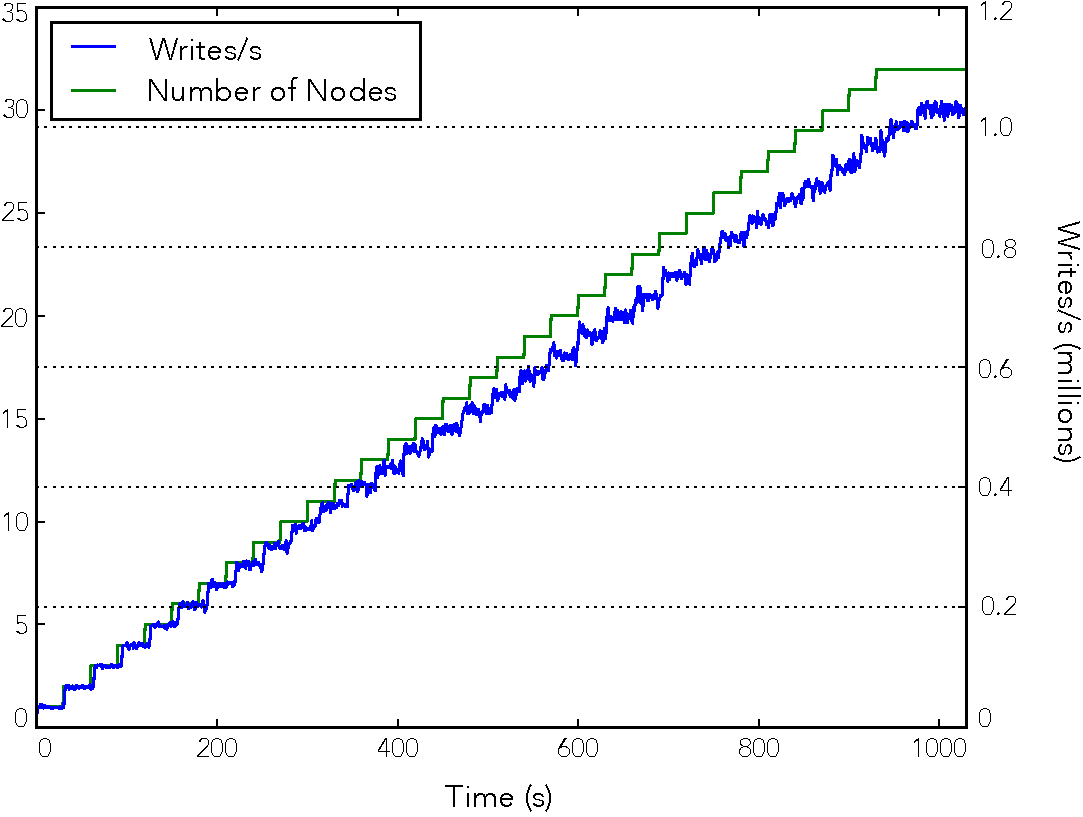
\includegraphics[width=0.7\textwidth]{figure_14.pdf}
  \caption{Time-series plot, where when we increased the number of nodes, the throughput increased proportionately.}
  \label{fig:bigchain_throughput_vs_nodes}
\end{figure}

Figure~\ref{fig:bigchain_throughput_vs_nodes} shows how write throughput increased every time a node was added.
When the number of nodes reached $32$, the write throughput was just over $1$~million transactions per second (i.e.~$1000$ blocks written per second, with $1000$ valid transactions per block).\footnote{
In Figure~\ref{fig:bigchain_throughput_vs_nodes}, the y-axis label of ``Writes/s'' should be interpreted to mean ``Effective transaction-writes per second''. The same is true of Figure~\ref{fig:bigchain_writes_vs_nodes}.}

\begin{figure}[!ht]
  \centering
  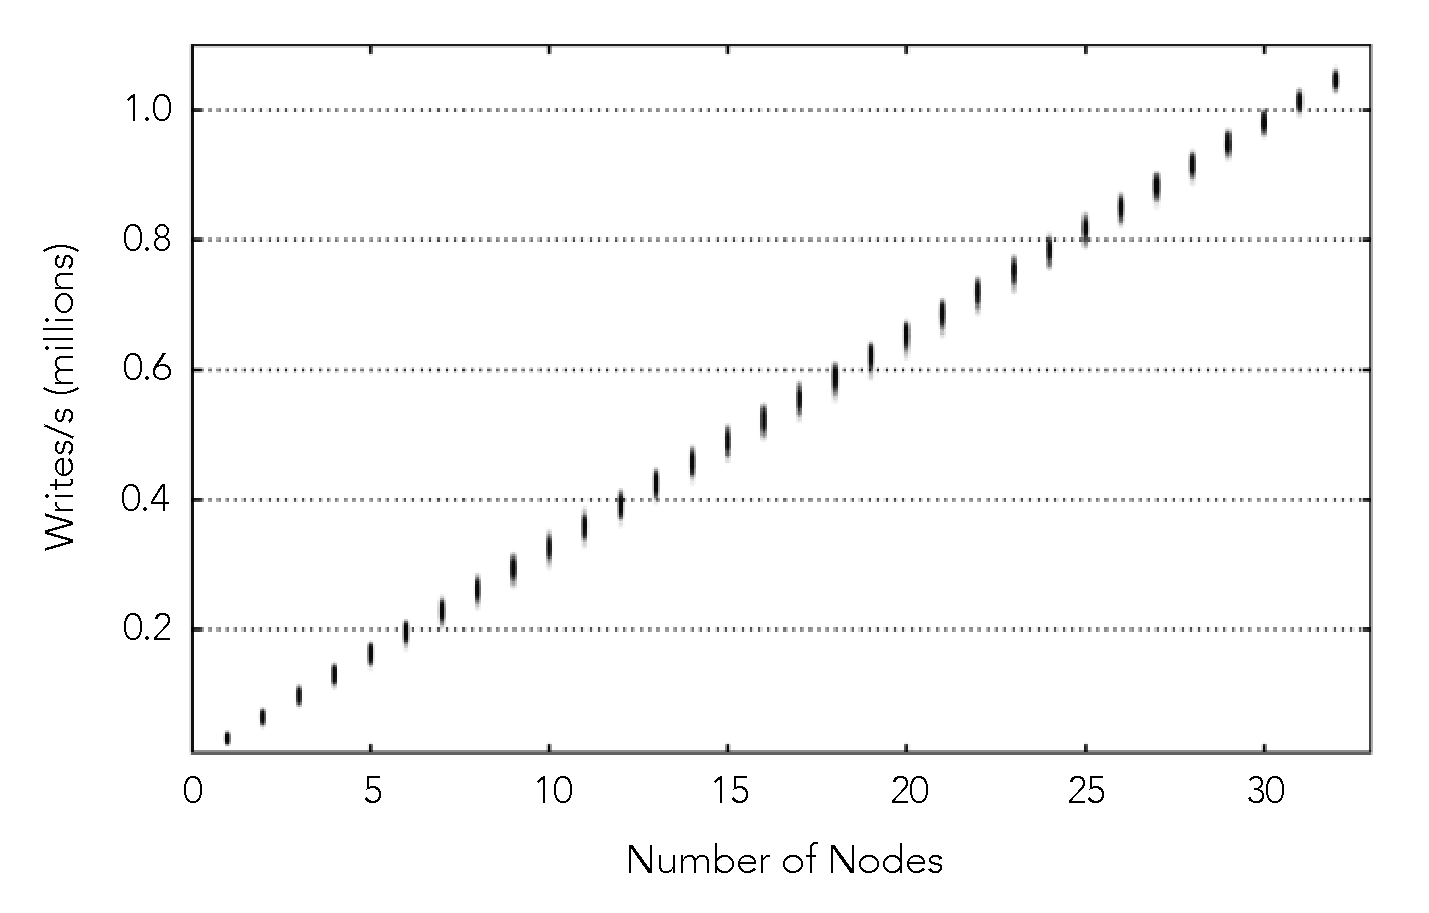
\includegraphics[width=0.7\textwidth]{figure_15.pdf}
  \caption{Write performance versus number of nodes. There is linear scaling in write performance with the number of nodes.}
  \label{fig:bigchain_writes_vs_nodes}
\end{figure}

Figure~\ref{fig:bigchain_writes_vs_nodes} shows data from the same experiment, except it shows how write throughput was affected by the number of nodes (rather than time).
The plot is both boring and exciting: it shows how write throughput increases linearly with the number of nodes.

\subsection{Other Experiments}
Appendix~\ref{appendix:benchmarks} contains descriptions and results of further experiments.
\section{BigchainDB Deployment}\label{sec:deployment}

\subsection{BigchainDB Use Cases}

Many BigchainDB use cases are like traditional blockchain use cases, except focused on situations where higher throughput, lower latency, or more storage capacity is necessary; where powerful querying or permissioning are helpful; or for simplicity of deployment since it feels like using a NoSQL database.
For example, BigchainDB can handle the throughput of high-volume payment processors, and directly store contracts receipts, or other related documents on the DB alongside the actual transaction.
Another example is “Bitcoin 2.0” applications, to keep transaction costs reasonable as the application scales\footnote{
As of February 2016, the fee required to ensure that a Bitcoin transaction goes through is about \$$0.10$~USD. There is no predefined fee for Bitcoin transactions; it's determined by market forces.
To estimate the fee, we can look at the fees that were paid in the last X blocks, and use that information to calculate a fee that will give a high probability that a transaction will go into the next block.
Usually a higher fee will give a higher priority to a transaction, but in the end, it's the miners that decide whether they want to include the transaction in the block or not.
Usually the fees are around $15$k-$20$k satoshi per $1000$ bytes, so that would be the average fee to pay.
Useful resources are blockchain.info \cite{blockchaininfo2015transaction_fees}, Tradeblock \cite{tradeblock} (in the charts, select fee/size), and the Bitcoin wiki page on transaction fees \cite{bitcoin2015fees}.
}.

Some BigchainDB use cases are also like traditional distributed DB use cases, except focused where blockchain characteristics can benefit: decentralization, immutability, and the ability to create and transfer digital assets. For example, improving DB reliability by not having a single point of failure, or storage of documents with secure time-stamping.

BigchainDB use cases include:
\begin{itemize}
 \item \textbf{Tracking intellectual property assets} along the licensing chain. BigchainDB can reduce licensing friction in channels connecting creators to audiences, and gives perfect provenance to digital artifacts. A typical music service has $38$ million songs—BigchainDB could store this information in a heartbeat, along with licensing information about each song and information about use by subscribers. In another example, consider a medium-sized photo marketplace running $100,000$ transactions a day; to put this on Bitcoin would cost \$$10,000$ per day and tie up the Bitcoin network.
 \item \textbf{Time stamping, receipts, and certification.} BigchainDB reduces legal friction by providing irrefutable evidence of an electronic action. And, BigchainDB is big enough that supporting information like receipts and certificates of authenticity (COAs) can be stored \textit{directly} on it, rather than linking to the document or storing a hash.
 \item \textbf{Legally-binding contracts} can be stored directly on the BigchainDB next to the transaction, in a format that is readable by humans and computers \cite{grigg2004ricardian}.
 \item \textbf{Creation and real-time movement of high-volume financial assets.} Only the owner of the asset can move the asset, rather than the network administrator like in previous database systems. This capability reduces costs, minimizes transaction latency, and enables new applications.
 \item \textbf{Tracking high-volume physical assets} along whole supply chain. BigchainDB can help reduce fraud, providing massive cost savings. Every RFID tag in existence could be entered on a BigchainDB.
 \item \textbf{Smart contracts} (decentralized processing), where the application must be fully decentralized and database functionality is crucial.
 \item \textbf{Data science} applications where the BigchainDB captures massive data streams, and data scientists can easily run queries against BigchainDB in their data mining and analytics tasks.
 \item \textbf{Improving database reliability} by creating resistance to single points of failure. This reliability helps move past the status quo where a single hack leads to massive data loss, like in Target, Sony, or the OPM \cite{ojeda2014target_hack}\cite{bluestone2014sony_hack}\cite{davis2015hacking}.
\end{itemize}

\subsection{Transaction Encryption}
Normally, transactions stored in BigchainDB aren't encrypted, but users can encrypt the payload if they want, using the encryption technology of their choice. (The payload of a transaction can be any valid JSON, up to some maximum size as explained below.) Other aspects of the transaction, such as the current owner's public key and the new owner's public key, aren't encrypted and can't be encrypted.

\subsection{BigchainDB Limitations}
Because BigchainDB is built on top of an existing ``big data'' database, it inherits many of the limitations of that database.

The first version of BigchainDB is built on top of RethinkDB, so it inherits some of RethinkDB's limitations, including a maximum of 32 shards per table (increasing to 64). While there's no hard limit on the document (transaction) size in RethinkDB, there is a recommended limit of 16MB for memory performance reasons. Large files can be stored elsewhere; one would store only the file location or hash (or both) in the transaction payload.

\subsection{BigchainDB Products \& Services}
We envision the following products and services surrounding BigchainDB:
\begin{enumerate}
 \item \textbf{BigchainDB: a blockchain database} with high throughput, high capacity, low latency, rich query support, and permissioning.
 \begin{itemize}
  \item For large enterprises and industry consortia creating new private trust networks, to take advantage of blockchain capabilities at scale or to augment their existing blockchain deployments with querying and other database functionality
  \item BigchainDB will be available in an out-of-the-box version that can be deployed just like any other DB, or customized versions (via services, or customized directly by the user).
  \item BigchainDB will include interfaces such as a REST API, language-specific bindings (e.g. for Python), RPC (like bitcoind), and command line. Below that will be an out-of-the-box core protocol, out-of-the-box asset overlay protocol \cite{dejonghe_spool}, and customizable overlay protocols.
  \item BigchainDB will support legally binding contracts, which are generated automatically and stored directly, in a format readable by both humans and computers \cite{grigg2004ricardian}. There will be out-of-box contracts for out-of-the-box protocols, and customizable contracts for customizable protocols.
  \item BigchainDB will offer cryptographic COAs, which can be generated automatically and stored directly on the BigchainDB. There will be out-of-box and customizable versions.
  \item BigchainDB is built on a large, open-source pre-existing database codebase that has been hardened on enterprise usage over many years. New code will be security-audited and open source.
 \end{itemize}
 \item \textbf{BigchainDB as a Service}, using a public BigchainDB instance, or a private BigchainDB with more flexible permissioning.
 \begin{itemize}
  \item For developers who want the benefits of blockchain databases without the hassle of setting up private networks.
  \item For cloud providers and blockchain platform providers who want scalable blockchain database as part of their service.
  \item For “Bitcoin 2.0” companies looking to keep transaction costs reasonable as they go to scale
  \item Main interfaces will be a REST API directly, REST API through cloud providers, and language-specific bindings (e.g. Python).
  \item With the features of the BigchainDB listed above.
 \end{itemize}
 \item \textbf{“Blockchain-ify your database”} service, to help others bring blockchain properties to other distributed DBs. Think MySqlChain, CassandraChain, and Neo4jChain.
 \begin{itemize}
  \item For DB vendors looking to extend their DB towards blockchain applications.
  \item For DB developers who want to play with blockchain technology.
 \end{itemize}
\end{enumerate}


\subsection{Timeline}
Like many, we have known about Bitcoin and blockchain scalability issues for years.
Here’s the timeline of how BigchainDB took shape:
\begin{itemize}
  \item Oct 2014 – Gave our first public talk on big data and blockchains \cite{mcconaghy2014blockchain}
  \item Apr 2015 – Preliminary investigations; paused the project to focus on our IP business
  \item Sep 2015 – Re-initiated the project; detailed design; building and optimizing
  \item Dec 2015 – Benchmark results of $100,000$ transactions/s
  \item Dec 2015 – Alpha version of the software integrated into an enterprise customer prototype
  \item Dec 2015 – Initial drafts of the whitepaper shared with some reviewers
  \item Jan 2016 – Benchmark results of $1,000,000$ transactions/s
  \item Feb 10, 2016 – BigchainDB was publicly announced
  \item Feb 10, 2016 – The first public draft of the whitepaper was released
  \item Feb 10, 2016 – Version 0.1.0 of the software was released open-source on GitHub\footnote{\url{http://github.com/bigchaindb/bigchaindb}. Core BigchainDB software is licensed under an Affero GNU Public License version 3 (AGPLv3). The BigchainDB drivers supported by ascribe GmbH are licensed under an Apache License (version 2.0).}. The software was not recommended for external use yet, but development was in the open.
  \item Apr 26, 2016 – Version 0.2.0 released
\end{itemize}

The current BigchainDB Roadmap can be found in the \texttt{bigchaindb/org} repository on GitHub\footnote{\url{https://github.com/bigchaindb/org/blob/master/ROADMAP.md}}.
\section{Conclusion}\label{sec:conclusion}

This paper has introduced BigchainDB. BigchainDB fills a gap in the decentralization ecosystem: a decentralized database, at scale.
BigchainDB performance points to $1$ million writes per second, sub-second latency, and petabyte capacity.
It has easy-to-use and efficient querying.
It features a rich permissioning system that supports public and private blockchains.
It is complementary to decentralized processing technologies (smart contracts) and decentralized file systems, and can be a building block within blockchain platforms.

\section{Acknowledgments}\label{sec:acknowledgments}

We would like to thank the following people for their reviews, suggested edits and helpful advice: 
David Holtzman, 
Jim Rutt, 
Evan Schwartz, 
Ian Grigg, 
Benjamin Bollen, 
Carsten Stocker, 
Adi Ben-Ari, 
Jae Kwon, 
Juan Benet 
and Bruce Pon. 
A big spark to this project came from conversations with Jim Rutt going back to early ascribe days, about the need for scale and how to reconcile it with latency and voting. We are grateful for all advice we have received, from all the amazing folks involved.
If you have feedback, please email \href{mailto:trent@bigchaindb.com}{trent@bigchaindb.com}.

\begin{appendices}
\section{Glossary}\label{appendix:glossary}

\noindent\textbf{SQL DB} – a database that stores data in table format and supports the Structured Query Language (SQL); a relational database. Example: MySQL.

\medskip
\noindent\textbf{Ledger} – a database that stores data in a table format, where entries are economic transactions

\medskip
\noindent\textbf{NoSQL DB} – a database that stores data in a non-table format, such as key-value store or graph store. Example: RethinkDB.

\medskip
\noindent\textbf{NoQL DB} – a database without any query language to speak of. Obviously, this hinders data management. Example: Bitcoin blockchain.

\medskip
\noindent\textbf{Distributed DB} – a database that distributes data among more than one node in a network\footnote{Sometimes there is confusion, and “distributed” is used when the actual meaning is that of “decentralized”, most notably with the term “distributed ledger”.}. Example: RethinkDB.

\medskip
\noindent\textbf{Fully replicated DB} – a distributed DB where every node holds all the data.

\medskip
\noindent\textbf{Partially replicated DB} – a distributed DB where every node holds a fraction of the data.

\medskip
\noindent\textbf{Decentralized DB} – a DB where no single node owns or controls the network.

\medskip
\noindent\textbf{Immutable DB} – a DB where storage on the network is tamper-resistant.

\medskip
\noindent\textbf{Blockchain DB} – a distributed, decentralized, immutable DB, that also has ability for creation \& transfer of assets without reliance on a central entity.

\medskip
\noindent\textbf{Bitcoin blockchain} – a specific NoQL, fully-replicated, blockchain DB.

\medskip
\noindent\textbf{BigchainDB} – a specific NoSQL\footnote{There can be SQL support to via wrapping the NoSQL functionality or using the BigchainDB design on a distributed SQL DB}, partially-replicated, blockchain DB.
\section{Blockchain Scalability Proposals}\label{appendix:blockchain_scalability}

Here, we review some proposals to solve the Strong Byzantine Generals’ (SBG) problem while scaling the blockchain, and to allow blockchain-like behavior at greater scales.
This list is not intended to be exhaustive.

\subsection{Base Consensus Approaches}

Consensus refers to the way nodes on a blockchain network approve or reject new transactions.
These approaches differ in (a) how a node becomes a voting node, and (b) how each node’s voting weight is set.
These choices can impact the blockchain’s performance.

\medskip
\noindent\textbf{Proof of Work (POW).} POW is the baseline approach used by the Bitcoin blockchain.
There is no restriction on who can enter the network as a voter. 
A node is chosen at random, proportional to the processing ability it brings to the network, according to a mathematical puzzle — its “hash rate”. 
Work \cite{back2002hashcash} may be SHA256 hashing (the algorithm used by Bitcoin), scrypt hashing (used by Litecoin), or something else.

POW has a natural tendency towards centralization. It is a contest to garner the most hashing power. Power is currently held by a handful of mining pools.

\medskip
\noindent\textbf{Proof of Stake (POS)} \cite{bitcoin2015pos}. In the POS model, there is no restriction on who can enter the network. 
To validate a block, a node is chosen at random, proportionally to how much “stake” it has. 
“Stake” is a function of the amount of coin held, and sometimes of “coin age, a measurement of how many days have passed since last time the coin voted.

POS promises lower latency and does not have the extreme computational requirements of POW.

However, over the last couple years, POS proposals have evolved as issues are identified (e.g. “nothing at stake,” “rich get richer,” and “long range attacks”) and fixes proposed. 
These fixes have resulted in POS protocols becoming increasing complex. 
Complex systems generally have more vulnerabilities, compromising security.

\medskip
\noindent\textbf{Federation.} A federated blockchain is composed of a number of nodes operating under rules set for or by the group. 
Each member of a federation typically has an equal vote, and each federation has its own rules about who can join as voting node. 
Typically, the majority or 2/3 of the voting nodes need to agree, for a transaction or block to be accepted (“quorum”).

Federations may have of any number of voting nodes.
More nodes mean higher latency, and less nodes means the federation is not as decentralized as many would like.
Besides voting nodes, other nodes may have permission to issue assets, transfer assets, read, and so on (super-peer P2P network).

Membership rules for voting nodes can vary widely between models.
In the (pre-acquisition) Hyperledger model, the requirement was having a TLD and SSL certificate \cite{bitsmith2014hyperledger}. 
In the original Stellar model, membership was based on a social network, until it was forked \cite{kim2014safety}. 
In Tendermint \cite{kwon2014tendermint}, Slasher \cite{buterin2014slasher, buterin2014slasher_ghost}, and Casper \cite{zamfir2015casper}, anyone could join by posting a fixed bond as a security deposit, which would be lost if the voting node were to act maliciously\footnote{These are arguably proof of stake. It depends whether one’s definition of “proof of stake” means “has a stake, anywhere” versus “degree of voting power is a function of amount at stake”.}.

Membership rules can directly affect the size of the federation.
For example, in Tendermint, the lower the security deposit (bond), the more voting nodes there are likely to be.

Federations imply that to be a voting node, one must reveal their identity.
This means they are not as suitable where censorship resistance is a key design spec.
This is different than POW and POS.

\subsection{Consensus Mashups}
The base consensus approaches described above can be creatively combined.

\medskip
\noindent\textbf{Hierarchy of POW—Centralized.} Big Bitcoin exchanges operate their own internal DBs of transactions, then synchronize a summary of transactions with the Bitcoin blockchain periodically. 
This is similar to how stock exchange “dark pools” operate—financial institutions make trades outside the public stock exchange, and periodically synchronize with the public exchange.

\medskip
\noindent\textbf{Hierarchy of Small Federation—Big Federation.} An example is AI Coin \cite{aicoin}. 
The top level has 5 power nodes with greater influence, and the bottom level has 50 nodes with less influence.

\medskip
\noindent\textbf{Hierarchy of POW—Federation.} An example is Factom \cite{factom}. 
The bottom level is a document store; then document hashes are grouped together in higher and higher levels, Merkle tree style; and the top level the Merkle tree root is stored on the Bitcoin blockchain.

\medskip
\noindent\textbf{POW then POS.} An example is the Ethereum rollout plan. 
The Ethereum team realized that if only a few coins were in circulation in a POS model, it would be easy for a bad actor to dominate by buying all the coins, and that they needed more time to develop an efficient yet trustworthy POS algorithm. 
Therefore, Ethereum started with POW mining to build the network and get coins into wider circulation, and plans to switch once there are sufficient coins and the POS approach is ready.

\medskip
\noindent\textbf{X then Centralized then X’.} This model is applied when the consensus algorithm being used gets broken. 
Voting is temporarily handled by the project’s managing entity until a fixed version of the algorithm is developed and released. 
This happened with Stellar. Stellar started as a federation but the project was split in a fork \cite{kim2014safety}. 
Stellar ran on a single server in early 2015 while a new consensus protocol \cite{mazieres2015stellar} was developed and released in April 2015 \cite{kim2014stellar}. 
The new version is like a federation, but each node chooses which other nodes to trust for validation \cite{mazieres2015stellar}. 
Another example of this model is Peercoin, one of the first POS variants. After a fork in early 2015, the developer had to sign transactions until a fix was released \cite{peercoin}.

\subsection{Engineering Optimizations}
This section reviews some of the possible steps to improve the efficiency and throughput of existing blockchain models.

\medskip
\noindent\textbf{Shrink Problem Scope.} This range of optimizations aims to make the blockchain itself smaller. 
One trick to minimize the size of a blockchain is to record only unspent outputs. 
This works if the history of transactions is not important, but in many blockchain applications, from art provenance to supply chain tracking, history is crucial. 
Another trick, called Simple Payment Verification (SPV), is to store only block headers rather than the full block. 
It allows a node to check if a given transaction is in the block without actually holding the transactions. 
Mobile devices typically use Bitcoin SPV wallets. Cryptonite is an example that combines several of these tricks \cite{cryptonite}. 
These optimizations makes it easier for nodes to participate in the network, but ultimately does not solve the core consensus problem.

\medskip
\noindent\textbf{Different POW hashing algorithm.} This kind of optimization seeks to make the hashing work performed by the network more efficient. 
Litecoin is one of several models using scrypt hashing instead of Bitcoin’s SHA256 hashing, requiring about 2/3 less computational effort than SHA256. 
This efficiency gain does not improve scalability, because it still creates a hash power arms race between miners.

\medskip
\noindent\textbf{Compression.} Data on a blockchain has a particular structure, so it is not out of the question that the right compression algorithm could reduce size by one or more orders of magnitude. 
This is a nice trick without much compromise for a simple transaction ledger. 
Compression typically hinders the ability to efficiently query a database.

\medskip
\noindent\textbf{Better BFT Algorithm.} The first solution to the Byzantine Generals problem was published in 1980 \cite{pease1980reaching}, and since that time many proposals have been published at distributed computing conferences and other venues. 
Modern examples include Aardvark \cite{clement2009making} and Redundant Byzantine Fault Tolerance (RBFT) \cite{aublin2013rbft}. 
These proposals are certainly useful, but in on their own do not address the need for Sybil tolerance (attack of the clones problem).

\medskip
\noindent\textbf{Multiple Independent Chains.} Here, the idea is to have multiple blockchains, with each chain focusing on a particular set of users or use cases and implementing a model best suited to those use cases. 
The countless centralized DBs in active use operate on this principle right now; each has a specific use case. 
We should actually expect this to happen similarly with blockchains, especially privately deployed ones but also for public ones. 
It is the blockchain version of the Internet’s Rule 34: “If it exists there is blockchain of it.”

For public examples, you could use Ethereum if you want decentralized processing, Primecoin if you want POW to be slightly more helpful to the world, and Dogecoin if you want much cute, very meme. 
For private examples, organizations and consortiums will simply deploy blockchains according to their specific needs, just as they currently deploy DBs and other compute infrastructure.

A challenge lies in security: if the computational power in a POW blockchain or coin value in a POS blockchain is too low, they can be overwhelmed by malicious actors. 
However, in a federation model, this could be workable, assuming that an individual blockchain can meet the specific use case’s performance goals, in particular throughput and latency.

\medskip
\noindent\textbf{Multiple Independent Chains with Shared Resources for Security.} Pegged sidechains are the most famous example, where mining among chains has the effect of being merged \cite{back2002hashcash}. 
SuperNET \cite{galt2014supernet} and Ethereum’s hypercubes and multichain proposals \cite{buterin2014hypercubes} fit in this category. 
However, if the goal is simply to get a DB to run at scale, breaking the DB into many heterogeneous sub-chains adds cognitive and engineering complexity and introduces risk.

\medskip
\noindent\textbf{$\dots$and more}. The models described above are just a sampling. 
There continue to be innovations (and controversy \cite{bitcoin-blocksize, popper2016bitcoin_crisis}). 
For example, a proposed change to the Bitcoin blockchain called Bitcoin-NG \cite{eyal2015bitcoin} aims to reduce the time to first confirmation while minimizing all other changes to the Bitcoin blockchain design. 
The Bitcoin roadmap \cite{bitcoin2015capacity, maxwell2015capacity} contains many other ideas, most notably segregated witness \cite{wuille_segregated_witness}.
\section{Case Study: DNS as a Decentralized Internet-scale Database}\label{sec:dns}

\subsection{Introduction}
In the previous section, we reviewed big data” distributed databases (DBs), highlighting their Internet-level scalability properties and solid foundation in consensus via Paxos.
We also highlighted the core weakness: centralized control where a trusted third party is always holding the keys.

We are left with the question: Are there any precedents for distributed DBs going not only to Internet scale, but in a decentralized and trusted fashion?

There is one DB that not only operates at Internet scale, but also has decentralized control, and is crucial to the functioning of the Internet as we know it: the Domain Name System (DNS).

\subsection{History of DNS}

By the early $1980$s, the rapid growth of the Internet made managing numeric domains a major bookkeeping headache \cite{dnshistory}.
To address this, in $1983$ Jon Postel proposed the DNS.
The DNS was originally implemented as a centralized DB, operated by the U.S. government.
In $1993$ the U.S. government handed control to Network Solutions Inc. (NSI), a private corporation.

NSI faced a dual challenge. It had to make the DNS function effectively, but in a way that took power away from any single major stakeholder, including the U.S. government and even NSI itself.
David Holtzman, Chief Technology Officer of NSI, architected a solution: a federation of nodes spread around the globe, where each node’s interests were as orthogonal as possible to the interests of all the other nodes, in order to prevent collusion \cite{dnshistory}.
Holtzman deployed this DB while NSI’s Chief Executive Officer, Jim Rutt, worked vigorously to hold off the objections of the U.S. Commerce Department and U.S. Department of Defence, which had hoped to maintain control \cite{schwartz2001badboy}.
In the late 90s, NSI handed off DNS oversight to the Internet Corporation for Assigned Names and Numbers (ICANN), a new non-governmental, non-national organization \cite{dnshistory}.

At its core, DNS is simply a mapping from a domain name (e.g. amazon.com) to a number (e.g. $54.93.255.255$).
People trust the DNS because no one really controls it; it’s administered by ICANN.

The DNS was architected to evolve and extend over time.
For example, the original design did not include sufficient security measures, so the DNS Security Extensions (DNSSEC) were added to bring security while maintaining backwards compatibility \cite{icann2014dnssec}.

It is hard to imagine something more Internet scale than the database underpinning the Internet’s domain name system.
The decentralized DNS successfully deployed at Internet scale, both in terms of technology and governance.
ICANN has not always been popular, but it has lasted and held the Internet together through its explosive growth, and survived heavy pressure from governments, corporations, and hackers.

Domain names have digital scarcity via a public ledger that requires little extra trust by the user.
There can be only one amazon.com in the DNS model. But DNS is a consensual arrangement.
Anyone could create an alternative registry that could work in a similar manner, assigning amazon.com to someone else.
The alternative registry would be near useless, however, because there is a critical mass of users that have already voted on which domain system will be in use, with their network devices by choosing what name server to use, and with their wallets by purchasing and using domain names within the existing DNS system.

\subsection{Strengths and Weaknesses}
\medskip
\noindent\textbf{Weaknesses.} The DNS does not address the challenge of large scale data storage, or for the blockchain characteristics of immutability or creation \& transfer of assets.
But, it didn’t aim to.

\medskip
\noindent\textbf{Strengths.} The DNS shows that decentralized control, in the form of federations, can work at Internet scale.
It also demonstrates that it is crucial to get the right federation, with the right rules.

\section{Other Experiments}\label{appendix:benchmarks}

\subsection{Experimental Setup}\label{subsec:benchmarks_setup}

To test the writing performance, we have a process that inserts a block in the database in an infinite loop.

The block is a valid block with small transactions.
In our case, we used transactions without any payload. 
An entire block occupies about $900$KB.

\begin{minipage}{\linewidth}
  \begin{lstlisting}[style=python]
  while True:
    r.table(table).insert(r.json(BLOCK_SERIALIZED), durability='soft').run(conn)\end{lstlisting}
\end{minipage}

In $\mathtt{hard}$ durability mode, writes are committed to disk before acknowledgments are sent; in $\mathtt{soft}$ mode, writes are acknowledged immediately after being stored in memory.

This means that the insert will block until RethinkDB acknowledges that the data was cached.
In each server we can start multiple processes.

\medskip
\noindent\textbf{Write Units.} Let’s define \textit{$1$ write unit} as being 1 process.
For example, in a $32$ node cluster, with each node running $2$ processes, we would have $64$ write units.
This will make it easier to compare different tests.

\medskip
\noindent\textbf{Sharding} in distributed datastores means partitioning a table so that the data can be evenly distributed between all nodes in the cluster.
In most distributed datastores, there is a maximum number of shards per table. For RethinkDB, that limit is $32$ shards per table.

In RethinkDB, a shard is also called a primary replica, since by default the replication factor is $1$.
Increasing the replication factor produces secondary replicas that are used for data redundancy. If a node holding a primary replica goes down, another node holding a secondary replica of the same data can step up and become the primary replica.

\medskip
\noindent\textbf{Compute Resources.} For these tests we are using $32$-core AWS EC2 instances with SSD storage and 10Gbps network connections ($\mathtt{c3.8xlarge}$).
For the tests, we used either $32$- or $64$-node clusters all running in the same AWS region.

\subsection{Experiments on Throughput}
The experimental setup is like the setup described in section \ref{subsec:benchmarks_setup}. 

\subsubsection{Experiment 1}\label{subsubsec:appendix_benchmarks_exp1}

\medskip
\noindent\textbf{Settings:}
\begin{itemize}
 \item \textbf{Number of nodes:} $32$
 \item \textbf{Number of processes:} $2$ processes per node
 \item \textbf{Write units:} $32 \times 2 = 64$ write units
\end{itemize}

\medskip
\noindent\textbf{Results:}
\begin{itemize}
 \item \textbf{Output:} stable $1$K writes per second
\end{itemize}

This was the most successful experiment. We were able to reach a stable output of $1$K blocks per second. The load on the machines is stable and the IO is at an average of $50-60 \%$.

Other tests have shown that increasing the number write units per machine can lead to a stable performance up to $1.5$K writes per second but the load on the nodes would increase until the node would eventually fail. 
This means that we are able to handle bursts for a short amount of time ($10-20$ min).

This test can be used has a baseline for the future in where $64$ writes equal $1$K transactions per second. 
Or, that each write unit produces an output of $(1000/64) \approx 64$ writes per second.

\subsubsection{Experiment 2}\label{subsubsec:appendix_benchmarks_exp2}
\medskip
\noindent\textbf{Settings:}
\begin{itemize}
 \item \textbf{Number of nodes:} $32$
 \item \textbf{Number of processes:}
 \begin{itemize}
  \item$16$ nodes running $2$ processes
  \item$16$ nodes running $3$ processes
 \end{itemize}
 \item \textbf{Write units:} $16 \times 3 + 16 \times 2 = 80$ write units
 \item \textbf{Expected output:} $1.25$K writes per second
\end{itemize}

\medskip
\noindent\textbf{Results:}
\begin{itemize}
 \item \textbf{Output:} stable $1.2$K writes per second
\end{itemize}

Increasing a bit the number of write units shows an increase in output close to the expected value but in this case the IO around $90\%$ close to the limit that the machine can handle.

\subsubsection{Experiment 3}\label{subsubsec:appendix_benchmarks_exp3}
\medskip
\noindent\textbf{Settings:}
\begin{itemize}
 \item \textbf{Number of nodes:} $32$
 \item \textbf{Number of processes:}
 \begin{itemize}
  \item$16$ nodes running $2$ processes
  \item$16$ nodes running $4$ processes
 \end{itemize}
 \item \textbf{Write units:} $16 \times 4 + 16 \times 2 = 96$ write units
 \item \textbf{Expected output:} $1.5$K writes per second
\end{itemize}

\medskip
\noindent\textbf{Results:}
\begin{itemize}
 \item \textbf{Output:} stable $1.4$K writes per second
\end{itemize}

This test produces results similar to previous one. 
The reason why we don't quite reach the expected output may be because RethinkDB needs time to cache results and at some point increasing the number of write units will not result in an higher output. 
Another problem is that as the RethinkDB cache fills (because the RethinkDB is not able to flush the data to disk fast enough due to IO limitations) the performance will decrease because the processes will take more time inserting blocks. 

\subsubsection{Experiment 4}\label{subsubsec:appendix_benchmarks_exp4}
\medskip
\noindent\textbf{Settings:}
\begin{itemize}
 \item \textbf{Number of nodes:} $64$
 \item \textbf{Number of processes:} $1$ process per node
 \item \textbf{Write units:} $64 \times 1 = 64$ write units
 \item \textbf{Expected output:} $1$K writes per second
\end{itemize}

\medskip
\noindent\textbf{Results:}
\begin{itemize}
 \item \textbf{Output:} stable $1$K writes per second
\end{itemize}

In this case, we are increasing the number of nodes in the cluster by $2\times$. 
This won't have an impact in the write performance because the maximum amount of shards per table in RethinkDB is $32$ (RethinkDB will probably increase this limit in the future).
What this provides is more CPU power (and storage for replicas, more about replication in the next section). 
We just halved the amount write units per node maintaining the same output. 
The IO in the nodes holding the primary replica is the same has Experiment \ref{subsubsec:appendix_benchmarks_exp1}. 

\subsubsection{Experiment 5}\label{subsubsec:appendix_benchmarks_exp5}
\medskip
\noindent\textbf{Settings:}
\begin{itemize}
 \item \textbf{Number of nodes:} $64$
 \item \textbf{Number of processes:} $2$ process per node
 \item \textbf{Write units:} $64 \times 2 = 128$ write units
 \item \textbf{Expected output:} $2000$ writes per second
\end{itemize}

\medskip
\noindent\textbf{Results:}
\begin{itemize}
 \item \textbf{Output:} unstable $2$K (peak) writes per second
\end{itemize}

In this case, we are doubling the amount of write units. 
We are able to reach the expected output, but the output performance is unstable due to the fact that we reached the IO limit on the machines. 

\subsubsection{Experiment 6}\label{subsubsec:appendix_benchmarks_exp6}
\medskip
\noindent\textbf{Settings:}
\begin{itemize}
 \item \textbf{Number of nodes:} $64$
 \item \textbf{Number of processes:}
 \begin{itemize}
  \item$32$ nodes running $1$ processes
  \item$32$ nodes running $2$ processes
 \end{itemize}
 \item \textbf{Write units:} $32 \times 2 + 32 \times 1 = 96$ write units
 \item \textbf{Expected output:} $1.5$K writes per second
\end{itemize}

\medskip
\noindent\textbf{Results:}
\begin{itemize}
 \item \textbf{Output:} stable $1.5$K writes per second
\end{itemize}

This test is similar to Experiment \ref{subsubsec:appendix_benchmarks_exp3}. 
The only difference is that now the write units are distributed between $64$ nodes meaning that each node is writing to its local cache and we don't overload the cache of the nodes like we did with Experiment \ref{subsubsec:appendix_benchmarks_exp3}. 
This is another advantage of adding more nodes beyond $32$.

\subsection{Experiments on Replication}

Replication is used for data redundancy.
In RethinkDB we are able to specify the number of shards and replicas per table.
Data in secondary replicas is no directly used, it’s just a mirror of a primary replica and used in case the node holding the primary replica fails.

RethinkDB does a good job trying to distribute data evenly between nodes.
We ran some tests to check this.

By increasing the number of replicas we also increase the number of writes in the cluster.
For a replication factor of $2$ we double the amount of writes on the cluster, with a replication factor of $3$ we triple the amount of writes and so on.

With $64$ nodes and since we can only have $32$ shards we have $32$ nodes holding shards (primary replicas)

With a replication factor of $2$, we will have $64$ replicas ($32$ primary replicas and $32$ secondary replicas).
Since we already have $32$ nodes holding the $32$ shards/primary replicas RethinkDB uses the other $32$ nodes to hold the secondary replicas. 
So in a $64$ node cluster with $32$ shards and a replication factor of $2$, $32$ nodes will be holding the primary replicas and the other $32$ nodes will be holding the secondary replicas.

If we run Experiment \ref{subsubsec:appendix_benchmarks_exp4} again with this setup, except now with a replication factor of $2$, we get twice the amount of writes. 
A nice result is that the IO in the nodes holding the primary replicas does not increase when compared to Experiment \ref{subsubsec:appendix_benchmarks_exp4} because all of the excess writing is now being done the $32$ nodes holding the secondary replicas.

Also regarding replication: if I have a $64$ node cluster and create a table with $32$ shards, $32$ nodes will be holding primary replicas and the other nodes do not hold any data. 
If I create another table with $32$ shards RethinkDB will create the shards in the nodes that where not holding any data, evenly distributing the data.

\end{appendices}

{\footnotesize\bibliography{bigchain.bib}{}}
\bibliographystyle{unsrt}

\end{document}
